% 本文件定位：SM 分卷（概念与框架、社会认知、轻度与进阶实践、绳缚与重度技法、健康安全；已并入《SM 入门指南》译本内容，全书共五章）

\documentclass[12pt,UTF8]{ctexbook}

% 设置纸张信息
\usepackage[a4paper]{geometry}
\geometry{
    inner=2cm,
    outer=2cm,
    top=2.5cm,
    bottom=2.5cm
}

% 设置字体
\usepackage{xeCJK}
\setCJKmainfont{SimSun}[BoldFont=SimHei, ItalicFont=KaiTi]
\setCJKsansfont{SimHei}
\setCJKmonofont{SimSun}

% ===== 符号字体回退（r75）：带圈数字 / 罗马数字 / 希腊字母 / 数学符号 / 制表符 ----
%   背景：西文主字体 Latin Modern 与中文字体 SimSun 均不覆盖下列字符，
%   不回退则 xelatex 报 Missing character，PDF 对应位置留白（等于丢知识点）。
%   自检：编译后统计 <file>.log 中 Missing character 条数，应为 0。
\usepackage{newunicodechar}
\newfontfamily\symbolfallback{SimSun}           % 带圈数字/罗马数字/希腊字母/数学符号/制表符/几何图形
\newfontfamily\symbolfallbackx{Segoe UI Symbol} % 警告三角等符号
\newunicodechar{①}{{\symbolfallback\char"2460}}
\newunicodechar{②}{{\symbolfallback\char"2461}}
\newunicodechar{③}{{\symbolfallback\char"2462}}
\newunicodechar{④}{{\symbolfallback\char"2463}}
\newunicodechar{⑤}{{\symbolfallback\char"2464}}
\newunicodechar{⑥}{{\symbolfallback\char"2465}}
\newunicodechar{⑦}{{\symbolfallback\char"2466}}
\newunicodechar{⑧}{{\symbolfallback\char"2467}}
\newunicodechar{⑨}{{\symbolfallback\char"2468}}
\newunicodechar{⑩}{{\symbolfallback\char"2469}}
\newunicodechar{Ⅰ}{{\symbolfallback\char"2160}}
\newunicodechar{Ⅱ}{{\symbolfallback\char"2161}}
\newunicodechar{Ⅲ}{{\symbolfallback\char"2162}}
\newunicodechar{Ⅳ}{{\symbolfallback\char"2163}}
\newunicodechar{Ⅴ}{{\symbolfallback\char"2164}}
\newunicodechar{Ⅵ}{{\symbolfallback\char"2165}}
\newunicodechar{Ⅶ}{{\symbolfallback\char"2166}}
\newunicodechar{Ⅷ}{{\symbolfallback\char"2167}}
\newunicodechar{Ⅸ}{{\symbolfallback\char"2168}}
\newunicodechar{Ⅹ}{{\symbolfallback\char"2169}}
\newunicodechar{Ⅺ}{{\symbolfallback\char"216A}}
\newunicodechar{Ⅻ}{{\symbolfallback\char"216B}}
\newunicodechar{α}{{\symbolfallback\char"03B1}}
\newunicodechar{β}{{\symbolfallback\char"03B2}}
\newunicodechar{γ}{{\symbolfallback\char"03B3}}
\newunicodechar{δ}{{\symbolfallback\char"03B4}}
\newunicodechar{ε}{{\symbolfallback\char"03B5}}
\newunicodechar{ζ}{{\symbolfallback\char"03B6}}
\newunicodechar{η}{{\symbolfallback\char"03B7}}
\newunicodechar{θ}{{\symbolfallback\char"03B8}}
\newunicodechar{ι}{{\symbolfallback\char"03B9}}
\newunicodechar{κ}{{\symbolfallback\char"03BA}}
\newunicodechar{λ}{{\symbolfallback\char"03BB}}
\newunicodechar{μ}{{\symbolfallback\char"03BC}}
\newunicodechar{ν}{{\symbolfallback\char"03BD}}
\newunicodechar{ξ}{{\symbolfallback\char"03BE}}
\newunicodechar{ο}{{\symbolfallback\char"03BF}}
\newunicodechar{π}{{\symbolfallback\char"03C0}}
\newunicodechar{ρ}{{\symbolfallback\char"03C1}}
\newunicodechar{ς}{{\symbolfallback\char"03C2}}
\newunicodechar{σ}{{\symbolfallback\char"03C3}}
\newunicodechar{τ}{{\symbolfallback\char"03C4}}
\newunicodechar{υ}{{\symbolfallback\char"03C5}}
\newunicodechar{φ}{{\symbolfallback\char"03C6}}
\newunicodechar{χ}{{\symbolfallback\char"03C7}}
\newunicodechar{ψ}{{\symbolfallback\char"03C8}}
\newunicodechar{ω}{{\symbolfallback\char"03C9}}
\newunicodechar{≠}{{\symbolfallback\char"2260}}
\newunicodechar{≈}{{\symbolfallback\char"2248}}
\newunicodechar{≤}{{\symbolfallback\char"2264}}
\newunicodechar{≥}{{\symbolfallback\char"2265}}
\newunicodechar{─}{{\symbolfallback\char"2500}}
\newunicodechar{■}{{\symbolfallback\char"25A0}}
\newunicodechar{⚠}{{\symbolfallbackx\char"26A0}}

% 图片相关设置
\usepackage{graphicx}
\usepackage{float}
\graphicspath{{Images/}}

% 颜色支持
\usepackage{color}

% 绘制流程图
\usepackage{tikz}
\usetikzlibrary{shapes,arrows,positioning,calc}

% 表格相关设置
\usepackage{tabularx}
\usepackage{booktabs}

% 彩色盒子环境
\usepackage{tcolorbox}

% BibTeX参考文献支持
\usepackage{natbib}
\bibliographystyle{plainnat}

% 超链接与 PDF 书签（hidelinks：不在正文显示彩色边框）
\usepackage[hidelinks]{hyperref}

% 页眉页脚
\usepackage{fancyhdr}
\pagestyle{fancy}
\lhead{}
\chead{}
\rhead{\bfseries \leftmark}
\lfoot{}
\cfoot{\thepage}
\rfoot{}
\renewcommand{\headrulewidth}{0.4pt}
\renewcommand{\footrulewidth}{0pt}

% 段落间距
\setlength{\parskip}{0.5em}
\setlength{\parindent}{2em}

% 目录格式设置
\usepackage{titletoc}
\usepackage{enumitem}% 支持 \begin{itemize}[leftmargin=2cm] 等带可选参数的列表（与 male.tex 一致）
\titlecontents{chapter}[0pt]{\vspace{3mm}\bfseries}{\thecontentslabel\hspace{1em}}{}{\titlerule*[8pt]{.}\contentspage}[\vspace{2mm}]
\titlecontents{section}[3em]{\contentslabel[\thecontentslabel]{2em}\hspace{1em}}{}{}{\titlerule*[6pt]{.}\contentspage}
\titlecontents{subsection}[5em]{\contentslabel[\thecontentslabel]{3em}\hspace{1em}}{}{}{\titlerule*[4pt]{.}\contentspage}

% 标题格式
\ctexset{
    part/name={第,篇},
    part/number={\chinese{part}},
    chapter/name={第,章},
    chapter/number={\chinese{chapter}}
}

% 章节摘要环境
\newenvironment{chapterabstract}[1][摘要]{
    \vspace{0.5em}
    \begin{center}\bfseries{#1}\end{center}
    \vspace{0.5em}
    \begin{quote}
    }{
    \end{quote}
    \vspace{0.5em}
}

% 重点标记
\newcommand{\important}[1]{{\color{red} \bfseries #1}}

% 关键词强调
\newcommand{\keyword}[1]{\textbf{#1}}

\title{\heiti\zihao{0} 性学大全指南·SM 分卷}
\author{}
\date{}

\begin{document}

\maketitle

\frontmatter

\chapter{前言}

本书是《性学大全指南》的\keyword{SM 分卷}，独立于共通卷（0\_book.tex）、男性卷（1\_male.tex）、女性卷（2\_female.tex）与性爱实践卷（3\_position.tex）单独成册，内容聚焦于成年人之间\keyword{知情同意}的 SM/BDSM 实践——概念与社会认知、安全框架、角色与心理、轻度实践、进阶技术与健康安全，并吸收了三叶《我的身体，我的心》中文译本中的实践内容（已按科学框架改写、整理与安全校订）。

全书共五章：第一章　SM 概述：概念、框架与社会认知；第二章　角色、动机与亲密关系；第三章　伴侣间引入 SM：沟通、风险与边界；第四章　轻度 SM：入门实践；第五章　进阶实践与健康安全（含绳缚、重度玩法与安全细则）。

\begin{tcolorbox}[colback=pink!5!white,colframe=red!50!black,title=使用说明]
本卷讨论的是成年人之间自愿、私密、知情同意的 SM/BDSM。首要原则贯穿全书：安全（Safe）、理智（Sane）、知情同意（Consensual）——任何涉及未成年人、非自愿对象或造成不可逆伤害的行为均不属于本卷讨论范畴，而为法律与伦理所禁止。译本实践内容带有特定文化背景（原文以日本语境写成），阅读与实践时请始终以各章的安全原则为准。
\end{tcolorbox}

\tableofcontents

\mainmatter

\chapter{SM 概述：概念、框架与社会认知}

本章回答“SM 是什么”：从大众误解与现代性学定位讲起，给出 SSC/RACK 安全框架与安全词、事后照护两个基础机制，再梳理 SM 的历史脉络、术语体系与社会态度，为后续各章的实践内容建立统一的认知与安全基线。

SM 是 Sadism（施虐）与 Masochism（受虐）的合称，广义上指在\textbf{知情同意}的前提下，通过权力交换、感官刺激（捆绑、击打、感官剥夺等）获得性唤起与愉悦的亲密实践。

\begin{itemize}
\item \textbf{核心三原则（SSC）}：安全（Safe——不造成不可逆伤害）、理智（Sane——清醒状态下协商）、同意（Consensual——所有环节可随时撤回）
\item \textbf{它不是什么}：不是暴力（暴力无同意，SM 的同意是前提与核心）；不是心理疾病（ICD-11 已将自愿 SM 移出精神障碍）；不是"一人永远凌驾另一人"——场景中的权力是\textbf{协议授予、随时收回}的
\item \textbf{本卷内容}：工具与技巧、安全与急救（绳缚安全、灌肠边界、电击玩具）、心理机制（痛觉转化、情绪跌落 drop）与事后护理——参见各专节
\item \textbf{入门路径}：先学沟通与安全词，再学工具；先轻后重，先看后做；阅读靠谱科普，远离"猛料"教程
\end{itemize}

\begin{tcolorbox}[colback=pink!5!white,colframe=red!50!black,title=核心原则]
SM 的第一件工具不是绳子和鞭子，而是\textbf{对话}——能谈清楚边界与安全词的伴侣，才能玩得既尽兴又安全。
\end{tcolorbox}

\section{基本概念与常见误区}

BDSM 是一组实践的总称，通常拆解为几个组成部分：束缚与管训（Bondage \& Discipline）、支配与服从（Dominance \& Submission）、施虐与受虐（Sadism \& Masochism）。它的共同特征是参与者\keyword{在明确同意的框架内}交换权力或体验特定强度的感官刺激。

理解 BDSM 首先要破除几个常见误区。第一个误区是"BDSM 等于伤害"。实际上，成熟的实践对安全的重视远超普通性行为：活动前的协商、过程中的监控、事后的照护都有成体系的规范。研究也显示，实践中出的严重伤害率很低，而参与者对象征性疼痛与真实伤害的区分能力是清晰的。第二个误区是"喜欢服从就是软弱"或"喜欢支配就是暴力倾向"。权力交换是在\keyword{约定场景内}的角色扮演，场景之外的关系与人格可以完全独立。不少实践者恰恰是日常生活中承担大量责任的人，把控制权暂时交出是一种放松。第三个误区是"BDSM 是心理创伤的结果"。实证研究并未支持这一假设：BDSM 人群在心理健康指标上与一般人群没有稳定差异，甚至部分指标（如沟通质量）更好。

还有一个对理解至关重要的概念：\keyword{意识清醒的自愿}。BDSM 的核心乐趣在于"同意的强度"——参与者明知将要发生什么、拥有随时停止的权利，并在这个安全框架内探索感官与权力的边界。这与胁迫的本质区别，就像蹦极与被推下悬崖的区别。

\begin{itemize}
  \item \keyword{BDSM 是伞状术语}：束缚、支配服从、施虐受虐各自独立，可自由组合。
  \item \keyword{场景内与场景外分开}：权力交换只发生在协商约定的范围内。
  \item \keyword{研究结论与刻板印象相反}：BDSM 实践者未见更多心理病理，反而常更重视沟通。
\end{itemize}

\begin{tcolorbox}[colback=pink!5!white,colframe=red!50!black,title=贴心小叮咛]
对 BDSM 最大的误解是把它与伤害、暴力画等号。\keyword{它真正的门槛不是胆量，而是沟通能力}——能清楚地表达想要什么、不想要什么、在哪里踩刹车。这些能力对任何亲密关系都有益处。
\end{tcolorbox}
\section{SSC 与 RACK 原则}

SSC 与 RACK 是 BDSM 社群中两个最常被引用的安全框架，它们为"如何在探索中保护参与者"提供了可操作的共识。

SSC 的含义是\keyword{安全（Safe）、理智（Sane）、知情同意（Consensual）}。它强调三点：活动应当尽量采取安全的方式，包括了解技术、准备工具、设置边界；参与者应当处于能理性判断的状态——严重醉酒、情绪崩溃时做出的"同意"不算数；所有内容基于参与者的知情同意，事前说明、随时可撤回。SSC 的优点是清晰易记，适合初学者建立基本框架；它的局限在于"安全"与"理智"是相对概念——任何探索都有残余风险，状态也难以客观测量。

RACK 是后来出现的框架，含义是\keyword{知情的风险共识（Risk-Aware Consensual Kink）}。它承认部分活动无法做到绝对安全，因此把要求调整为：参与者\keyword{了解活动涉及哪些风险}，在此基础上共同决定是否参与。RACK 不鼓励鲁莽，而是反对虚假的安全承诺——与其假装"这很安全"，不如把真实风险摆上桌，由成年人自行权衡。

两个框架并不对立，更像是分工：\keyword{初学者用 SSC 打底，有经验者用 RACK 处理高风险活动}。无论采用哪个框架，有几条底线是共通的：

\begin{itemize}
  \item \keyword{不碰不可逆伤害}：涉及生命、永久损伤或重大健康风险的活动，不属于任何框架保护的范畴。
  \item \keyword{同意可随时撤回}：中途喊停就必须停，这是所有框架的共同前提。
  \item \keyword{状态合格才开场}：药物、酒精、极端情绪之下不进行任何权力交换活动。
\end{itemize}

\begin{tcolorbox}[colback=pink!5!white,colframe=red!50!black,title=贴心小叮咛]
记住一个简单的判断标准：\keyword{任何拒绝讨论风险、拒绝设置安全词、催促你"别想太多"的伴侣，都是危险信号}。成熟的实践者会把风险讲清楚——因为对他们来说，你的持续同意才是活动能够进行下去的基础。
\end{tcolorbox}
\section{安全词与事后照护}

安全词与事后照护是 BDSM 实践中两个最具代表性的安全机制，它们的设计思路对普通伴侣关系也有借鉴意义。

安全词是一组事先约定的词语或信号，用于在活动中\keyword{明确表达"停止"或"减速"}。之所以需要专门的词，是因为在这类活动中，"不"、"别"之类的词常常是角色扮演的一部分，语义已经失真。约定安全词要遵循几条原则：选择日常对话中绝对不会出现的词（常见如交通灯系统——红黄绿分别代表停止、减速、继续）；确保它在任何情境下都能表达（束缚影响言语时改用掉落物、敲击等身体信号）；双方都享有同等的使用权，无论处于支配还是服从的位置。

安全词被使用后，活动应立即暂停，然后\keyword{核查状态而不是辩解}。把安全词当作"游戏的一部分"而故意忽略，是这类实践中最严重的违规。

事后照护指活动结束后的一段时间里，参与者相互提供的身体与情绪照料。强度活动会引起体内应激激素的明显波动，结束后可能出现寒冷、疲惫、情绪低落甚至短暂的悲伤——这在社群中被称为"坠落期"，通常在数小时到数天内自行缓解。事后照护的常见内容包括保暖、补水、拥抱、肯定性的语言、一起回顾刚才的体验。照护的需求因人而异，且\keyword{支配方同样需要照护}——这是新手最容易忽略的一点。

\begin{itemize}
  \item \keyword{安全词必须事前约定}：并且双方对"喊停就停"有明确共识。
  \item \keyword{非言语信号要备用}：言语受限的情境下，身体信号是唯一通道。
  \item \keyword{事后照护安排进计划}：不要在情绪低谷时各自离开，预留一起恢复的时间。
  \item \keyword{事后回顾}：活动后第二天聊聊各自的感受，是改进下一次体验的最好方式。
\end{itemize}

\begin{tcolorbox}[colback=pink!5!white,colframe=red!50!black,title=贴心小叮咛]
安全词和事后照护传递的是同一个信息：\keyword{人的感受比活动本身重要}。哪怕一次体验再精彩，只要一方感到不安，停下来照顾感受都是优先选项。把这一点变成习惯，探索才可能长久。
\end{tcolorbox}
\section{初学者注意事项}

对初学者来说，进入这类探索最重要的不是技巧，而是\keyword{节奏与沟通习惯}。以下建议按时间顺序排列，从萌生兴趣到实际尝试。

第一步是\keyword{自我了解}。先弄清楚吸引你的是什么：是束缚带来的失控感？是角色扮演的戏剧性？是特定强度的感官刺激？还是权力交换本身？不同的动机对应完全不同的实践方向，混淆它们容易走弯路。阅读可靠的入门资料、了解常见术语，能显著降低沟通成本。

第二步是\keyword{与伴侣沟通}。选择双方状态平静、不在床上的时刻谈起，从兴趣而非要求的角度切入："我最近了解到一些玩法，有点好奇，你愿意一起了解一下吗？"给对方留出提问和犹豫的空间。任何一方在压力下的"同意"都不该被采纳。

第三步是\keyword{从低门槛开始}。轻度束缚（丝巾、软质束缚带）、蒙眼、轻度拍打等低风险活动是最好的起点。每次只引入一项新元素，活动前协商具体内容，活动后交流感受。高风险活动（窒息、悬挂、深度疼痛类）需要系统学习，绝不应凭感觉尝试——其中窒息类活动在任何情况下都不建议业余实践，其风险可以是致命且不留预警的。

第四步是\keyword{建立安全制度}并遵守：约定安全词与信号、准备快速解除束缚的工具（如安全剪刀）、避开颈部与脊柱附近的束缚、不在药物酒精影响下活动、独居者初次见面的陌生伴侣更要告知朋友行程。

\begin{itemize}
  \item \keyword{慢就是快}：每次一小步，比一次性铺开安全得多。
  \item \keyword{拒绝窒息类活动}：缺乏安全余量，风险不可控。
  \item \keyword{工具有讲究}：不用来历不明的束缚物，了解所用物品的解锁方式。
  \item \keyword{持续沟通}：兴趣和边界会变化，协商不是一次性的。
\end{itemize}

\begin{tcolorbox}[colback=pink!5!white,colframe=red!50!black,title=贴心小叮咛]
初学阶段最值得投资的是\keyword{沟通质量而非装备}。一场认真的事前协商，价值超过任何昂贵的道具。另外请记住一条硬底线：涉及窒息、颈部压迫的活动，无论描述多么诱人，都不要在没有专业训练的情况下尝试。
\end{tcolorbox}

\section{SM的概念与刻板印象}

\noindent\textbf{大众印象 vs 现实}：

说到SM，人们的印象会是什么样子的呢？大概能想到的就是：漆黑的屋子、锁链、蜡烛这类阴暗的东西吧。

其实，\textbf{仅仅在AV、凌辱类成人游戏、还有SM Show这些只为了"给人看"的表演性场合中才是这样}。现实中的SM其实要明亮得多——不仅有很多种类形式，而且是非常有趣且深奥的活动。\textit{【编者注】}这一区分在现代性学中被称为"\textbf{媒体表征SM vs 实践SM（Media SM vs Practiced SM）}"：前者以视觉冲击和戏剧化为目的，往往夸大痛苦与屈辱元素；后者则以双方愉悦、亲密联结为核心目标。研究表明，大多数BDSM实践者对AV/影视中的SM场景持批评态度，认为其严重歪曲了真实的BDSM文化。

\noindent\textbf{SM的多样性}：

SM活动形式极为丰富，常见的包括但不限于：

\begin{itemize}
	\item \textbf{束缚类}（Bondage）：用到相当多的束缚道具和绳子，束缚之后的羞辱和侍奉等——各种变种可以说是无限多的
	\item \textbf{调教与角色扮演}（Discipline / Roleplay）：S与M之间的权力交换互动
	\item \textbf{施虐/受虐}（Sadomasochism）：在安全前提下给予或接受疼痛/感官刺激
	\item \textbf{支配/臣服}（Dominance/Submission）：心理层面的权力动态，不一定涉及身体接触
\end{itemize}

此外，有SM性趣的人与自己的情侣分饰S和M角色的情形，也渐渐流行起来了。\textit{【编者注】}这种模式称为"\textbf{切换者（switch）}"——即根据情境和心情在S/M角色之间灵活切换的人群。调查数据显示，约 $30\%$--$50\%$ 的BDSM实践者认同为switch，而非纯粹的S或M。

\noindent\textbf{信任是SM的核心基石}：

在SM中，M将自己的身体交给S，S可以对M做任何事情——所以如果二人之间没有\textbf{完全的信任感}是无法做到的。在此基础上：
\begin{itemize}
	\item \textbf{S的责任}：要琢磨M想要什么，时刻关注M的状态和反应
	\item \textbf{M的责任}：要对S言听计从，同时保持沟通自身感受的能力
\end{itemize}

所以SM是非常深奥的——它不仅是身体的互动，更是深度的心理交流和信任建构。\textit{【编者注】}这对应着BDSM社区的核心原则 "\textbf{安全、理智、知情同意（Safe, Sane and Consensual, SSC）}" 以及更现代的 "\textbf{风险知情共识 kink（Risk-Aware Consensual Kink, RACK）}" 框架。两者都强调：信任、沟通和知情同意是一切BDSM活动的前提条件。

\begin{tcolorbox}[colback=pink!5!white,colframe=red!50!black,title=贴心小叮咛]
SM是二人充满爱的相互体贴的行为。它不仅可以打破双方间乏味的关系，还可以将二人的感情带到更深的层次上。
\end{tcolorbox}

\section{SM的争议与定位}

在色情杂志中，轻度的SM情节也渐渐被人们接受，认知度也渐渐增高。那么，普通的情侣会接受什么程度的SM呢？

有调查称，进行过轻度SM的情侣占了总人数的20\%左右。虽然会觉得有些变态，但是还会将SM作为普通性生活的一种延长，这就是现实中的情况。当然这种轻度的SM也包括手铐眼罩这类的形式，这和真正意义上的SM有些不一样。不管是男性还是女性，真正的SM对他们的门槛都很高。特别是，真正的SM不会出现在普通的杂志中，有的话也只是出现在成人影视和成人杂志中，而且里面大多都会阐述SM独特的世界观，一般人没有兴趣是不会去接触这些东西的。即便有少数人接触了，也会把SM当做仪式类的行为，更加增高了门槛。再加上紧缚、SM道具、鞭子这些冷冰冰的道具，和普通人的误解，渐渐给SM蒙上了一层灰暗的色彩，所以真正的SM还没有得到人们的认同。

但是，轻度的SM和像手铐这种道具，却逐渐流行起来，性爱旅馆中也经常会准备这些道具，这样一来心理负担就会不那么重。而且像手铐和眼罩之类的道具，给人的印象也不是那么灰暗，使用的时候也不会有什么不道德感和厌恶感。此外，网上商店的出现，让人们可以轻松买到这些道具，这可能也是轻度SM逐渐流行的原因之一吧。

不过，轻度的SM不会转变成真正的SM。最终还是得在很难找到SM的实感之前，接受真正SM的概念。从轻度SM中找到SM的实感，如果再交融相互的感情，从而从轻度SM步入真正的SM也是有可能的。

此外，麻绳紧缚也作为一种SM存在于日本独特的文化中。在国外也被视作艺术效仿，毕竟在麻绳缭绕下的女性是非常美丽的。像这样对这种美丽产生共鸣，从而萌生了想被紧缚的想法的女性也不少。

从全世界的角度观察，就会发现性虐也成为了时尚的话题，也出现了SM绘画和写真模特，以SM世界观为基础的文学作品也出现了，可以经常看到SM和其他领域的活动联系起来了。这样人们在了解SM的时候就不会局限在性行为的层次上，人们接触SM的机会也增多。但是最终还是要看是不是喜欢这种SM文化。行动上是参加了，但是最终还是无法接受的场合也是很多的。

结论就是，现实中只有轻度SM被普遍接受，也就是说，局限在手铐眼罩这类东西而已。虽然说了前面这些，仔细了解了束缚和SM道具的使用，但是是不是还觉得SM是一种变态的不道德的行为呢？

\textit{【编者注】}现代性学研究已明确：在双方自愿、安全、知情同意的前提下进行的SM/BDSM实践，属于正常的性偏好多样性，不构成精神障碍。DSM-5（2013）已将自愿的BDSM实践从病理分类中移除。轻度SM（如手铐、眼罩等）在普通人群中的接受度确实在逐年提高，这与性教育的普及和性观念的开放有关。

\section{普通人对SM的认识}

SM频繁地出现在成人游戏和AV中，让人觉得这种行为很普通。但是一般人还是会把SM视作变态行为看待。这是因为，SM中的鞭子、蜡烛、还有受到折磨的笼子中的女性这类古板的印象还是无法从普通人的印象中抹去。

其实现实中的SM很少是这种灰暗的气氛，更多的是双方相互间满足嗜好从而进行的娱乐活动。最近，"享受SM"这种概念也逐渐出现了。为了防止双方间关系变得乏味的轻度SM也在情侣间流行起来，多少增进了人们对SM的理解。

但是这样就说人们接受了SM还言之过早。那些使用手镣脚镣、紧缚类的SM还是被人们视作黑暗和变态的事情。既然如此，突然就进行SM行为就会给对方带来困扰，让双方的关系产生裂痕。对没有SM经验的对方来说，要谨记必须从轻度的SM开始，再慢慢的向外拓展。

\section{SM的历史背景与文化演变}

SM的历史可以追溯到古代文明，其发展经历了从文化实践到医学标签，再到现代性多样性表达的演变过程。

1. \textbf{古代起源与文化实践}：
  \begin{itemize}
  \item 古代文明中的SM元素：古埃及、古希腊和古罗马的艺术作品中已有描绘权力关系与身体快感的内容
  \item 中世纪的鞭笞与宗教仪式：鞭笞苦修（Flagellation）在某些宗教传统中曾作为赎罪和精神净化的方式
  \item 东方文化中的SM元素：日本的绳缚艺术（Shibari/Kinbaku）起源于江户时代的捕绳术，后来发展为一种结合美学与情欲的艺术形式
  \end{itemize}

2. \textbf{19-20世纪：医学化与标签化}：
  \begin{itemize}
  \item Richard von Krafft-Ebing的《性精神病态》（Psychopathia Sexualis，1886）首次将SM作为医学概念提出，将其归类为性偏离
  \item Sigmund Freud的精神分析理论：将SM解释为性心理发展固着的结果，影响了20世纪对SM的理解
  \item 早期性学研究的贡献：Alfred Kinsey等人的研究揭示了SM行为在普通人群中的普遍性，挑战了其作为"病态"的单一标签
  \end{itemize}

3. \textbf{20-21世纪：去病理化与社群形成}：
  \begin{itemize}
  \item 1954年，美国性学家John Money提出将SM视为"性偏好"而非心理障碍，挑战了传统的医学标签
  \item 1973年，DSM-II将同性性行为从精神障碍中移除，为后续SM的去病理化奠定了重要基础
  \item 1980年代，SM社群开始公开组织活动，如旧金山的"皮革骄傲周"（Leather Pride Week），标志着SM文化的公开化
  \item 1990年代，互联网的兴起为SM社群提供了新的交流平台，促进了知识分享和社群形成
  \item 2013年，DSM-5正式将SM从精神障碍中移除，仅在其导致痛苦或伤害时才被视为问题，标志着SM的正式去病理化
  \end{itemize}

4. \textbf{现代SM文化}：
  \begin{itemize}
  \item 全球化的SM社群：通过互联网和社交媒体形成的跨国界社群，促进了不同文化间的知识分享和交流
  \item SM亚文化的多样性：BDSM（Bondage \& Discipline, Dominance \& Submission, Sadism \& Masochism）作为更广泛的术语被使用，包含了丰富的实践形式
  \item 主流文化的接受：SM元素在电影（如《五十度灰》系列）、文学、时尚等领域的出现，反映了社会对性多样性的逐渐包容
  \item 教育与安全意识的提升：SM社群内部越来越重视安全实践和教育，如举办安全工作坊、出版安全指南等
  \item 平权运动的影响：SM社群积极参与性少数群体的平权运动，推动社会对性多样性的认可和尊重
  \end{itemize}

5. \textbf{不同文化中的SM表达}：
  \begin{itemize}
  \item 东方文化：日本的绳缚艺术（Shibari/Kinbaku）发展成为一种独特的艺术形式，强调美学和技巧；中国古代的性文化中也有类似SM元素的记载
  \item 西方文化：欧洲的皮革文化、美国的BDSM社群发展出了丰富的实践和规范；SM元素在西方艺术和文学中有着悠久的历史
  \item 跨文化交流：随着全球化的发展，不同文化的SM实践相互影响和融合，形成了更加多元的SM文化
  \item 文化差异与共通性：虽然不同文化对SM的态度和实践有所不同，但都强调信任、沟通和安全的重要性
  \end{itemize}

SM的历史演变反映了人类对性与权力、痛苦与快乐的理解不断变化，从被污名化到逐渐被接受为性多样性的合法表达。

\noindent\textbf{补充要点}：欧洲维多利亚时代的鞭笞文学是 SM 元素进入通俗文化的早期例证。在去病理化进程中，除 DSM-5（2013）之外，ICD-11（2022）也已将双方同意的施受虐行为移出精神障碍——只有造成显著痛苦或涉及非自愿者时才进入临床视野，这是 SM 去污名化的又一里程碑。最后需要提醒：从地下亚文化到主流文化元素（如《五十度》系列）的可见度提升，并不等于公众了解其中的安全知识——安全知识仍需专门学习。

\section{SM的术语体系与社群文化}

SM作为一种复杂的性文化现象，发展出了丰富的术语体系和独特的社群文化，这些内容对于理解SM的实践和社群运作至关重要。

1. \textbf{BDSM术语体系}：
  \begin{itemize}
  \item \textbf{BDSM的定义}：BDSM是Bondage \& Discipline（捆绑与纪律）、Dominance \& Submission（支配与服从）、Sadism \& Masochism（施虐与受虐）的缩写，是一个更广泛的术语，包含了SM在内的多种性偏好实践
  \item \textbf{角色分类}：
    \begin{itemize}
    \item Dominant（支配者）：在BDSM互动中扮演主导角色的人，也被称为Dom（男性）或Domme（女性）
    \item Submissive（服从者）：在BDSM互动中扮演服从角色的人，也被称为Sub
    \item Switch（转换者）：可以在支配者和服从者角色之间转换的人
    \item Top（主动者）：在BDSM互动中执行动作的人
    \item Bottom（被动者）：在BDSM互动中接受动作的人
    \end{itemize}
  \item \textbf{实践术语}：
    \begin{itemize}
    \item Scene（场景）：预先协商好的BDSM互动时段，包含特定的角色、活动和边界
    \item Safe Word（安全词）：用于立即停止BDSM互动的约定词语，通常使用红、黄、绿系统（红=立即停止，黄=减速/调整，绿=继续）
    \item Negotiation（协商）：在BDSM互动前讨论边界、偏好和安全措施的过程，通常包括硬性边界、软性边界、健康状况等
    \item Aftercare（事后护理）：BDSM互动后照顾彼此身体和情绪的过程，如拥抱、提供水和食物、情感支持等
    \item Limit（边界）：参与者明确表示不愿意尝试的活动或行为，分为硬性边界（绝对不允许）和软性边界（可以考虑）
    \item Consent（同意）：明确、自愿、知情的同意，必须是持续的，可以随时撤回
    \item SSC（Safe, Sane, Consensual）：SM社群的安全原则，强调活动必须安全、理智、自愿
    \item RACK（Risk-Aware Consensual Kink）：另一种安全原则，强调参与者应了解并接受活动的风险
    \item CNC（Consensual Non-Consent）：在预先协商好的场景中模拟非自愿行为，需要严格的边界设置
    \item Edge play（边缘play）：具有较高风险的BDSM活动，如呼吸控制、刀play等
    \item Pet play（宠物play）：扮演宠物角色（如狗、猫）的角色扮演形式
    \item Age play（年龄play）：扮演不同年龄角色的角色扮演形式
    \end{itemize}
  \end{itemize}

2. \textbf{SM社群的组织结构}：
  \begin{itemize}
  \item \textbf{线上社群}：通过论坛、社交媒体、专门网站（如FetLife）形成的虚拟社群，提供信息分享、活动组织和社交功能
  \item \textbf{线下社群}：通过俱乐部、聚会、工作坊等形式组织的实体社群，提供实践和社交场所
  \item \textbf{社群角色}：
    \begin{itemize}
    \item 组织者（Organizer）：负责策划和组织社群活动的人
    \item 教育者（Educator）：在社群中分享BDSM知识和安全实践的人
    \item 管理员（Moderator）：维护社群秩序和安全的人
    \item 新手（Newbie）：刚接触BDSM社群的人
    \end{itemize}
  \end{itemize}

3. \textbf{SM社群的文化规范}：
  \begin{itemize}
  \item \textbf{知情同意}：社群的核心原则，所有互动必须基于自愿、知情和协商一致
  \item \textbf{安全第一}：强调BDSM实践中的身体和心理安全
  \item \textbf{尊重边界}：尊重每个参与者的个人边界和偏好
  \item \textbf{隐私保护}：保护参与者的个人信息和身份
  \item \textbf{持续学习}：鼓励社群成员不断学习BDSM知识和安全实践
  \end{itemize}

4. \textbf{社群活动的形式}：
  \begin{itemize}
  \item \textbf{教育工作坊}：关于BDSM安全、技巧、心理学等主题的讲座和实践课程
  \item \textbf{社交聚会}：提供社群成员交流和建立连接的机会
  \item \textbf{公开演示}：由经验丰富的社群成员展示BDSM技巧和场景
  \item \textbf{社群节日}：如皮革骄傲活动、BDSM文化节等，庆祝性多样性
  \end{itemize}

5. \textbf{社群的包容性}：
  \begin{itemize}
  \item \textbf{性别包容性}：欢迎各种性别认同和表达的人参与
  \item \textbf{性取向包容性}：不限参与者的性取向
  \item \textbf{年龄包容性}：在合法年龄范围内，欢迎不同年龄段的人参与
  \item \textbf{能力包容性}：考虑不同身体和心理能力的人的需求
  \end{itemize}

SM社群文化强调尊重、安全和教育，为参与者提供了一个探索和表达性偏好的支持性环境。

\section{社会对SM的态度}

社会对SM的态度各不相同，受到文化、宗教、法律等多种因素的影响。

1. \textbf{法律视角}：
  \begin{itemize}
  \item \textbf{不同国家的法律对比}：
    \begin{itemize}
    \item \textbf{美国}：大多数州对自愿的SM活动持包容态度，但没有联邦层面的统一规定。1990年代的Barnes v. Glen Theatre案确立了性表达的宪法保护，但仍存在一些争议
    \item \textbf{加拿大}：2019年，加拿大最高法院在R. v. J.A.案中裁定，自愿的SM活动不构成刑事伤害，正式将其合法化
    \item \textbf{英国}：2008年，英国上诉法院在R. v. Brown案的后续裁决中放宽了对SM的限制，但仍对造成严重身体伤害的行为保持警惕
    \item \textbf{德国}：SM活动在德国是合法的，被视为个人自由的一部分。但涉及未成年人或非自愿参与者的SM活动仍然违法
    \item \textbf{澳大利亚}：不同州有不同规定。新南威尔士州对自愿SM活动持包容态度，而其他一些州仍有严格限制
    \item \textbf{日本}：SM活动在日本是合法的，但制作和传播涉及SM的色情内容需要遵守严格的审查制度
    \item \textbf{中国}：目前没有专门针对SM的法律规定，但SM活动必须遵守《治安管理处罚法》和《刑法》等相关法律，不得伤害他人或违反公序良俗
    \end{itemize}
  \item \textbf{法律争议点}：
    \begin{itemize}
    \item 自愿伤害的界限：如何区分SM中的可控疼痛和非法伤害
    \item 同意的有效性：在权力不平等的情况下，同意是否真正自由和知情
    \item 公共空间与私人空间的界限：SM活动在公共空间的合法性
    \end{itemize}
  \item \textbf{法律趋势}：
    \begin{itemize}
    \item 越来越多的国家开始将自愿的SM活动合法化
    \item 法律逐渐认可SM作为性表达的合法形式
    \item 强调知情同意和安全实践的重要性
    \end{itemize}
  \end{itemize}

2. \textbf{SM平权运动}：
  \begin{itemize}
    \item 1970年代：SM平权运动开始兴起，与同性恋权利运动和女权主义运动交织
    \item 1980年代：旧金山的"皮革骄傲周"（Leather Pride Week）成为SM平权运动的重要里程碑
    \item 1990年代：互联网的发展促进了SM社群的组织和动员
    \item 21世纪初：SM平权运动与更广泛的性多样性运动（如LGBTQ+运动）融合
  \item \textbf{主要组织和活动}：
    \begin{itemize}
    \item 北美皮革联盟（North American Leather Association，NALA）：致力于SM社群的教育和维权
    \item 国际皮革骄傲联合会（International Mr. Leather，IML）：组织大型SM社群聚会和活动
    \item 世界BDSM权利组织（World BDSM Rights Organization）：推动全球范围内的SM权利保护
    \end{itemize}
  \item \textbf{取得的成果}：
    \begin{itemize}
    \item 推动了SM在医学和心理学领域的去病理化
    \item 提高了SM的社会可见度和接受度
    \item 促进了法律对自愿SM活动的认可
    \item 建立了SM社群的支持网络和资源
    \end{itemize}
  \item \textbf{当前挑战}：
    \begin{itemize}
    \item 持续的社会歧视和污名化
    \item 法律对SM活动的限制和不确定性
    \item SM社群内部的多样性和包容性问题
    \item 与其他性权利运动的合作与冲突
    \end{itemize}
  \end{itemize}

3. \textbf{伦理视角}：
  \begin{itemize}
  \item 伦理学家认为，只要SM活动是自愿的、安全的，不伤害他人，就是符合伦理的
  \item 但是，需要警惕SM活动可能涉及的权力不平等和剥削问题
  \end{itemize}

4. \textbf{社会接受度}：
  \begin{itemize}
  \item 随着社会的进步和性观念的开放，SM的社会接受度逐渐提高
  \item 但是，仍然存在一些误解和偏见，需要加强性教育和宣传
  \end{itemize}

性偏好是性多样性的重要组成部分，SM作为一种性偏好，应该以科学、客观、包容的态度来看待。了解SM的定义、内涵、健康与安全原则，有助于促进性健康和性多样性的发展。

\noindent\textbf{补充要点}：污名有其历史成因——精神医学曾长期将 SM 归入“性变态”范畴（DSM 旧版），媒体的猎奇渲染加深了“SM＝暴力/心理变态”的刻板印象。法律上还需注意一条边界：成年人之间私下、自愿、无重伤的 SM 行为在多数法域不受追责，但“同意重伤”在多数司法辖区仍不受法律保护——这是法律边界，不是道德边界。实践中，参与者普遍采取隐私管理策略（如专用设备与加密存储）。给好奇者的建议：从可靠的科普与社群规范学起（安全词、工具消毒、解剖安全区——如不可击打肾脏区与颈椎）；先看后试、先轻后重、先沟通后行为；找不到能谈的医生时，性健康门诊比搜索引擎可靠。

\chapter{角色、动机与亲密关系}

本章讨论 SM 的心理动机与角色结构，说明健康的 SM 如何依赖沟通、信任与责任分配，并梳理其对心理健康与亲密关系的影响及边界——包括需要警惕的风险信号。

\section{SM的动机与心理机制}

虽然经常在AV和成人游戏中看到SM场面，但现实中的SM还是很难想象到底是什么样子。一般说到SM，就会想起蜡烛、鞭子、笼子里的女性之类的——有这种想法的人是很多的。

\noindent\textbf{SM行为概览}：

束缚、羞辱、鞭打……全都是S对M的行为。表面上来看，S可以肆意对M做任何自己喜欢的事情——但实际上，\textbf{S是将M希望的事情给予M}。如果M被对方胡乱地对待，那只能称作单纯的虐待吧。\textit{【编者注】}这一区分在性学中至关重要：\textbf{consensual BDSM（知情同意的BDSM）与 abuse（虐待）的核心区别在于是否以双方的愉悦为目标}。后者是单方面的权力滥用，而前者是一种双向的、协商一致的互动模式。

就像这样，SM不仅是S对M的关系——还有着"\textbf{S要做M喜欢的事情}"这种逆向的关系存在其中。

\noindent\textbf{S的本质是"服务（Service）"}：

现实中的SM，S对M的性趣和嗜好的了解是不可欠缺的；M也必须完全信任S，才能安心接受S的各种行为。所以，SM中的S应该是"\textbf{服务（Service）}"才对——没有对M的服务精神和爱情，这种关系是无法成立的。\textit{【编者注】}这与BDSM社区中广为流传的理念"\textbf{Service Top}"高度吻合：真正的支配者本质上是服务者——通过满足被支配者的需求来获得自身的满足感。权力的表象下隐藏的是深层的关怀与责任。

\noindent\textbf{SM如何改善亲密关系}：

为了防止双方的关系变得乏味，把SM当作一种非正常的行为而进行的情况也是有的——但只要可以相互理解，就可以称为SM。它不仅是为了摆脱乏味关系，更是为了充分了解对方，抱着想和对方结合在一起的心态——这才是真正理想的SM。

\begin{itemize}
	\item 对于有S取向的人：通过给予而产生\textbf{完全占有}的满足感
	\item 对于有M取向的人：通过接受而获得强烈的\textbf{被爱}的感觉
\end{itemize}

性并不是全部——性的满足感和SM的方式都会给双方带来非常大的影响。视作一种奇特的方式也好、视作加深双方爱的行为也好、视作深切感受到对方的存在的行为也好——SM都值得一试。

\textit{【编者注】}多项实证研究支持SM对亲密关系的积极影响：
\begin{itemize}
	\item Connolly(2006)调查发现：BDSM实践者的心理健康水平不低于甚至略高于普通人群
	\item Wismeijer \& van Assen(2013)大样本研究：BDSM倾向者在外向性、开放性和主观幸福感上得分更高
	\item BMSM(BDSM-Mediated Sensory Modulation)理论认为：SM中的感官刺激可通过调节自主神经系统产生类似冥想的放松效果
\end{itemize}

\section{SM术语与角色入门}

有了SM的初步印象后，实际中的SM是如何进行的、有什么样的方式——这些问题可能还不清楚。这里通过S和M两种角色，把大致的SM方式和种类做一个系统介绍：

\noindent\textbf{核心角色定义}：

\begin{center}
\begin{tabular}{|p{3cm}|p{5.5cm}|p{5.5cm}|}
\hline
 & \textbf{S（Sadist / 支配者）} & \textbf{M（Masochist / 被支配者）} \\
\hline
\textbf{核心特质} &
主动方、施予刺激、控制节奏 &
被动方、接受刺激、交出控制权 \\
\hline
\textbf{关键能力} &
敏锐观察力、判断力、责任心 &
表达感受的能力、建立信任的能力 \\
\hline
\textbf{心态本质} &
通过"服务"M获得满足 &
通过信任与交付获得安全感 \\
\hline
\end{tabular}
\end{center}

\noindent\textbf{常见SM活动类型}：

\begin{enumerate}
	\item \textbf{束缚类（Bondage）}
	\begin{itemize}
		\item 手腕/脚踝束缚（手铐、绳索、丝带）
		\item 全身束缚（蛋缚、龟甲绑等绳艺）
		\item 悬挂束缚（需专业技巧，初学者不建议尝试）
	\end{itemize}

	\item \textbf{感官调教类（Sensory Play）}
	\begin{itemize}
		\item 触觉：羽毛、冰块、蜡滴、毛刷滚动
		\item 视觉：眼罩（剥夺视觉增强其他感官）
		\item 听觉：耳塞、指令与回应游戏
	\end{itemize}

	\item \textbf{轻度拍打类（Impact Play · 入门级）}
	\begin{itemize}
		\item 手掌拍臀：最基础且最容易掌控强度的方式
		\item 小型拍击工具： paddle（拍板）、flogger（多尾软鞭，痛感分散均匀）
	\end{itemize}

	\item \textbf{言语与心理类（Psychological Play）}
	\begin{itemize}
		\item 称呼与命令（如使用特定称呼、下达服从指令）
		\item 角色扮演（主人/宠物、老师/学生等）
		\item 羞辱游戏（需极度谨慎，必须在充分信任的基础上进行）
	\end{itemize}

	\item \textbf{侍奉与服务类（Service）}
	\begin{itemize}
		\item M为S提供身体按摩、足部护理等
		\item M承担特定的日常任务或姿态要求
	\end{itemize}
\end{enumerate}

\begin{tcolorbox}[colback=pink!5!white,colframe=red!50!black,title=贴心小叮咛]
无论尝试哪种SM方式，都请始终牢记三个原则：\textbf{① 安全第一}——不要做自己无法掌控的事；\textbf{② 充分沟通}——事前讨论、事中确认、事后交流缺一不可；\textbf{③ 从轻开始}——永远可以从低强度逐步提升，但一旦越过了对方的承受边界，造成的伤害可能是不可逆的。
\end{tcolorbox}

\section{S与M两种角色详解}

从本质上来说，决定了S和M两种角色的玩法就是SM。但是，在通常的性行为中，很难分清谁是S谁是M——\textbf{勉强的将S和M的角色决定下来，是得不到什么乐趣的}。所以在最开始的时候，可以不去想这个问题，双方互换角色进行。\textit{【编者注】}这与性治疗中的"\textbf{探索阶段（exploration phase）}"理念一致：在确定固定角色偏好之前，通过角色互换（switching）来帮助双方了解自己的真实感受和偏好是非常推荐的实践。

\noindent\textbf{SM在生活中的时间维度}：

扮演角色的时间不尽相同：
\begin{itemize}
	\item \textbf{场景式SM（Scene-based）}：仅限于特定时间段内的短暂游戏
	\item \textbf{全天候SM情侣（Full-time / 24/7 D/s）}：在日常生活中也保持S/M关系——但这属于较为极端的形式，需要极高的信任基础和长期磨合
	\item \textbf{最常见的模式}：SM和日常生活分开。床上将女方视为M，现实生活中却可能是个"妻管严"的情况也是很多的
\end{itemize}

这些SM的规则——由双方一起决定就好。

\noindent\textbf{■ S的角色 —— 施虐者 / 支配者 / 服务者}

简单说，S就是扮演施虐者的一方。但这个"施虐"有着完全不同于日常理解的内涵：

\begin{enumerate}
	\item \textbf{主导权掌握者}：在肉体上和精神上都掌握着主导权
	\item \textbf{行为责任人}：必须时刻考虑M的方方面面——安全、感受、边界
	\item \textbf{需求洞察者}：必须根据M的性趣和嗜好来设计并执行SM行为
	\item \textbf{满足感来源}：从M陶醉的样子中获得满足感——这是S的核心回报
\end{enumerate}

\textit{【编者注】}BDSM社区中有句广为流传的话："\textbf{The Top has the whip, but the sub holds the power.}"（支配者拿着鞭子，但被支配者握着权力。）意思是：虽然表面上S掌控一切，但实际上S的一切行为都围绕着M的需求和边界展开——M才是互动真正的"中心"。这也解释了为什么优秀的S往往需要比M更敏锐的观察力和更丰富的经验。

\noindent\textbf{■ M的角色 —— 被虐者 / 被支配者 / 沟通者}

和S相反，M就是扮演被虐的一方。但M绝非被动的受气包——

\begin{enumerate}
	\item \textbf{承受者}：一方面要承受S的行为
	\item \textbf{信息传达者}：要将希望被如何对待的信息传达给S——这是M最重要的主动责任之一
	\item \textbf{沟通义务}：即便在被束缚无法动弹时，也要把心中所想的传达给S；讨厌的行为要清楚地说出；在SM以外的时间将自己喜欢的方式告诉S也是很有必要的
	\item \textbf{体验者}：一定程度的预想自己将受到的刺激，陶醉在SM行为和S的全力以赴中——这就是M的本质状态
\end{enumerate}

\textit{【编者注】}M的沟通能力直接决定了SM的质量和安全水平。研究显示：能够清晰表达感受的M方，其SM体验满意度显著更高，且发生意外伤害的概率更低（Newmahr, 2011）。许多有经验的M会使用"\textbf{1--10强度量表}"或"\textbf{交通灯系统}"（绿=继续/黄=减速/红=停止）来实时反馈自己的状态。

\noindent\textbf{S与M关系的本质总结}：

\begin{center}
\fbox{\parbox{0.85\textwidth}{\centering
\textbf{S} = 主导权 + 责任心 + 观察 M的反应 → 从 M 的满足中获得满足\\[0.3em]
\textbf{M} = 交付控制权 + 清晰沟通 + 沉浸体验 → 在 S 的引导下获得安全感与释放
}}
\end{center}

\begin{tcolorbox}[colback=pink!5!white,colframe=red!50!black,title=贴心小叮咛]
S不是暴君，M不是受害者。健康的SM关系中，S是"用心的服务提供者"，M是"勇敢的体验者和诚实的沟通者"。双方都在为对方的愉悦而努力——这正是SM与虐待的根本区别所在。
\end{tcolorbox}

\section{SM是爱}

SM当然是建立在双方相互了解的基础上。但是虐待和被虐待这种关系，怎么看都不像是恋人的关系，那么SM关系又为什么成立呢？

其实对于S来说，不仅仅是对于虐待本身的喜爱，还有想要表达对自己所爱的女性更加深刻的爱、想让对方只属于自己、想要看到只有自己能看到的对方的另一面的心情在里面。就像小孩也会欺负自己喜欢的小孩那样。

对于M来说，不仅仅是对受虐本身的喜爱，还有想要表达自己是对方的唯一、想要更多的接受对方的爱的心情在里面。

像这样，SM是建立在双方深层次的联系上的。作为S也好M也好，大多数都只能针对自己以身相许的人。对M女性来说，只能在自己所爱的人面前才可以成为M。很少有被陌生人虐待也会高兴的人存在。

在进行SM的时候，S也要常常关注M的状态，思考应该做什么才能让M高兴、或者是不是已经虐待过度了。M也不仅仅是接受S的虐待，还要思考S是不是高兴，气氛是不是变坏了之类。

当然也有SM双方不是情侣的情况存在。其中有很多，双方只是定期的进行SM行为，此外的日常生活中双方并没有任何交集。表面上看似乎在这种情况中没有爱的存在，实际上这也是爱的一种，假如虐待一个从来没见过的人，或者被一个从来没见过的人虐待，会感到高兴吗？答案当然是NO。所以即便是短暂的关系，S也会将对方放在心上，M也会将身心交给S。没有这种强烈的信赖关系，是无法从心底感受到SM的乐趣的。

普通人会认为S是坏人、是欺负人的一方，但是实际上完全不是这样。S要时刻注意M的状况，思考如何取悦M，并且做出对M恰到好处的虐待。

普通人会认为M是被欺负的一方，实际上和上面所说的一样，M只能在自己喜欢的人面前做M，认为谁都可以对自己做任何事情的人几乎没有。

综上所述，在SM中，S和M都可以通过对方完全表露自己的性趣，短暂的关系也好，恋人的关系也好，都是建立在从心底体贴对方的基础上的。当然，粗鲁的对待M，肆意的对M做自己喜欢的事情只是单纯虐待行为。所以务必在双方相互理解的基础上进行SM吧。明白了上面这些，通过SM一定可以加深双方的感情。

\textit{【编者注】}以上论述从情感角度阐释了SM中的信任与关怀，这与BDSM社区的核心理念高度一致。学术研究亦支持这一观点：Connolly（2006）的研究发现，BDSM实践者在亲密关系中的信任水平和情感联结程度往往高于普通人群。S的角色并非"施暴者"，而是承担着更大的心理责任——需要在给予刺激的同时持续监测伴侣的身心状态；M的角色也绝非"被动受害者"，而是在知情同意的前提下主动选择交出控制权。这种权力交换的本质是\textbf{深度信任的仪式化表达}。

\section{SM中的责任在S身上}

M在SM中只能单纯地接受S的行为，所以在SM中S要担负起全部责任。S常常要做出虐待M的举动，所以稍不注意就会造成重大的事故。所以请S们考虑到可能会遇到的事情，不要痴迷在自己的感受上，还要时刻注意M的状态哦~

S必须负责的事情大概分为下面三种。

\begin{enumerate}
	\item \textbf{不要受伤}

	长时间地使用绳子或束缚道具，会对身体造成压迫。保持固定姿势的时间太长，不仅仅会给身上留下痕迹，还会给神经带来损伤，甚至会造成麻痹。在使用钩子做吊缚的时候，也会出现勒住脖子的情况，所以S要时刻注意M的安全。

	\item \textbf{避孕}

	SM中常常伴随着通常的插入行为，所以也要考虑到避孕的问题。所以严禁在束缚或戴着眼罩的情况下毫无保护的插入。进行SM之前就要考虑到避孕的工作，进行SM的时候双方也不要忘记避孕。

	\item \textbf{细菌感染}

	在SM中也有对肛门或者在户外进行的虐待。不要忘记在这种情况下，很容易接触到细菌，感染尿道或阴道从而产生炎症。对肛门使用的器具，严禁在阴道中使用。在用到手指的场合，最好带上橡胶手套。
\end{enumerate}

\textit{【编者注】}安全是BDSM实践的首要原则。SSC（安全、理智、知情同意）和RACK（风险知情共识）框架都强调责任的重要性。虽然这里提到"责任在S身上"，但现代BDSM理念更强调双方共同承担安全责任——M同样有责任清晰沟通自己的边界和感受，使用安全词及时叫停。真正的安全需要双方共同努力。

\section{SM行为方式}

SM行为在操作层面上可大致分为\textbf{肉体方式}和\textbf{精神方式}两大类。值得注意的是：在AV或成人游戏中呈现的，以肉体方式的SM为主；但在现实中的亲密关系实践里，精神层面SM所占的比例往往远高于大众的想象。

\noindent\textbf{■ 肉体方式（Physical Play / Sensation Play）}

顾名思义，通过对身体施加各种感官刺激来获得快感的方式。

\begin{itemize}
	\item \textbf{轻度行为}：用长筒袜或丝带束缚对方、轻拍屁股、轻微抓挠等——这些行为在普通性行为中其实也常见，强度边界较为模糊
	\item \textbf{中度行为}：鞭打（使用手鞭、皮鞭等工具）、滴蜡（低温蜡油滴落皮肤）、束缚（绳缚/手铐/ spreader bar 等）
	\item \textbf{重度行为}：穿环（piercing play，临时或永久）、针刺（needle play，需专业知识和严格无菌操作）、以及其他可能造成实际组织损伤的行为
\end{itemize}

\textit{【编者注】}肉体方式的核心机制在于\textbf{痛觉转化（pain-to-pleasure conversion）}——当个体处于高度唤起状态时，大脑会释放内啡肽（endorphins）和内源性大麻素（endocannabinoids），这些神经递质具有天然的镇痛和愉悦作用，使得一定强度的痛觉刺激可以被重新编码为快感的来源（Benedek \& Meana, 2012）。然而，\textbf{重度肉体行为存在真实的伤害风险}，必须在充分学习相关知识、掌握安全技巧后才能尝试。

\noindent\textbf{■ 精神方式（Psychological Play / Mental BDSM）}

如果说肉体方式是"身体的性爱"，那么精神方式就是"\textbf{大脑中的性爱}"——精神层面的互动在其中占据核心地位。常见的表现形式包括：

\begin{itemize}
	\item \textbf{羞辱游戏（Humiliation Play）}：通过言语贬低、人格化（pet play）等方式让M体验到"被降低"的心理状态
	\item \textbf{忽视与放置不管（Ignored / Neglect Play）}：将M束缚后故意不予理睬，制造心理上的无助感和期待感
	\item \textbf{镜像羞辱（Mirror Humiliation）}：强迫M在镜子前观看自己"屈辱"的姿态——利用视觉反馈放大心理冲击
	\item \textbf{言语控制（Verbal Control）}：通过命令、责骂、指令等方式建立心理支配关系
	\item \textbf{规则设定与服从训练（Protocol / Obedience Training）}：制定行为规范并要求M严格遵守
\end{itemize}

\textit{【编者注】}对于许多M来说，精神层面的互动不仅是不可或缺的，甚至比肉体刺激更加重要和令人满足。这可以从心理学角度解释：\textbf{心理支配的本质是权力交换（power exchange）的可视化和体验化}，而权力交换恰恰是BDSM体验中最核心的快感来源（Cross, 2014）。研究显示，参与心理层面BDSM活动的个体报告的主观满足感往往高于仅参与肉体刺激的群体（Richters et al., 2008）。此外，精神方式的一个独特优势在于\textbf{零身体伤害风险}——对于初学者或偏好低风险实践的伴侣而言，这是一个极佳的切入点。

\noindent 两种方式并非互相排斥，而是可以自由组合、相互增强的。在实践中，大多数SM场景都会同时包含肉体和精神两个维度的元素——关键在于双方充分沟通各自的偏好边界，找到最适合自己的平衡点。

\begin{tcolorbox}[colback=pink!5!white,colframe=red!50!black,title=贴心小叮咛]
无论偏重哪种方式，请记住：\textbf{精神方式不等于"可以随便说伤人的话"}。语言同样可以造成深远的心理伤害。事前的 safeword 设定、事后的情感安抚（aftercare），在精神类SM中尤为重要。
\end{tcolorbox}

\section{SM 实践步骤与场景编排}

SM并没有"标准答案"或"固定模板"。但在实践中，一些常见的流程模式可以作为参考起点——重要的是理解其背后的逻辑，而非机械照搬。

\noindent\textbf{■ 典型递进模式}

一种常见的SM场景编排遵循以下顺序：

\begin{enumerate}
	\item \textbf{穿衣 / 束缚阶段}：从穿着衣服开始，使用丝带、长筒袜或轻便束缚工具限制对方的行动自由——这一阶段的目的是建立初步的支配感和期待感
	\item \textbf{精神羞辱阶段}：在身体受限的状态下加入言语羞辱或心理控制元素，逐步加深M的心理沉浸感
	\item \textbf{肉体刺激阶段}：引入鞭打、滴蜡等中等强度肉体行为，将精神层面的张力转化为身体的感官体验
	\item \textbf{性释放阶段}：最后以性行为（性交或其他形式的亲密接触）作为整个场景的高潮和收尾
\end{enumerate}

这种"由浅入深、由外而内"的递进结构符合性唤起的自然曲线，也便于双方在每个环节确认状态和边界。

\noindent\textbf{■ 混合模式（最普遍的现实实践）}

另一种更为常见的做法是：从穿衣或裸体状态开始后，\textbf{肉体和精神层面的SM行为交织进行}，而非严格按照先后顺序。这种方式灵活度高，能更好地响应双方的即时感受和情绪变化。

\textit{【编者注】}值得注意的是，SM影片和成人游戏中呈现的模式（通常以视觉冲击力为优先考量），与现实中伴侣间的SM实践存在本质差异。影视作品服务于观众的观赏需求，强调戏剧性和视觉效果；而现实中的SM服务于\textbf{双方的真实愉悦和情感连接}。将AV中的表现作为实践范本是常见但危险的误区——正如不能用动作片来学习驾驶一样。

\noindent\textbf{■ 现实实践的核心原则}

在真实关系中，SM往往没有固定的模式和规则，而是完全围绕双方的喜好和默契展开。以下是几条实用建议：

\begin{itemize}
	\item \textbf{衣服不是必须先脱掉的}：开始时可以完全不处理衣物问题，随着场景推进和氛围升温，在最合适的时候再逐步脱去——这种"渐进式暴露"本身就可以成为一种有效的心理铺垫工具
	\item \textbf{穿着衣服开始是很好的选择}：衣着状态下的束缚和互动可以帮助双方更从容地进入角色，避免裸体带来的过早紧张或尴尬
	\item \textbf{"渐入佳境"是关键目标}：一个精心设计的SM场景就像一场交响乐——有前奏、有起伏、有高潮、有余韵。节奏的控制比具体做了什么更重要
\end{itemize}

\begin{tcolorbox}[colback=pink!5!white,colframe=red!50!black,title=贴心小叮咛]
第一次尝试时，不要追求"完整流程"。哪怕只尝试了5分钟的轻度言语控制+轻拍屁股然后正常做爱，这也是一次成功的SM体验。\textbf{循序渐进}远比一步到位更重要。
\end{tcolorbox}

\section{SM 实践的主要类别}

SM行为的种类繁多，将每一种都实践一遍既不现实也无必要。在长期的探索中，多数伴侣会逐渐形成自己的偏好组合，并固定到若干大类中。以下介绍四类最常见的基本形态：

\noindent\textbf{① 束缚类（Bondage-focused Play）}

虽然束缚（bondage）也经常作为其他SM形式的辅助手段出现，但在此类SM中，束缚本身就是核心和主题。

\begin{itemize}
	\item \textbf{典型形式}：绳缚（kinbaku / shibari）、手铐/脚铐、丝带捆绑、spread bar（分腿杆）、单肢或多肢固定
	\item \textbf{常见搭配}：束缚中的爱抚（teasing while bound）、束缚状态下的性行为
	\item \textbf{偏好者特征}：对于喜欢"\textbf{紧缚}"的伴侣，身体被完全限制的自由感本身就是主要的快感来源——这种体验与"安全地失去控制权"的心理需求密切相关
\end{itemize}

\textit{【编者注】}束缚类是BDSM实践中参与度最高的类别之一。研究数据显示，约70\%的BDSM参与者曾尝试过某种形式的束缚游戏（Richters et al., 2008）。其心理学吸引力在于：\textbf{束缚创造了一个"许可框架"——在被绑的状态下，个体可以放下日常的责任感和自我控制，纯粹地感受当下}（Ambler et al., 2017）。此外，日本传统的绳缚艺术（shibari）已发展出独立的审美体系，强调绳路的图案美感和模特的身体曲线展示，兼具感官刺激与视觉艺术的特质。

\noindent\textbf{② 快感类 / 强制快感类（Forced Orgasm / Sensation Play）}

与束缚类相比，此类SM更注重对快感的操控和放大。

\begin{itemize}
	\item \textbf{核心机制}：通过性玩具（振动棒、按摩棒等）或道具让M体验到持续不断的强烈快感
	\item \textbf{"强制高潮"（Forced Orgasm）}：M在达到高潮后不被允许休息，而是继续接受刺激被迫再次甚至多次高潮——快感在这里变成了一种需要"承受"而非单纯享受的东西
	\item \textbf{边缘控制（Edging / Orgasm Control）}：另一种变体是将M反复带到高潮边缘却不让其释放，制造极度的期待和心理张力
\end{itemize}

\textit{【编者注】}快感类的独特之处在于：它颠覆了"快感=好事"的直觉认知。\textbf{当快感不再受自己控制时，即使是愉悦的感觉也会变得具有挑战性甚至"难以承受"}。这与神经科学中的"享乐适应（hedonic adaptation）"现象相关——持续的强刺激会改变大脑对快感的感知方式。需要注意的是：过度或长时间的强制刺激可能导致生殖器区域的暂时性感觉过敏（hypersensitivity），应关注M的真实反馈并适时暂停。

\noindent\textbf{③ 肛门类（Anal Play / Analingus / Enema Play）}

以肛门及其周围区域为主要操作对象的SM形式，实际普及度可能超出许多人的想象。

\begin{itemize}
	\item \textbf{常见形式}：
	\begin{itemize}
		\item 舔肛（anilingus / rimming）：以口舌刺激肛门区域
		\item 肛门手指/玩具插入：使用肛塞（butt plug）、肛门珠（anal beads）、假阳具（dildo）等
		\item 灌肠（enema）：向直肠注入液体——在某些SM场景中作为羞辱或清洁的前置环节
	\end{itemize}
	\item \textbf{特殊变体}：以灌肠开始、最终以排泄结束的完整流程——这同时涉及强烈的羞耻感和身体控制的丧失
	\item \textbf{安全要点}：肛门黏膜脆弱无自润滑功能；直肠弯曲且肠壁较薄；必须使用大量水溶性润滑剂；禁止将玩具或肢体强行深入结肠
\end{itemize}

\textit{【编者注】}肛门区域拥有密集的神经末梢（源自阴部神经 pudendal nerve），对于许多人而言是一个潜在的强敏感带。然而，由于社会文化中对肛门的污名化以及卫生顾虑，这一领域常被误解或回避。从解剖学角度看，男性前列腺经直肠前壁可被间接刺激（所谓"前列腺按摩"或"P点刺激"）；女性则可通过阴道-直肠隔膜感受到双侧压力。需要强调的是：\textbf{享受肛门刺激与性取向无关}——这是基于生理结构的普遍现象（Morin, 2000）。此外，灌肠类行为存在电解质紊乱和肠黏膜损伤的风险，不建议频繁进行。

\noindent\textbf{④ 肉体伤害类（Impact Play / Pain Play — Heavy）}

此处的"伤害"指的是字面意义上的身体损伤性虐待——如重度鞭打、悬吊状态下施虐等较为彻底的肉体惩罚。

\begin{itemize}
	\item \textbf{典型行为}：重型鞭具（flogger / whip / cane）抽打、悬吊 suspension bondage + 鞭打、造成皮肤明显淤青或破皮程度的击打
	\item \textbf{一个反直觉的事实}：与大众印象相反，这类纯粹的肉体伤害型SM在BDSM社区中\textbf{人气并不高}，也很少有人仅仅为了追求身体伤害而参与SM
	\item \textbf{原因分析}：大多数SM参与者的核心动机在于心理层面的权力交换、亲密感的深化或感觉阈限的探索，而非单纯的痛觉寻求或身体伤害
\end{itemize}

\textit{【编者注】}这一观察得到了实证研究的支持。Weiss (2011) 在对旧金山BDSM社区的民族志研究中发现：\textbf{社区成员普遍更看重SM的情感连接和意义建构价值，而非痛觉本身}。Connolly (2006) 的调查数据同样显示，仅约10\%--15\%的BDSM参与者将重度疼痛作为主要兴趣点。对于确实偏好高强度冲击玩法的人群，安全知识尤为关键——避开器官密集区域（肾脏、脊柱下部、颈部）、了解不同工具的伤害特性差异、掌握基本急救技能，都是必修功课。

\noindent 以上四类并非互斥——实际上，多数SM场景会融合其中2--3类的元素。随着经验的积累，每对伴侣都会发展出属于自己的"配方"和节奏。

\begin{center}
\begin{tabular}{|p{2.8cm}|p{4cm}|p{5.8cm}|}
\hline
\textbf{类别} & \textbf{核心元素} & \textbf{适合人群 / 入门建议} \\
\hline
束缚类 & 绳索/铐具、行动受限 & 新手友好；建议从丝带/领带开始 \\
\hline
快感类 & 振动玩具、强制高潮 & 适合已有一定信任基础的伴侣；注意沟通强度阈值 \\
\hline
肛门类 & 肛门刺激、灌肠 & 需充分了解解剖结构和安全规则；润滑剂必不可少 \\
\hline
肉体伤害类 & 重型鞭打、悬吊 & \textbf{高风险}；需长期学习和经验积累，\underline{不适合初学者} \\
\hline
\end{tabular}
\end{center}

\begin{tcolorbox}[colback=pink!5!white,colframe=red!50!black,title=贴心小叮咛]
如果你正在探索自己的SM偏好，不必急于给自己贴标签。从束缚类开始尝试是最安全的入门路径——门槛低、风险小、工具易得。记住：\textbf{没有哪种类型比另一种更"高级"或更"正宗"}。
\end{tcolorbox}

\section{SM与心理健康}

从心理学角度看，SM并不一定是心理障碍。根据《精神疾病诊断与统计手册》（DSM-5），只有当性偏好导致个体或他人的痛苦，或违反法律和道德规范时，才会被诊断为性心理障碍。近年来，心理学和性学研究对SM与心理健康的关系有了更深入的了解。

1. \textbf{SM的心理动力学解释}：
  \begin{itemize}
  \item 弗洛伊德认为，SM是性心理发展固着的结果，是俄狄浦斯期冲突的表现
  \item 荣格的分析心理学：将SM视为个体探索无意识、整合人格阴影面的方式
  \item 现代心理学观点：SM是一种复杂的性表达形式，可能与个体的心理需求、人格特质、早期经验、文化背景等多种因素有关
  \end{itemize}

2. \textbf{SM参与者的心理健康研究}：
  \begin{itemize}
  \item 2013年的一项研究（Wismeijer \& van Assen）对1,027名BDSM参与者进行了调查，发现他们的心理健康水平（包括自尊、生活满意度、焦虑和抑郁症状）与普通人群相当或更好
  \item 2016年的研究（Richters et al.）发现，BDSM参与者的心理困扰水平低于普通人群，且具有更好的沟通技巧和关系满意度
  \item 2020年的一项纵向研究（Conley et al.）表明，长期参与BDSM活动的人在情绪调节和压力管理方面表现更好
  \end{itemize}

3. \textbf{SM作为心理调节工具}：
  \begin{itemize}
  \item 情绪释放：SM活动中的身体刺激可以促进内啡肽的释放，帮助缓解压力、焦虑和抑郁情绪
  \item 自我探索：通过角色扮演和权力交换，个体可以探索自己的身份、欲望和情感需求
  \item 边界设置：SM实践中的边界协商和安全协议可以帮助参与者发展健康的边界意识和沟通技巧
  \item 亲密关系增强：共享SM体验可以增强伴侣之间的信任、沟通和情感连接
  \end{itemize}

4. \textbf{SM与创伤的关系}：
  \begin{itemize}
  \item 研究表明，并非所有SM参与者都有创伤史，创伤史不是SM偏好的必要条件
  \item 对于一些有创伤史的人，SM可以成为一种可控的方式来重新体验和处理创伤，在安全的环境中重新获得对身体和情感的控制
  \item 然而，不当的SM实践可能会触发创伤后应激障碍（PTSD）症状，因此需要特别小心和专业指导
  \end{itemize}

5. \textbf{SM治疗的最新进展}：
  \begin{itemize}
  \item 认知行为疗法（CBT）：帮助SM参与者处理与SM相关的焦虑、内疚或社会压力
  \item 伴侣治疗：帮助SM伴侣改善沟通、协商边界和解决关系问题
  \item 性治疗：帮助SM参与者探索和接纳自己的性偏好，发展健康的性表达
  \end{itemize}

6. \textbf{案例分析}：
  \begin{itemize}
  \item \textbf{案例一}：一位患有焦虑症的女性发现，作为服从者参与SM活动可以帮助她暂时放下控制欲，减轻焦虑症状。通过与信任的伴侣进行BDSM互动，她学会了更好地管理压力和情绪
  \item \textbf{案例二}：一位男性在童年时期经历过身体虐待，长大后发展出SM偏好。在专业治疗师的指导下，他学会了将SM作为一种健康的方式来重新获得对身体的控制感，而非重复创伤
  \item \textbf{案例三}：一对伴侣通过探索BDSM，改善了他们的沟通和亲密关系。他们表示，BDSM的协商过程帮助他们更好地理解彼此的需求和边界
  \end{itemize}

需要强调的是，SM本身并不导致心理问题，关键在于实践方式的安全性、知情同意和心理健康状态。对于有心理困扰的SM参与者，寻求专业的心理健康支持是重要的。

\noindent\textbf{补充要点}：
\begin{itemize}
\item 心理机制是多重的：权力交换带来的“场域逃离”（暂时放下日常责任与掌控的放空）、痛觉转化带来的生理反应、信任深化的亲密回报交织出现，个体差异很大；协商偏好本身就是高质量沟通的训练。
\item 需要警惕以 SM 为壳的心理问题——用极端疼痛处理抑郁、用羞辱强化自我厌恶。此时需要治疗的是背后的问题，而非 SM 实践本身。
\item 红旗信号：以“同意”为名突破预先协商的边界、事后持续羞辱、把 SM 作为惩罚或暴力借口——这些不是 SM，是关系暴力。
\item 高强度场景后的情绪跌落（drop）是常见现象，照护方法参见本卷“进阶实践与健康安全”一章中“BDSM 后的情绪跌落”一节。
\end{itemize}

\section{SM与亲密关系、性别认同}

SM与亲密关系、性别认同之间存在复杂而密切的互动关系，这些互动反映了SM作为性表达形式的多样性和包容性。

1. \textbf{SM与亲密关系}：
  \begin{itemize}
  \item \textbf{SM对亲密关系的影响}：
    \begin{itemize}
    \item 增强信任：SM实践需要高度的信任，这种信任可以延伸到亲密关系的其他方面
    \item 改善沟通：SM中的边界协商和持续沟通有助于伴侣更好地理解彼此的需求
    \item 增加亲密感：共享独特的SM体验可以增强伴侣之间的情感连接
    \item 促进性满意度：SM可以为亲密关系带来新的性体验和刺激
    \end{itemize}
  \item \textbf{SM伴侣的沟通技巧}：
    \begin{itemize}
    \item 定期协商：定期讨论SM实践的边界、偏好和安全措施
    \item 非评判性倾听：倾听伴侣的感受和需求，避免评判或批评
    \item 反馈机制：建立有效的反馈机制，及时调整SM实践
    \item 现实与角色分离：明确区分SM角色和现实关系中的角色
    \end{itemize}
  \item \textbf{SM关系中的挑战}：
    \begin{itemize}
    \item 社会压力：来自家人、朋友或社会的偏见和歧视
    \item 权力动态的平衡：确保SM中的权力动态不会影响现实关系中的平等
    \item 需求不匹配：伴侣之间SM偏好或兴趣的差异
    \item 情感协调：处理SM实践中的情感反应和需求
    \end{itemize}
  \end{itemize}

2. \textbf{SM与性别认同}：
  \begin{itemize}
  \item \textbf{SM与性别表达}：
    \begin{itemize}
    \item 性别探索：SM为个体提供了探索和表达性别身份的空间
    \item 性别角色的突破：SM可以挑战传统的性别角色和性别规范
    \item 性别流动性：SM中的角色转换（Switch）反映了性别表达的流动性
    \end{itemize}
  \item \textbf{SM与跨性别者}：
    \begin{itemize}
    \item 身体自主权：SM可以帮助跨性别者重新获得对身体的控制感
    \item 性别确认：SM实践可以增强跨性别者的性别认同感
    \item 特殊需求：跨性别SM参与者可能有特殊的身体和情感需求，需要额外的关怀和理解
    \end{itemize}
  \item \textbf{SM与非二元性别}：
    \begin{itemize}
    \item 性别中立的实践：SM中的一些实践可以超越二元性别框架
    \item 身份认同：SM社群为非二元性别者提供了接纳和支持的空间
    \item 挑战性别刻板印象：SM实践可以挑战传统的性别刻板印象和期望
    \end{itemize}
  \end{itemize}

3. \textbf{SM与性少数群体}：
  \begin{itemize}
  \item SM与LGBTQ+社群的重叠：许多SM参与者同时也是LGBTQ+社群成员
  \item 共同的平权诉求：SM和LGBTQ+社群都面临社会歧视和污名化，因此在平权运动中经常合作
  \item 独特的挑战：性少数SM参与者面临双重歧视，需要特殊的支持和资源
  \end{itemize}

4. \textbf{案例分析}：
  \begin{itemize}
  \item \textbf{案例一}：一对异性恋伴侣通过探索SM改善了他们的沟通和亲密关系。他们表示，SM的协商过程帮助他们更好地理解彼此的需求和边界
  \item \textbf{案例二}：一位跨性别女性发现，作为支配者参与SM活动可以增强她的性别认同感和身体自主权
  \item \textbf{案例三}：一对同性伴侣通过SM实践探索了性别表达的多样性，挑战了传统的性别角色
  \end{itemize}

SM与亲密关系、性别认同的互动表明，SM不仅是一种性实践，也是一种探索身份、建立关系和表达自我的方式。这种多样性和包容性反映了SM作为性文化现象的丰富性和复杂性。

\section{BDSM与亲密关系}

\begin{itemize}
\item \textbf{关系特点}：BDSM（束缚与纪律、支配与服从、施虐与受虐）关系强调自愿、协商和安全，是一种特殊的亲密关系模式。
\item \textbf{关键原则}：
  \begin{itemize}
  \item 自愿（Consent）：所有活动必须得到所有参与者的明确同意
  \item 安全（Safety）：关注身体和心理安全，避免伤害
  \item 理智（Sanity）：保持清醒和理智，避免过度行为
  \item 协商（Negotiation）：详细讨论边界、喜好和安全词
  \end{itemize}
\item \textbf{亲密关系指导}：
  \begin{itemize}
  \item 建立清晰的协商机制，定期沟通BDSM活动的边界和偏好
  \item 使用安全词确保活动的安全性和可控性
  \item 区分BDSM角色和日常关系角色
  \item 关注情感连接，避免将BDSM活动与情感分离
  \end{itemize}
\end{itemize}

\section{BDSM的健康实践与警示信号}

健康、可持续的 BDSM 探索建立在自愿、知情、可随时撤回同意的基础上。以下几个维度可以帮助参与者自我评估一段 BDSM 实践是否"良性"：

\begin{itemize}
\item \textbf{良性实践的标志}：
\end{itemize}
  \begin{itemize}
  	\item 所有活动在清醒、非强迫状态下协商，任何一方都可以随时叫停（安全词/手势），且叫停被尊重
  	\item 双方对"想探索什么、绝不做什么"有明确边界清单，而不是临场试探
  	\item 活动中受伤（皮肤破损、淤青、神经症状）会被认真对待并处理，而非被忽视或嘲笑
  	\item 结束后有事后关怀（aftercare）：拥抱、饮水、交谈、确认彼此情绪状态
  	\item BDSM 只发生在双方同意的时段与场合，不蔓延为日常关系中的控制与贬低
  \end{itemize}
\begin{itemize}
\item \textbf{需要留意的信号（提示可能越界或需要专业帮助）}：
\end{itemize}
  \begin{itemize}
  	\item 一方在非自愿、醉酒、意识不清或未成年状态下被卷入
  	\item 所谓"游戏"造成需要就医的伤害，或反复出现明显淤青、伤口
  	\item 以 BDSM 为名义实施真实暴力、经济控制、社交隔离或贬低人格
  	\item 参与者事后长期感到羞耻、恐惧、情绪崩溃，或出现闪回等创伤反应
  	\item 对某种幻想或冲动感到失控、痛苦，或必须依赖高风险行为才能获得满足
  \end{itemize}
\begin{itemize}
\item \textbf{线上与远程 BDSM 的额外注意}：
\end{itemize}
  \begin{itemize}
  	\item 私密影像一旦发出便难以收回：优先选择不露脸、不暴露可识别背景的方式，警惕被截图、录屏或勒索
  	\item 远程控制类玩具需双方当面确认授权机制与关闭方式，避免"失控感"变成真实的无法停止
  	\item 网络另一端的"支配方"身份无法核实，涉及线下见面、金钱往来或索要隐私信息时尤其谨慎（参见本书"性与数字时代"相关章节）
  \end{itemize}
\begin{itemize}
\item \textbf{求助方向}：非自愿的性行为、对未成年人的侵害属违法行为，应报警（110/12309）；因 BDSM 实践受伤请及时就医并如实说明致伤方式，以便正确处理；长期情绪困扰可求助心理科或 12356 心理援助热线
\end{itemize}


\section{受方的类型与心理}

依照受方对支配行为的接受方式，可大致区分出两种倾向；它们在表面上看不出差别，心理结构却不相同。

\begin{itemize}
\item \textbf{绝对服从型（“真性 M”）}：对施方的行为近乎无条件接受，甚至甘愿被当作“物品”对待，回应与自我表达较少。其心理是“只有我才能允许他这样对我”的独占感与被物化的愿望。
\item \textbf{自主服从型（“自我 M”）}：把施方的行为理解为一种“服务”，主动参与并表达偏好，心理上更接近“既然你请求，那我就成全你”。现实中的受方多数属于这一类。
\end{itemize}

两类并无优劣，各有代价：绝对服从型若完全不反馈，施方难以判断其状态，在避孕、穿刺等不可逆事项上缺少即时表达，风险更高，也可能因一味顺从被推向怀孕、纹身等短期难以挽回的后果；自主服从型更便于协商，但过度主导亦可能削弱施方的体验。无论哪一类，\keyword{清晰表达与安全词的使用都不是“扫兴”，而是安全底线}。

\noindent\textbf{反应的作用}：SM 由施方推进，但推进的依据是受方的反应。受方在愉悦或舒适的节点以声音、动作、语言作出回应，能帮助施方校准节奏；反应过于单薄时，施方容易误判而不断加码，反而找不到真正的兴奋点。

\noindent\textbf{主动表达（“诱受”）}：与其被动等待，受方可用“我最受不了你……”这类暗示引导施方的行为，效果通常好于直接命令式要求；要点是以\keyword{请求而非命令}的口气表达。同样，讨厌的玩法要明确说出，否则施方会误以为受方喜欢而反复进行——此时应使用事先约定的安全词或 NG 词，而不是含糊的“不要”（在角色扮演语境中，“不要”常被理解为情趣的一部分）。表达偏好的时机宜在场景之外的生活对话中，而非场景进行中突然提出。

\section{施方的负担与角色的性别中性}

\noindent\textbf{施方的负担}：支配者是场景的领导者，既要实施、又要构思玩法、还要确保受方不受伤害，这需要“为受方竭尽全力”的心态——“支配即服务（Service Top）”正是这个意思。但施方无需追求完美；在伴侣之间，失败了相视一笑、按双方的步调慢慢来，本身就是 SM 的一部分。SM 是加深了解的手段，不要被手段所困，珍视两人共处的时间更为重要。

\noindent\textbf{“女性都是 M”是一种误解}：AV 或成人游戏中常把女性描写成被调教的 M，现实中并非如此。性行为中女性多处于“接受”位，会给人 M 的印象，但这只是就行为外观而言；现实中偏好“女王”等“攻”位的女性同样很多。每个人心中都同时具有 S 与 M 两种特质，所谓 S 或 M，往往只是双方性癖最先显露出来的结果，角色不该被性别预设。

\noindent\textbf{“M 很少”是一种错觉}：现实中受方并不少，只是因为社会对“想被支配”存在污名，受方更倾向于隐藏身份，而施方身份更易公开，于是造成了“M 很少”的表象。

\section{SM 前的准备}

与普通性爱前先沐浴一样，SM 也有前置准备。受方尤其需要预留这些准备，因为一旦进入束缚状态便难以中断去处理琐事。

\begin{itemize}
\item \textbf{沐浴与清洁}：出门（或进入场所）前完成沐浴、刷牙；有的场景从一进门就已经开始，因此宜提前准备妥当。
\item \textbf{服装}：便于束缚者优先。避免带珠子、亮片等装饰的衣物；牛仔裤脱穿困难，不便在被束缚状态下爱抚性器官，并不适宜；下装宜短裙，上装宜装饰少者。
\item \textbf{头发}：宜扎起或盘于脑后，避免进入眼睛或口中——被口塞塞住时，连请对方拨开头发都无法表达。
\item \textbf{身体状态}：SM 消耗的体力与精神远高于普通性爱；状态不佳时进行容易使场景断断续续，进而导致受伤与事故。调整好身体状态才开始。
\end{itemize}

\section{实践中的表达与边界管理}

\noindent\textbf{说出你想要的}：受方的边界无法仅凭观察被施方完全了解，仅靠“心有灵犀”达到相互满足需要很长时间，而受方直接说出建议与愿望可大幅缩短这一过程。导致 SM 失败最常见的原因，正是双方嗜好不契合、心情因此低落。表达宜用“我对……有兴趣”“我最受不了……”这类含蓄说法与请求口气，而非命令口气；反之，讨厌的玩法也必须清楚说出，并配合事先约定的 NG 词，否则施方会误以为受方享受而反复进行。

\noindent\textbf{再发现性癖}：在把“自己想要的”表达给施方、逐步推进之后，可尝试让施方自由使用其偏好的玩法——施方平时对受方的关注，有可能发现受方自己未曾察觉的倾向（例如许多受方原本无条件拒绝肛门玩法，却在意外的爱抚中被唤醒）。发现隐藏的偏好会大幅拓展玩法的广度；若某种玩法无论如何都接受不了，务必让施方立即停下。

\noindent\textbf{受方的风险管理}：受方在场景中多处于被动，因此同样负有保护自己的责任，不能把一切完全交给施方。

\begin{itemize}
\item 受伤风险：SM 中受伤的几乎都是受方，受不了时要清楚说出，并在事前约定“到了界限即停止”。
\item 避孕：束缚或蒙眼状态下无法确认对方是否做了防护，须始终坚持避孕要求。
\item 性传播感染：同好关系往往并非一对一（对方可能同时有其他伴侣），比恋人关系风险更高，事前应就此沟通。
\item 卫生：肛门玩法中，接触过肛门的手、器具、玩具不得再触及阴部，以免肠道菌导致感染；条件允许时应使用手套或安全套。
\end{itemize}


\chapter{伴侣间引入 SM：沟通、风险与边界}

当 SM 兴趣出现在恋爱或婚姻关系中，如何沟通、如何评估风险、如何守住边界——本章给出谨慎而务实的指引。核心前提只有一条：一切以对方完全自愿为前提，拒绝与犹豫都必须被尊重。

\section{如何说服女朋友参与SM}

学习了SM知识和方法，但是如果找不到同好实践的话是没有意义的。虽然可以自由地寻找同好，但是如果这个人不是你的女朋友或者未婚妻的话，开展起来是很困难的。所以这里首先从说服女朋友的情况讲起。

和平时就在一起的人SM的话，常常会担心找不到乐趣，其实和没什么经验的对方开始SM是最合适的。SM是见证爱的行为，在感情的倦怠期，SM可以成为双方增进了解的机会。在SM中，双方对相互的嗜好、性格以及喜欢的事情的了解是不可或缺的，所以如果是恋人的话就很容易做到这些了。

特别是，毕竟SM还是被普通人当做变态的事情，如果相互间非常害羞的话是无法进行的，所以果然还是和恋人进行最容易接受吧。

而且，和恋人一起SM，即使失败了也不会放在心上，双方相互学习还可以很快进步。比如，刚刚开始进行束缚的时候，是很难一次就做好的，如果对方不是恋人的话，肯定会郁闷地认为你的技术怎么这么差，SM的气氛自然也就没有了，是恋人的话就不用担心，可以一边笑一边享受SM的乐趣。

当然也有女朋友想要做S的情况，这样也没有什么问题。每个人都有S和M两种特性，慢慢地把她的M的嗜好挖掘出来也是有可能的。持之以恒的话，最后女朋友也会同意为你做M的可能性也是很大的。双方经过了一起SM的这段时间，也会在恋人的基础上发展成更深一层次的关系。

在女朋友之外的人寻找同好也不是不可能，不过如果你已经有女朋友或者已经结婚的话，就要注意自己不要在道德上犯错误哦。

SM是恋人间最高的行为，也是加深相互爱情的一种方式。绝不是为了仅仅满足一方爱好的行为。所以在SM的时候，要注意不要过于强调行为本身，还不要忘记双方的关系和SM本来的目的哦~

\textit{【编者注】}在亲密关系中引入SM需要极其谨慎。关键在于：①充分沟通，尊重对方意愿；②从最温和的形式开始；③持续关注对方的感受；④接受对方可能不愿意尝试的结果。任何形式的压力或强迫都是不可接受的。

\section{女性的SM观}

作为女性是如何想SM的呢？虽然在网上看到SM图片后萌生SM想法的女性也是有的，但是大多数对SM都没什么性兴趣，想真正去做的就更少了。

即便有SM想法的女性，大部分也是手脚束缚这种轻度的SM而已。如果她们可以接受内心中真正SM的愿望，很快就会去店里买更加重度SM道具，很引人注目所以要多多注意哦~

一直憧憬SM的女性，往往会想以什么契机开始、什么时候作为M进入到SM中这些问题，虽然是极少数但是这样的女性也是有的。对于她们来说，往往不能鼓起勇气向爱人提出SM的要求，常常最终只好去寻找SM伙伴。也有憧憬太强烈最终变成没有任何实践的SM理论专家，从而常常为现实中SM和理想的SM之间的差距而苦恼。不管怎么说，这种自身就很憧憬M的女性是作为S的男性所梦寐以求的。

不论是轻度SM还是重度的SM，如果是男方向女方提出的话应该比较合适，即便女方对SM没有兴趣，为了自己喜欢的人还是愿意考虑尝试的吧。不过即便如此最开始也要从轻度的SM开始。如果一开始就进行重度SM的话，只会给对方留下过激的印象，很可能就变得讨厌SM了。为了不造成这种情况，请细心循序渐进地进行SM吧~

\textit{【编者注】}以上描述反映了特定文化背景下对女性SM观念的观察。需要强调的是：①女性的性偏好是多样化的，不能一概而论；②任何形式的性实践都应建立在完全自愿和相互尊重的基础上；③不应假设女性必然是M角色或男性必然是S角色，角色分配应基于个人意愿而非性别刻板印象。

\section{说服她进行SM的方法}

不论世间对SM的认同到了什么程度，目前普通人的印象中SM还是属于变态行为。所以一开始和对方从轻度SM入手开始比较好。

虽然也有立刻就接受重度SM的女性存在，但是现实中大多数还是属于好奇，被吸引进来而已。这样基本上满足一次好奇心后就没兴趣了，所以首先还是从在一般的性生活中引入一点SM要素开始吧~

束缚之类的先不要急，首先可以在做爱中加入一些语言上的虐待。具体的例子，比如讲一些"说你想让我进来吧"、"下面好湿啊"这类有点让人难为情的话。这样就会多多少少建立起一些SM的关系。当然这些话一般的场合下不会说，所以讲的时候多多少少需要一些演技，没掌握好的话可能会笑场。所以最初就从讲"下面好湿啊"、"好下流啊"这类比较不像台词的简短的话开始吧，等习惯了再去说一些比较长的。

在习惯了这类语言的虐待之后，就可以尝试一些轻度SM行为了。

这个时候，还不要去成人用品店去买SM道具和麻绳之类的东西。最初要使用一些比较形似的物品来代替。所以先用领带、丝袜、毛巾啊这类东西温柔的尝试束缚吧。不过要记住这类轻度的SM不是真正的SM。

这时候，束缚的方式不要弄成一挣脱就解开了的样子。重点就是做出手脚的自由被剥夺的状况来。

此外，为了让对方习惯其他的SM方式，遮住眼睛也是个方法。据说被遮住眼睛的M女性会更加大胆一些。眼睛看不见的话，就很容易消除对自己状况的不安心情。

当然，最开始也不要使用成人用品店卖的那种眼罩，而是应该用毛巾、围巾这类的东西遮住双眼。

习惯了这些轻度SM的初步阶段之后，就可以去性爱旅馆试试了。性爱旅馆中有那种有手铐脚镣之类SM道具的屋子，先和对方商量商量去这种屋子里玩玩吧~

不过，开始的时候不要到那种只有SM房间的"SM旅馆"里去。为了不暴露目的，还是去找那些有SM屋子的普通性爱旅馆吧。这些情报在杂志和网上都可以找到。

所以，引导普通的女性进入SM的世界要非常有耐心才行。

循序渐进的话，把女性潜在的M性挖掘出来的可能性还是很高的，对于恋人和已婚人士来说，很容易相互理解，所以有值得挑战的价值哦~

这样，在经过了上面的努力之后，双方的性趣就会更加一致了，不仅变得想要更加珍视她，也会把她视作一种无法割舍的存在吧~

\textit{【编者注】}以上内容描述了特定文化背景下的一种沟通策略。需要强调的是：①任何性实践都必须基于双方完全自愿；②沟通应建立在尊重和理解的基础上；③不应试图"说服"或"引导"对方违背其意愿；④如果对方明确表示不愿意，应立即停止。真正的亲密关系是建立在相互尊重和边界共识之上的。

\section{SM的危险性}

在SM中必须要考虑的事情就是SM的危险性。SM中伴随着束缚和对肉体的虐待，必须要考虑这些行为带来的风险。

就束缚来说，长时间保持固定的姿势会给身体带来很大的负担。结果就是血液循环变差，束缚用的绳子或者道具的摩擦也会让身体受伤。

不要忘记受伤的总是M。所以S要熟知自己行为的危险性。

虽说如此，不光S要了解这些危险性。作为M也要保护自己，不要把全部的事情都交给S，一定要注意S也会玩过火。

具体的危险性有很多种，大部分有共同点的危险如下。

\begin{enumerate}
	\item \textbf{束缚中的受伤}

	这是最容易发生的危险。比较轻的，保持同一个姿势时间太长，导致身体的麻痹，或是绳子或者器具摩擦而带来伤害。比较重的，比如束缚器具压迫身体，损伤到了神经、压迫肺部或者头部造成窒息。

	\item \textbf{窒息、过呼吸}

	在SM中，和身体的虐待同时进行的还有对鼻子和嘴的虐待，所以有窒息和过呼吸的风险。如果发现对方有异状，马上要解开束缚，过呼吸的话就要用纸袋吸气和喘气，窒息的话就要确保呼吸道畅通。在口鼻虐待中要时刻注意M的状况。

	\item \textbf{感染性传播感染}

	对于非恋人的SM伙伴这种情况来说，即使你只和对方一个人保持关系，但是对方可能和多人有类似的关系，所以感染性传播感染的风险性要高很多。

	即便是恋人之间一对一的场合，感染的可能性也是有的。比如用玩弄肛门的手再接触阴道的话，就会让阴道感染肠道细菌。为了防止这种情况，肛门相关的行为可以带上橡胶手套。

	\item \textbf{怀孕}

	SM中M往往被束缚起来或者眼睛被遮住，无法做出任何抵抗，所以S要做好避孕的工作。
\end{enumerate}

\textit{【编者注】}认识并管理风险是安全进行BDSM实践的核心。建议所有参与者：①学习基础安全知识；②使用安全词；③从低风险活动开始；④保持沟通；⑤准备急救工具；⑥了解彼此的健康状况。安全永远是第一位的。

\section{尴尬的SM}

虽然注意了SM行为中的危险性，但是有时候SM也会给日常的生活带来尴尬。这里就介绍一些这类尴尬的事情吧。

首先，和SM有关丢人的事情，最多的就是束缚时候受的伤了。在长时间的麻绳或者道具下，血液循环变差，导致SM过后还会觉得身体麻痹。结果这种疼痛持续了好几天，最后只好去医院。医生肯定会问到是干了什么事情才会这样。到时候为了正确治疗，即使丢人也只能说实话了。

有时候，就不是"丢人"那么简单了。长时间的束缚状态可能会引发心脏病和脑梗塞，虽然这种症状很少出现在年轻人当中，但是还是出现过。

尤其是自缚的时候，如果遇到了危险也没有办法向别人求助，最糟的时候连命都丢掉了。家人们也很抬不起头来。所以自缚的时候在周围一定要准备好剪刀，也不要轻易在吃药和喝酒之后进行。

其他的，就是束缚之后在身上留下的痕迹了。尤其是麻绳的勒痕，有的人一两天都无法消去，别人一看就知道这是捆绑的痕迹。特别是手腕的部位，不管在什么季节下都很显眼，如果很在意的话就用手链什麽的掩盖一下吧。除了麻绳，也要注意其他的束缚道具也可能会给身上留下擦伤。否则在乘电车的时候觉得别人在看，就太不好意思了。

如果因为SM丢了命、因为SM留下了后遗症，到时候后悔也来不及了。所以在进行SM的时候，要时刻谨记防止事故和受伤哦~

\textit{【编者注】}安全永远是BDSM实践的首要原则。无论何种形式的SM，都应建立在对风险的充分认识和有效管理之上。自缚尤其危险，强烈建议在有经验者指导下进行，或避免独自尝试。
所以在进行SM的时候，要时刻谨记防止事故和受伤哦～

\section{寻找与结识 SM 同好}

虽然在恋人间进行SM是最理想的，但是有时候还是会因为这样那样的原因无法如愿，比如女朋友不喜欢之类，毕竟喜欢SM的人还是比较少的。

这样的话，就考虑如何去寻找SM同好吧。

说到寻找同好，可能会觉得是和找性伙伴差不多的事情吧。

其实差异很大，不要忘记寻找同好的是为了SM，性并不是寻找SM同好的目的。

像接吻啊做爱啊这些在恋人间经常做的事情，在SM同好之间并不是经常会去做。

当然这说的是大多数，也有像恋人那样交往的SM同好，也有的将SM同好这个身份作为性伙伴的延长。

寻找SM同好的方法，大致分为幽会、或在SNS类社交网站中寻找，和SM酒吧或者俱乐部这类现实的地点中寻找这几类。

幽会和SNS的方法，很容易找到有相同性趣的人，但是遇到拉客和骗子的问题也是有的，所以实际并不是那么容易。

通过SM酒吧和俱乐部，来结识作为客人去那里的女性也是个办法。

不过必须时间和金钱很充裕才行。

另外，后面会讲到，利用会员制的SM俱乐部也是一个方法。

像这样，男性因为各式各样的原因寻找同好，女性也会因为各式各样的做同样的事情。

对于女性来讲，寻找SM同好的理由大致分为下面3种。 1.有男朋友或者老公，但是没有SM这种关系。 2.没有男朋友或者老公，只想寻找SM同好。 3.想被人来调教，找个主人对自己发号施令。

第一种，“即使有固定的恋人，也想找一个SM同好。”这种想法最多。

毕竟世间大多男性还是觉得做SM那样的事情对女性来说太可怜了。

已婚的话，也可能因为和老公之间的生活比较乏味，或者没有时间。

像这样已经有恋人再去寻找SM同好的情况，就会有性传播感染和第三者的风险。

前者可以用定期做检查来降低风险，后者就要注意尽量不要与SM同好发展更加深层次的关系吧。

否则有演变成婚姻诉讼的可能，所以在进一步发展的时候要特别注意。

第二种，“虽然没有恋人，但是也想找一个SM同好”这样想法的女性也不少。

因为工作太忙，没有时间去谈恋爱，但是也想消解SM这方面的欲望是其主要原因。

这种情况就没有性传播感染和第三者的风险，也没有什么特殊的问题，所以放心的和同好建立良好的关系吧～不过，对方也有可能没有恋人，所以有时候会希望不仅仅做SM同好，而希望和对方向恋人的关系发展。

如果双方都有这个愿望的话当然没有问题了。

但是如果只是单相思那就比较杯具了。

所以也不要忘记后面这种可能性哦～最后一种， “希望有个主人对自己发号施令“这样想的是非常罕见的，作为SM行为的一环，就是纯粹想被对方调教的心态。

不用说显然性传播感染的风险很高，所以要特别注意。

\subsection{会员制 SM 俱乐部}

一说到会员制俱乐部，印象中可能会像小说中写的那样，是“有钱的大人物聚集在一起的那种地下世界”，实际上不是如此。

首先，SM俱乐部有仅仅进行SM Play和进行SM同好介绍这两种。

在寻找SM同好的时候，可以尝试一下会员制的SM同好介绍俱乐部。

这种俱乐部就和婚介公司差不多，把登陆在此的女性介绍给男性，俱乐部收取介绍费。

会员制的意思就是入会的时候要记录下身份证明，女性也是如此。

所以相对来说，性传播感染、第三者或者美人局的风险比较小。

如今幽会类的网站也要求必须登陆身份证明了，所以参加之前要调查清楚。

这种俱乐部入会费大概5000日元（≈400RMB）、介绍一个人再收5000日元左右这样。

\subsection{从受方视角看寻找同好}

对于大多数M来说，最难的就是寻找同好了。

对于男性S来说，可以尝试直接向恋人表达心情，但是如果是男性M，就很难对女朋友说我想被虐待。

当然，对于女性M来说，向对方表白也不是一件容易事。

不过，如果相互隐藏自己的性癖，只能阻碍双方维持良好的肉体关系。

所以要尽可能的交流自己的性癖，从恋人关系向享受SM的关系前进吧。

即使相互都觉得对方是S或者M，但是挑明后也有可能发现并不是如此，毕竟人都是有S和M两面性的，如果是恋人的话，一定可以相互理解的吧。

当然，在玩法之前向对方表白自己是M也不错，不过一般来说，在玩法进行中向对方暗示这种方法比较多。

在性爱中受到语言虐待或是挑逗的时候，将自己的反应老实的表现出来，直率的展现自己的“受”性～即便如此，也有没有恋人，或是无论如何都得不到对方理解的情况，这个时候就只好去寻找SM同好了。

在没有网络的时代，可以通过SM杂志或是通讯角来寻找同好，现在有了网络就可以通过网络来进行。

比如利用和探索专门为SM同好见面的网站、SNS网站、 SM社区。

对于S来说，使用网络寻找同好必须要有耐心，对M来说，寻找同好就比S容易多了。

虽然世间的男性S是少数，但是在网上男性S的数量几乎处于饱和状态，状况往往是众多的男性S涌向数量很少的女性M。

所以，女性的M只要提出请求就会很容易找到同好，男性M也很容易在网上找到女王。

\subsection{付费服务}

即便如此，也很少有人在找到同好之后就立刻让对方开始行动，毕竟M只能完全接受S的行为，要理解寻找一个没有见过面的同好是有各种各样的风险的。 没有伴侣或是找不到特定的同好的时候，就可以使用这种方式。

对于在这种情况下的男性来说，推荐的地方是SM俱乐部。

虽然SM俱乐部给人门槛很高的感觉，但是实际上SM俱乐部也提供比较基础的SM服务。

里面有各种各样的女王登记在册，可以按照自己的性趣来选择。

金额花费大概是1回2万日元（≈1400RMB），比较高，不过如果是和SM同好外出的话，还要花费旅馆的住宿费和饭费之类的，所以有的时候通过SM俱乐部反而比较便宜。

除了SM俱乐部之外，在洗浴店之类的地方也有这种M服务。

不过这些地方提供的大多不是真正的SM服务，所以只可以享受轻度SM的乐趣。

如果对真正的SM有抵抗感，但是又想体验一下轻度SM的感觉，或许可以去这些地方尝试一下。

\section{SM 酒吧与社群场所}

像SM专用房间这类特殊的地方一般都有主页，去之前上去调查一下吧～有的人对SM有兴趣，但是没到实践的程度，但是又想听听正在SM的人的想法……适合这类人去的地方就是SM酒吧。

来这里的客人和从业人员当然都是喜欢SM的人。

就像SM的天堂一样，其实和普通的酒吧没什么区别。

从单独前往到情侣结伴来，各式各样的客人都有。

店员也不光是女王，M也有，所以可以轻松的谈论SM相关的话题。

而且也不光是和店员说，大部分SM酒吧每天都会有几次SMShow，去看Show也是不错的。

此外，在SM酒吧中，客人间也会一起玩SM。

情侣之间忽然开始束缚，或是客人让女王束缚这类场面是家常便饭。

不过，大部分活动都不允许插入和射精，仅仅是享受纯粹的SM乐趣。

当然在这种环境中的客人们，对于任何忽然开始的玩法都不会觉得奇怪，一边被鞭打一边还喝着酒谈笑风生的情况也是很常见的。

可以轻松谈论SM话题的地方是很少的。

像这样可以直接倾听SM的人的经验，是个非常好的拓展自己SM视野的机会。

对于有SM的兴趣但是又不知道做什么好的人来说，SM酒吧是个非常有益的场所。

\noindent\textit{【编者注】}以上内容整理自译本中的实践叙述。查找同好可通过 SNS、交友网站、SM 酒吧、会员制俱乐部等渠道，目的通常以 SM 实践为主，并不必然包含接吻、性交。无论何种渠道都应核实对方身份，首次见面选公共场所并告知亲友行程；线上交流注意隐私，防止被截图、录屏或勒索；涉及金钱与私密信息时尤须谨慎，警惕“付费即无条件”的话术。同好关系往往并非一对一，应就性传播感染防护事先沟通。

\chapter{轻度 SM：入门实践}

轻度 SM 是认识自身偏好、建立信任与习惯沟通的起点。本章介绍轻度 SM 的界定、规则的制定与具体方法，并给出循序渐进的安全入门路径。

\section{轻度SM}

说到轻度SM，但是什么样的SM算是轻度的呢？下面就从轻度SM的方式讲起。

所谓的轻度SM，简单来说，就是为了进入真正SM领域的预备活动。最终的目的就是习惯SM的行为，进入真正SM的世界中去。

普通人对轻度SM的认知度要比以前好很多，女性也觉得轻度SM多少算是可以接受。所以作为步入真正SM领域的必经之路，就从享受抵抗感比较低的轻度SM开始入手吧~

当然也有在轻度SM阶段就失败了，导致对SM产生了很讨厌的印象，这样就无法再向下去了。为了避免这种情况，一定记住不能急，慢慢来~

轻度SM不仅对M是一种唤醒，对S来说也是了解自己身份意义的一个重要步骤。SM并不是有道具就行，步骤和方法也是必须好好学习的。没有SM经验的话，S不知道如何去虐待M，也无法掌握分寸。在这种状态下一下子就进行真正的SM的话，不仅满足不了M，还会带来危险甚至会受伤。这样，S可以通过轻度SM了解对待M的具体方式，和M一起进步。

接下来就说说轻度SM和一般SM的区别。虽说是"轻度"，其实和一般的SM差异不是很明显。其实就像字面上那样，指的是全部行为都是以比较轻度不过火的方式进行的意思。

比如，不决定双方的角色，也不过分的束缚，更多的是口头上的羞辱之类。

轻度SM中语言上的羞辱比较多，所以更加偏向精神SM的层面。不像重度SM那样有很明显的行为。在M中，相比肉体虐待更加喜欢精神面虐待的人比较多，这和在进入真正SM领域之前很多人都从语言这类精神面的行为开始有关。

这么说的话，轻度SM其实更加接近SM的本质。SM表面看上去只是加上了SM概念的性行为，实际上是相反的才对。

对于想要进入SM领域的人来说，轻度SM是必经之路。对S还是M来说都是如此，轻度SM阶段会很大程度上左右今后的发展。

虽说如此，也有无论如何都讨厌SM的人存在。那也不要气馁，先从享受SM风格的性爱开始，将对方的M性慢慢引诱出来~

\section{制定SM规则}

一定要制定SM规则。为了防止SM中的受伤和事故，双方间制定SM规则是很有必要的。这里就来介绍一下。必须要决定的规则，大致分为NG Play和Give up Sign这两种。

NG Play指的是预先决定不喜欢的行为。Give up Sign指的是，在无论如何都受不了的时候所打的信号。它们不仅可以防止受伤和事故，还可以让双方安心的进行SM。所以为了能够尽情享受SM就来制定规则吧~

\begin{enumerate}
	\item \textbf{NG Play}

	在SM中，M经常会表现出对一些行为的厌恶。这种厌恶的感情，有时候是真的从心里讨厌，有时候是内心很开心只不过表现得很讨厌而已。如果将M内心的期望搞错了的话，只会让M觉得难受。所以在SM之前，一定要商量好，什么样的行为是一定不要的，什么样的行为是接受不了的。

	\item \textbf{Give up Sign}

	SM中束缚的行为很多。有时难受得实在受不了了也没法逃出来。如果在这种情况下还继续的话，很容易出现受伤和事故。所以要决定"我说×××的话就表示受不了"这样的词或者信号。除了口头的信号之外，如果知道在SM中会塞住嘴巴说不了话的话，那就要制定口头以外的信号。比如抓住对方的手，这类比较容易明白的信号。
\end{enumerate}

\textit{【编者注】}BDSM社区普遍使用"安全词"（Safeword）系统，最常见的是"红-黄-绿"三色系统：绿色表示继续，黄色表示减速/检查，红色表示立即停止。这与文中提到的"Give up Sign"本质相同，但更系统化。无论使用何种方式，清晰的沟通和尊重对方边界是关键。

\section{轻度SM的种类和方法}

现在，就来介绍一下轻度SM的种类和方法。虽然比较具体，不过终究是轻度的SM，所以严禁过度使用。轻度SM的意义是习惯SM，所以首先精神层面是重点。努力将羞耻心勾引出来，并且让感觉更加敏感。

此外，也不要局限在一种方式上，几种组合起来进行吧~这样就能清楚对方到底喜欢什么样的方式。关注那些反应比较强的，思考如何让对方满足。

下面就介绍一下轻度SM的一些方式。

\begin{enumerate}
	\item \textbf{语言虐待}

	就是说或者让对方说一些难为情的话。因为平时做爱的时候也会说，所以难度比较低。轻度SM注意都是这种以精神为主的行为，语言上的行为非常重要。

	\subparagraph{语言虐待的方法}

	就像前面说的那样，这是轻度SM中精神面行为中必不可少的。特别是，在轻度SM中没有束缚和重度的行为，所以语言虐待就是推进SM气氛不可欠缺的。这里讲讲语言虐待的一些方法。

	\begin{itemize}
		\item \textbf{挑逗、羞辱}

		主要是爱抚得有快感之后让M把自己的状况说出来。这样的心理的行为，比肉体的行为更能挑逗出M的充足感，边观察M的样子边进行吧~

		因为大多数都是一些难为情的话，也有的M女性不喜欢用自己说出来。这时候就不要用"这样如何？"这类需要回答的问句，而是要用"变成这样了哦"这类句式。

		此外，也可以用镜子来激起M的羞耻感。性爱旅店中往往有比较大的镜子，可以清楚看到自己的状态。

		\item \textbf{命令}

		命令是SM中的必需品。不过还不要提出自慰之类的要求，先从"掀起你的裙子"、"把子脱掉"这类比较温柔的命令开始。

		轻度SM阶段，过分的要求和恶劣的口气都不是很好。总之，诀窍就是做出很温柔的样子。此外，如果M服从了你的命令，也不要忘记说一些"真是好孩子"、"做得真不错"这类奖励的话哦~

		\item \textbf{疑问句}

		就是"你想让我怎么做呢？"、"为什么下面湿了呢？"这类让M说出自己的状况或者是想要对方干什么的话。把这样的话直接说出来，可以让M认识到自己的状况而觉得非常难为情。

		不过也有的人不善于说这样话，说了反而就没气氛了。这种情况就说一些似问非问形式的话吧~
	\end{itemize}

	\item \textbf{遮眼睛}

遮眼睛也是轻度SM中的王道。眼睛看不见，就会更加大胆的尝试一些平常不好意思去做的事情。

遮住眼睛后事情就变得有趣了，要做什么或者对方要做什么都不清楚。平常看似很普通的行为，在遮住眼睛后也变得新鲜和兴奋起来。

普通的安睡眼罩在商店里100日元（≈7.5RMB）就可以买到。买不到的话，也可以使用毛巾或者衣物代替。性爱旅馆中也常备有一次性的眼罩使用。

\subparagraph{遮住眼睛后的玩法}

主要分成两种方式，一种是遮住眼睛不知道对方会对自己做什么而感到兴奋的方式，一种是遮住眼睛不知道对方会让自己会做什么而感到兴奋的方式。

对于前者来说的感觉就是，什么都看不见的时候身体忽然被碰到，或者忽然被爱抚预想不到的地方，或者忽然用性玩具开始爱抚，或者听到性玩具振动的声音，但是自己又不知道接下来要爱抚何处。这种不知道接下来要发生什么的感觉会让人非常兴奋。所以尽可能的给对方做出意想不到的爱抚吧~

对于后者来说，就是在看不见的情况下被要求做各式各样的侍奉行为。比如忽然将阴茎凑到面前，要求口交，或者忽然将双腿打开。像这样不知道自己在做什么，也不知道对方要让自己做什么，让对方通过语言来指导接下来做什么的这种状态可以给人很高的兴奋感。

在遮住眼睛的时候，由于看不见，所以要注意不要受伤。在陌生的性爱旅馆和熟悉的自己的屋子中，都有撞到身体和从床上滚到地上去的可能。所以S不要让M离开自己的视线 ，不要让M受伤哦~

	\item \textbf{轻度束缚}

束缚是SM的象征，当然在轻度SM中也是重要的一环。

但在轻度SM中不会进行用绳子束缚全身这种比较高级的行为，轻度SM中一般使用绳索、布、玩具这类的东西来束缚。下面就介绍一些方法。

\subparagraph{布束缚}

就是使用毛巾、衣服、丝袜之类的东西来束缚。不用准备特别的东西，使用起来也很方便，所以在轻度SM中是最一般的。特别是，用丝袜的话几乎不会给皮肤带来压力，也很难留下痕迹。

\subparagraph{布以外的束缚}

就是使用皮带、厨房用的保鲜膜、捆包装用的细绳来束缚。不过要注意，除了保鲜膜之外，其他的道具都会很容易给皮肤留下痕迹和擦伤。

特别是捆包装用的细绳，用它来束缚的话很容易越勒越紧，非常容易受伤，所以尽可能不要用吧~

还有厨房用的保鲜膜，很容易造成窒息，所以绝对不能用在嘴上。

\subparagraph{玩具和道具束缚}

就是用在成人用品店中的手铐、SM道具、束缚用胶带这类东西来束缚。这些道具可以短时间的完成束缚，使用起来非常方便。

但是女性可能会对这类道具产生抵抗和恐惧感，所以使用的时候要想好借口。手铐之类也要选择带有防勒住的双锁样式的，也要注意长时间使用会给皮肤丢下痕迹。怕留下痕迹的话可以垫上毛巾，或者套在袖口上面束缚。

\subparagraph{SM装备}

比较有代表性的SM装备有手脚束缚用的铐具和架子、开脚束缚的椅子。手脚束缚的铐具很多都连在床上，是为了在床上"大"字形束缚用的。

束缚架中最流行的是四段有手铐脚铐的"X"型木架。不止在SM旅馆中，普通的性爱旅馆中也有这种架子，往往是粉红色的，看上去很容易就让人接受，所以非常推荐在轻度SM阶段使用。

\begin{figure}[h]
\centering
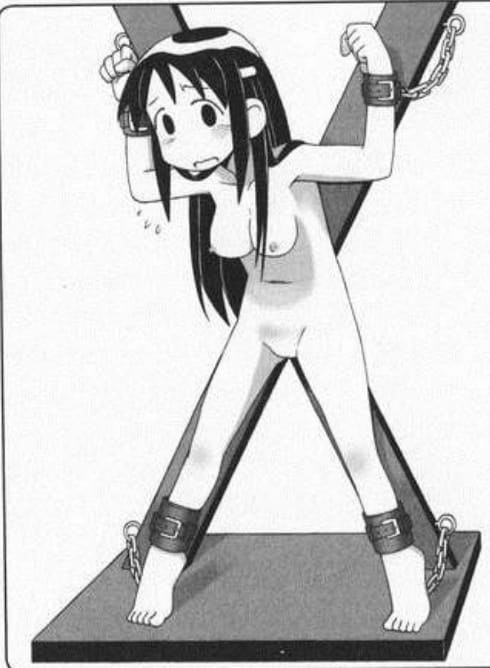
\includegraphics[width=0.6\textwidth]{Images/sm-frame.jpeg}
\caption{X型束缚架示意图}
\end{figure}

开脚束缚用的椅子，就是样子像妇科检查台那样的椅子。在性爱旅馆中，有像医院诊察室样子的屋子，在里面经常看到这种椅子。在这类的屋子里，可以一边玩医生游戏，一边将SM加入进来，所以在轻度SM阶段也是非常推荐的。

SM专用房间或者SM旅馆，是专门为SM准备的地方。里面不仅有束缚设备，而是从牢房到悬吊类的设备都有。

在这类屋子里，有平常看不到的三角木马、禁闭室，还有为了灌肠准备的排水设备。屋子也有日本和欧美风格，也有的是模仿医院和教室，可以一边SM一边玩cosplay。

在这些SM专用房间中有束缚和口球类的用具，所以空着手去也没有问题。但是这些要接触身体的道具是不是杀过菌就不清楚了，如果不放心的话可以不用。

像SM专用房间这类特殊的地方一般都有主页，去之前上去调查一下吧~

\subparagraph{适合初学者的器具的使用方法}

对于还不能用绳子进行束缚的初学者来说，SM道具是非常好的朋友。带上就可以迅速的束缚，而且也不会给人难以接受的印象，这里就介绍一下这类面向初学者的SM用具。

\paragraph{初学者的SM用具}

首先，既然是面向初学者，所以就要选择一些不会给女性带来难以接受的印象的道具。比如手铐，如果是金属制的就很容易让人联想到是中世纪的奴隶带的这样的印象。所以先从普通的选起吧~

此外SM的道具种类很多，初学者阶段还是局限在手铐、脚铐、项圈、口枷这4种比较好。这4种以外的SM道具往往是像束缚台那样大型和昂贵的东西，初学者一般也玩不起。

除了上面这4种，也有全身束缚用的道具，主要是橡胶或者皮革制成的，用一件这样的道具就可以束缚全身，而且样子也很像绳子束缚的那样。对于初学者和中级玩家来说都是可以轻松使用的道具。

\paragraph{SM道具的保养}

入手SM道具是很必要的。在SM中道具经常会沾上液体，如果之后就这样不管，不仅会让道具有臭味，还可能会损坏道具本身。

橡胶制的道具，要定期水洗，之后好好晾干后保存。金属类的道具如果有水残留在上面还会生锈。皮革制的道具，除了要清除上面的脏东西，还要定期用建材超市中皮革养护品来保养。如果水洗之后不晾干就保存是很容易发霉的。

此外，口球中会残留唾液，所以要在唾液变干之前洗干净。像这类和嘴接触的道具，要用消毒类酒精做好消毒的工作。

\paragraph{手铐、脚铐}

手铐脚镣可以说是SM道具中最有代表性的了吧。用它们可以轻松的完成束缚，所以在初学者到高级玩家中都有很高的人气。

材料主要有橡胶、皮革和金属。金属的手铐和脚铐往往给人重度的印象也不容易买到，所以先选用橡胶或者皮革的制品吧。

橡胶制的手铐脚铐很便宜，也容易清洗，沾了脏东西也容易弄掉，但是橡胶和皮肤的贴合性不好，如果夹住皮肤也会很痛，而且因为不透气，出汗会很不好受。

皮革制品要贵一些，但是和皮肤贴合性比较好，和适合长时间束缚的情况。权衡这两种类型道具的优缺点和预算，灵活选用吧~

\subparagraph{使用手铐脚铐的玩法}

只束缚手脚就足以让人兴奋了~下面就来介绍一些手脚束缚的各种玩法样式。

\paragraph{后手束缚}

这样就无法用手遮挡自己的乳房和性器官，所以很容易产生被虐感。在平躺的时候手会承受体重的压力，所以要避免压伤。

\begin{figure}[h]
\centering
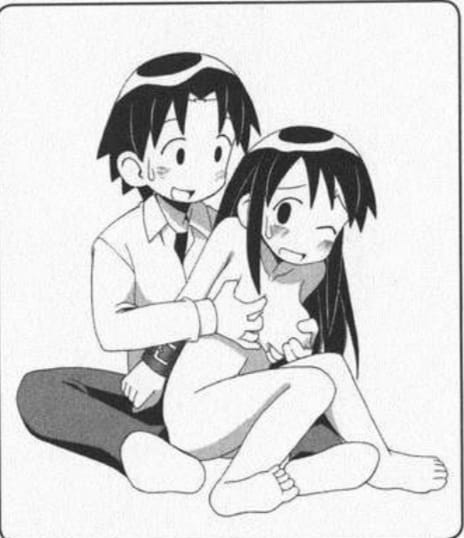
\includegraphics[width=0.6\textwidth]{Images/handcuff-back.jpeg}
\caption{后手束缚示意图}
\end{figure}

\paragraph{单手单脚束缚}

像双手抱着脚踝那样，把双手与对应一侧的脚踝束缚在一起的方式。双手也会随着双脚的分开而分开。身体正面的各处在抵抗不了的状态下被一览无余。

\begin{figure}[h]
\centering
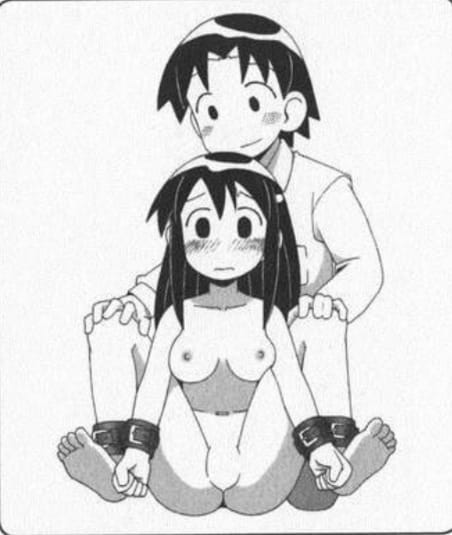
\includegraphics[width=0.6\textwidth]{Images/handcuff-single.jpeg}
\caption{单手单脚束缚示意图}
\end{figure}

\paragraph{双手双脚束缚}

就是将双手和双脚全部束缚在一起的方法。侧身躺下的话可以将性器官一览无余，非常适合对性器官的爱抚。

\begin{figure}[h]
\centering
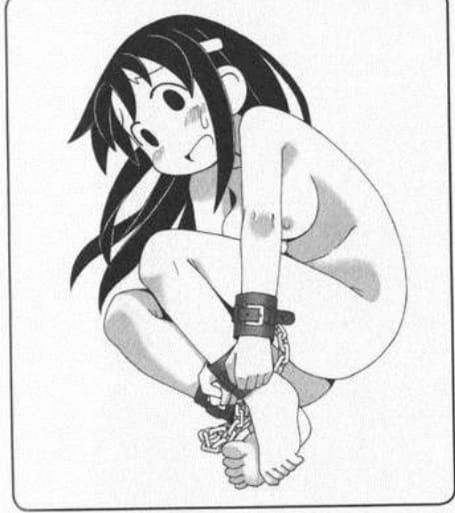
\includegraphics[width=0.6\textwidth]{Images/handcuff-double.jpeg}
\caption{双手双脚束缚示意图}
\end{figure}

\paragraph{使用支棒的束缚}

就是将金属支棒连接在手铐脚铐中的束缚方法。用支棒连接脚铐，再配合后手束缚，全身都处于无法动态的状态。

\begin{figure}[h]
\centering
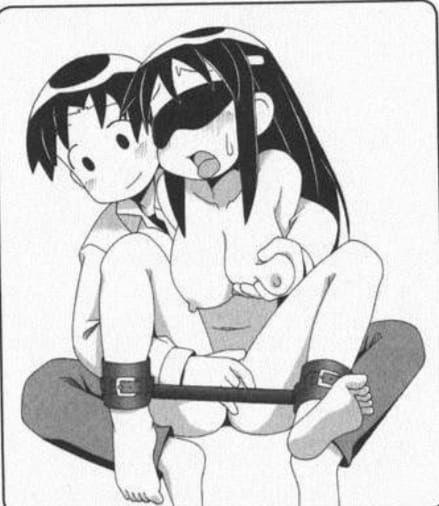
\includegraphics[width=0.6\textwidth]{Images/handcuff-rod.jpeg}
\caption{使用支棒的束缚示意图}
\end{figure}

\paragraph{项圈}

SM的标志之一就是项圈。仅仅戴上就可以有宠物的感觉，是种可以给人很强被虐感的SM道具。

虽然有专用的SM项圈，但是在女性中人气很高的是狗用的项圈。不过在这种项圈上往往涂有防虫剂，为了防止沾到身上使用前要洗干净。如果为了外观可爱而选用小型犬类用的项圈的话，要注意尺寸如果太小，戴上去会很不好受。

SM专用的项圈就没有上述的问题，立刻就可以使用，在项圈上有可以拴牵绳也可以用来固定手铐的环，如果要固定手铐的话就选用SM专用的项圈吧~

\subparagraph{双手束缚到项圈}

就是将手铐固定到有固定环的项圈上的束缚方式。这样手无法遮挡自己的身体也无法背后，很适合仰面向上的场合。不过脖子会承受手的重量，有勒住脖子的危险。

\begin{figure}[h]
\centering
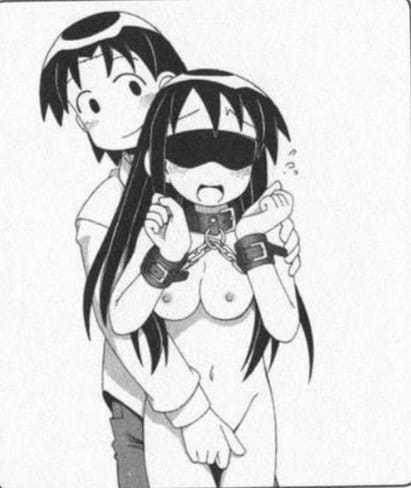
\includegraphics[width=0.6\textwidth]{Images/collar-hands.jpeg}
\caption{双手束缚到项圈示意图}
\end{figure}

	\item \textbf{性玩具}

在SM中使用性玩具，可以更加增加气氛。S可以使用玩具爱抚M，轻松的调教M。下面讲讲方法。此外，也不要仅仅使用玩具爱抚，不要忘记和其他的爱抚方式组合哦~

\subparagraph{振动器}

当然不能光使用振动器来爱抚，还要组合其他的形式。

比较有代表性的，在放入振动器的情况下，对M作出不要掉出来的指示。并且在M忍耐的时候组合打屁股的方式。

还可以在用振动器爱抚的同时，进行类似"如果你还要动得更厉害的话，就求我吧"这样的语言虐待。当然也可以用镜子让M看看自己的样子，来提升M的羞耻感。

\subparagraph{伸缩转动器}

使用的方法和振动器差不多，最大限度的利用遥控器吧。和振动器不同，可以用伸缩转动器从乳头开始爱抚身体的各个部位。利用这个特性可以对全身进行爱抚。

此外，也可以在束缚状态中把转动器放在内衣中，然后在稍微远的地方切换开关。

当然不要忘记，也可以定期把开关关掉，然后让M做出请求，或是在镜子前让M看自己的状态，提升羞耻感。

\item \textbf{打屁股}

打屁股在一般的性生活中不太会用到，但是在SM中是很普通的事情。打屁股不需要特殊的道具，只要手就可以。而且喜欢屁股被打的M也是比较多的，所以尽可能尝试一下吧~

当然，不是打下去就好了。在轻度SM阶段只要打屁股就好了。打屁股以外的地方很容易感到痛，但是屁股不那么容易觉得痛。

关于打的方法，也不仅仅是用力，而是要尽量用手心打出声音来。也不要频率不变，而要强弱交换，时停时始。

在打完一阵后，可以用手指轻抚变得敏感的皮肤，用指尖像挠痒一样的效果很不错。

打的部位也不要局限在屁股的一个地方，可以时不时的用指尖触碰阴道，将感觉传遍全身。

此外，打的时候也不要忽然就打，在其他的爱抚中打屁股的比较好。比较有代表性的有下面这两种。

\subparagraph{做爱的时候}

就是在以坐式或者后入式方式做爱的时候打屁股。

或者命令M扭动腰部，在扭动变慢的时候打屁股也不错。

\subparagraph{用玩具爱抚的时候}

在放入振动器并命令不要掉出来的状态下打屁股。

此外，在放入伸缩转动器的状态下，不断切换开关，并且一边打屁股的方式也是很流行的。
\end{enumerate}

\textit{【编者注】}轻度SM的核心在于建立信任和探索边界，而非追求强烈的感官刺激。建议从非侵入性的方式开始，注重沟通和反馈，让双方在安全舒适的氛围中逐渐探索。

\section{SM的安全入门指南}

虽说对SM有兴趣，但各种SM形式进行的方法和步骤却不是那么好懂，常常让人不知道从哪里入手。而且在SM束缚的过程中也有受伤的危险——如果不掌握正确的知识和方法，SM就可能变成危险的活动。

以下是从入门到实践的逐步指导原则：

\noindent\textbf{第一步：沟通与说服伴侣}

\begin{enumerate}
	\item 坦诚表达自己的兴趣——用非威胁性的方式描述SM对你的吸引力
	\item 了解对方的边界和兴趣范围——可以一起阅读入门书籍或观看教育类资料
	\item 从最轻微的形式开始尝试——不要一开始就追求高强度体验
	\item 接受对方可能需要时间来理解和接受——不要施加压力
\end{enumerate}

\noindent\textbf{第二步：学习基础安全知识}

\begin{itemize}
	\item \textbf{安全词（Safeword）}：约定一个明确的停止信号（如"红色=立即停止""黄色=减速"），确保在任何状态下都能被识别和使用
	\item \textbf{束缚安全}：避免压迫颈部/关节；绳子不应阻断血液循环（检查手指颜色和温度）；剪刀常备在手边以便紧急剪断
	\item \textbf{器具卫生}：所有接触皮肤或黏膜的工具使用前后必须彻底清洁消毒
	\item \textbf{身体禁区}：明确哪些部位绝对不能触碰或施加压力（如眼睛、颈椎、内脏器官区域）
\end{itemize}

\noindent\textbf{第三步：循序渐进的实践}

\begin{itemize}
	\item 从轻拍、羽毛抚摸等低强度感觉开始
	\item 逐步尝试简单的手腕束缚（使用专门设计的束带而非粗糙绳索）
	\item 每次活动后进行"\textbf{事后关怀（Aftercare）}"——拥抱、交谈、确认对方状态良好
	\item 定期回顾和讨论双方的感受，不断调整和改进
\end{itemize}



\section{性爱旅馆与 SM 场所的使用}

又要准备道具，又要有SM的氛围，所以立刻就进行SM往往比较困难。

不过，在性爱旅馆中既准备好了SM用的道具，又有SM的氛围，所以在轻度SM阶段，充分利用性爱旅馆中的设备也是一个办法。

性爱旅馆中的SM房间，有的只是普通的房间放入了SM的装备，有的是在建造的时候就是为了SM准备的。

这两种都没问题，但是如果去专门的SM房间或者专门的SM旅馆的话，就没法用“碰巧这个屋子里有SM装备，那我们就试试看吧”这个理由来当做尝试的借口了。

所以如果对方对SM有些抵抗的话，还是从有SM装备的普通性爱旅馆开始吧。

比较有代表性的SM装备有手脚束缚用的铐具和架子、开脚束缚的椅子。

手脚束缚的铐具很多都连在床上，是为了在床上“大”字形束缚用的。束缚架中最流行的是四段有手铐脚铐的“X”型木架。

不止在SM旅馆中，普通的性爱旅馆中也有这种架子，往往是粉红色的，看上去很容易就让人接受，所以非常推荐在轻度SM阶段使用。开脚束缚用的椅子，就是样子像妇科检查台那样的椅子。

在性爱旅馆中，有像医院诊察室样子的屋子，在里面经常看到这种椅子。

在这类的屋子里，可以一边玩医生游戏，一边将SM加入进来，所以在轻度SM阶段也是非常推荐的。SM专用房间或者SM旅馆，是专门为SM准备的地方。

里面不仅有束缚设备，而是从牢房到悬吊类的设备都有。

在这类屋子里，有平常看不到的三角木马、禁闭室，还有为了灌肠准备的排水设备。

屋子也有日本和欧美风格，也有的是模仿医院和教室，可以一边SM一边玩cosplay。

在这些SM专用房间中有束缚和口球类的用具，所以空着手去也没有问题。

但是这些要接触身体的道具是不是杀过菌就不清楚了，如果不放心的话可以不用。

\noindent\textit{【编者注】}使用公共场所的共享器具前应确认清洁状况，不放心时可自备或不用；自带的束缚器械须检查稳固性与快速释放功能，避免单人独处时做需要他人才能解开的束缚。
\textit{【编者注】}关于SM入门的系统化学习资源，推荐参考三叶所著《私の体、私の心 —— YOUAREMINE！！》（一迅社，2014）。该书从说服伴侣开始，到各类SM形式的步骤和注意点，将必要知识逐步教授给初学者，是目前日文领域较为系统的SM入门教材之一。

\chapter{进阶实践与健康安全}

本章是本卷实践内容的安全技术核心：SM 的核心元素与常见活动的技术要点和风险、全面的安全措施、绳缚的神经与循环安全、电击与夹具类玩具的使用细则，以及高强度场景后的情绪跌落照护。进阶不等于冒险——每前进一步，安全知识都应先于技巧一步。


\section{SM 的定义、核心元素与常见活动}

SM是Sadomasochism的缩写，指的是一种包含支配-服从、施虐-受虐元素的性偏好或性行为方式。SM涉及两个主要角色：S（Sadist，施虐者）和M（Masochist，受虐者）。

1. \textbf{核心元素}：
  \begin{itemize}
  \item \textbf{支配与服从（D/S）}：
    \begin{itemize}
    \item \textbf{心理动力}：支配者在控制中获得满足，服从者在放弃控制中获得放松和安全感。这种权力交换可以满足双方的心理需求，如自我实现、被保护感或责任感
    \item \textbf{实践细节}：
      \begin{itemize}
      \item 权力动态的协商：明确双方期望的权力程度和范围
      \item 角色的具体表现：语言命令、身体姿势、行为限制等
      \item 信任的建立：长期的D/S关系需要高度的信任和情感连接
      \item 权力的责任：支配者对服从者的安全和福祉负有责任
      \end{itemize}
    \end{itemize}
  \item \textbf{痛苦与快乐（S/M）}：
    \begin{itemize}
    \item \textbf{心理动力}：痛苦与快乐在SM中是复杂的交织关系。疼痛可以释放内啡肽（天然的愉悦激素），创造强烈的身体和情感体验。对于一些人，疼痛是一种集中注意力、释放压力或体验极限的方式
    \item \textbf{实践细节}：
      \begin{itemize}
      \item 疼痛阈值的探索：逐渐增加刺激强度，了解彼此的承受能力
      \item 疼痛的类型和部位：不同类型的疼痛（如刺痛、鞭打、压迫）在不同部位会产生不同的体验
      \item 疼痛与愉悦的转化：通过心理状态和情境设置，将疼痛转化为愉悦体验
      \item 个体差异：每个人对疼痛的感受和反应都不同，需要充分沟通
      \end{itemize}
    \end{itemize}
  \item \textbf{契约与边界}：
    \begin{itemize}
    \item \textbf{心理动力}：明确的契约和边界为SM互动提供安全感，让双方能够在安全的框架内探索。这种结构化的互动可以减少焦虑，增强信任
    \item \textbf{实践细节}：
      \begin{itemize}
      \item 书面或口头契约：详细列出双方的权利、责任、偏好和限制
      \item 边界的类型：硬性边界（绝对不允许）和软性边界（可以考虑）
      \item 边界的动态性：边界可能随时间变化，需要定期重新协商
      \item 契约的执行：双方都有责任遵守约定的规则，尊重彼此的边界
      \end{itemize}
    \end{itemize}
  \end{itemize}

2. \textbf{常见活动}：
  \begin{itemize}
  \item \textbf{捆绑（Bondage）}：
    \begin{itemize}
    \item 描述：使用绳索、手铐、皮带等工具限制身体自由，创造束缚感。捆绑可以是简单的手腕束缚，也可以是复杂的绳艺图案，如日本绳缚（Shibari）或西方绳缚（Western Bondage）
    \item 绳索技术：
      \begin{itemize}
      \item \textbf{单柱绑（Single Column Tie）}：最基础的绑法，用于固定单个肢体（如手腕或脚踝）
        \begin{itemize}
        \item 步骤：将绳索绕过肢体2-3圈，然后做一个半结固定，再打一个安全结
        \item 安全要点：保持绳索松紧适度，能插入1-2根手指为宜
        \end{itemize}
      \item \textbf{双柱绑（Double Column Tie）}：用于固定两个肢体（如双手手腕、双脚脚踝或手腕与脚踝）
        \begin{itemize}
        \item 步骤：将绳索先在一个肢体上做单柱绑，然后绕过另一个肢体，形成八字形缠绕，最后固定
        \item 安全要点：确保两个肢体受力均匀，避免过度拉伸关节
        \end{itemize}
      \item \textbf{胸衣绑法（Chest Harness）}：围绕胸部的绑法，可增强胸部线条或限制上半身活动
        \begin{itemize}
        \item 步骤：从背部开始，绳索穿过腋下，在胸前交叉，再回到背部固定
        \item 安全要点：避开乳房敏感区域，避免压迫胸腔影响呼吸
        \end{itemize}
      \item \textbf{日式绳缚基础（Basic Shibari）}：
        \begin{itemize}
        \item 特点：注重美学和艺术性，常用菱形或方形图案
        \item 安全要点：学习专业的绳缚课程，了解人体解剖学，避免压迫神经和血管
        \end{itemize}
      \item \textbf{进阶绳缚技术}：
        \begin{itemize}
        \item \textbf{复杂绳缚图案}：
          \item 龟甲绑（Kikkou）：胸部或背部的菱形图案，需要精确的绳索排列
          \item 蛛网绑（Kumo）：类似蜘蛛网的复杂图案，覆盖更大面积
        \item \textbf{悬挂捆绑安全要点}（需专业指导）：
          \item 学习专业课程：悬挂捆绑需要专业知识和技能，不建议自学
          \item 设备要求：使用专业的悬挂点和安全设备，确保承重能力
          \item 承重分布：将重量均匀分布在多个支撑点，避免单点承重
          \item 姿势选择：避免压迫内脏和重要血管，选择安全的悬挂姿势
        \item \textbf{进阶安全考虑}：
          \item 学习解剖学：深入了解人体结构，特别是神经和血管的位置
          \item 练习和经验：在专业指导下逐步练习，积累经验
          \item 应急准备：制定详细的应急计划，包括如何快速解除复杂捆绑
          \item 定期检查：定期检查绳索和设备的状况，确保安全使用
        \end{itemize}
      \end{itemize}
    \item 工具类型：
      \begin{itemize}
      \item \textbf{绳索}：
        \begin{itemize}
        \item \textbf{天然纤维绳索}：
          \item \textbf{麻绳}：
            \item 特点：传统且常用，质地粗糙，摩擦力大，易于打结和调整
            \item 优点：透气性好，吸汗性强，适合长时间使用
            \item 缺点：需要定期保养（上油），易磨损
            \item 适用场景：日式绳缚（Shibari）的首选材料
          \item \textbf{黄麻}：
            \item 特点：比麻绳更柔软，颜色浅黄，质地细腻
            \item 优点：摩擦力适中，易于操作，适合初学者
            \item 缺点：强度略低于麻绳
            \item 适用场景：日式绳缚和西方绳缚的基础练习
          \item \textbf{棉绳}：
            \item 特点：非常柔软，触感舒适，颜色多样
            \item 优点：对皮肤友好，适合敏感肌肤，不易造成勒痕
            \item 缺点：强度较低，易打滑，吸水性强（湿水后易拉伸）
            \item 适用场景：温柔的捆绑、初学者练习、敏感部位捆绑
        \item \textbf{合成纤维绳索}：
          \item \textbf{尼龙绳}：
            \item 特点：强度高，光滑耐用，颜色丰富
            \item 优点：不易磨损，易于清洁，湿水后强度不变
            \item 缺点：摩擦力小，易打滑，透气性差
            \item 适用场景：西方绳缚、快速捆绑、户外场景
          \item \textbf{聚酯绳}：
            \item 特点：类似尼龙绳，但更硬，熔点更高
            \item 优点：强度高，耐高温，不易变形
            \item 缺点：触感较硬，透气性差
            \item 适用场景：特殊场景捆绑、需要高强度的捆绑
        \end{itemize}
      \item \textbf{金属工具}：
        \begin{itemize}
        \item \textbf{手铐}：
          \item 类型：普通手铐、可调节手铐、软边手铐
          \item 安全要点：选择有快速释放功能的手铐，避免使用一次性手铐；定期检查锁具功能；避免长时间佩戴导致血液循环问题
          \item 风险提示：避免过度收紧，防止手腕神经损伤
        \item \textbf{脚镣}：
          \item 类型：普通脚镣、带链条脚镣、可调节脚镣
          \item 安全要点：确保链条长度适中，避免绊倒；定期检查脚踝处皮肤状况
          \item 风险提示：避免长时间佩戴，防止脚踝肿胀和神经损伤
        \item \textbf{项圈}：
          \item 类型：皮革项圈、金属项圈、可调节项圈
          \item 安全要点：选择有安全扣的项圈，避免使用带锁且无钥匙的项圈；确保能插入2-3根手指
          \item 风险提示：避免压迫颈部动脉和气管，防止窒息风险
        \end{itemize}
      \item \textbf{辅助工具}：
        \begin{itemize}
        \item \textbf{束缚带}：
          \item 类型：魔术贴束缚带、带扣束缚带、可调节束缚带
          \item 安全要点：选择宽度足够的束缚带（至少5cm），避免局部压力过大；确保有快速释放功能
          \item 适用场景：初学者使用，快速捆绑，温柔场景
        \item \textbf{分腿器}：
          \item 类型：固定角度分腿器、可调节分腿器
          \item 安全要点：选择重量适中的分腿器，避免使用过重导致关节损伤；确保底部有防滑设计
          \item 风险提示：避免过度打开双腿，防止髋关节损伤
        \item \textbf{眼罩}：
          \item 类型：柔软眼罩、皮革眼罩、带填充眼罩
          \item 安全要点：确保透气性良好，避免长时间佩戴；选择有快速释放功能的眼罩
          \item 作用：增强其他感官体验，增加神秘感
        \item \textbf{口塞}：
          \item 类型：硅胶口塞、橡胶口塞、带孔口塞
          \item 安全要点：选择大小合适的口塞，确保佩戴者能正常呼吸；使用前消毒；定期检查佩戴者状态
          \item 风险提示：避免使用无孔口塞，防止窒息风险；避免长时间佩戴导致口腔肌肉疲劳
        \end{itemize}
      \end{itemize}
    \item 安全注意事项：
      \begin{itemize}
      \item 避开动脉和神经密集区域（如手腕内侧的桡动脉、颈部的颈动脉、大腿内侧的股动脉）
      \item 定期检查血液循环（每15-20分钟检查一次肢体颜色、温度和麻木感）
      \item 学习正确的捆绑技术，特别是日本绳缚（Shibari）的安全要点
      \item 确保有快速解除捆绑的工具（如专门的安全剪刀，放在容易拿到的地方）
      \item 建立安全词或安全信号，确保参与者可以随时停止
      \end{itemize}
    \item 生理和心理考虑因素：
      \begin{itemize}
      \item \textbf{身体状况评估}：
        \begin{itemize}
        \item 事前沟通：了解参与者的健康状况，特别是心血管疾病、糖尿病、关节炎、神经疾病等慢性疾病
        \item 肢体检查：检查是否有伤口、淤青、肿胀或皮肤过敏情况
        \item 特殊情况：孕妇、老年人、有慢性疾病者应避免高强度捆绑
        \end{itemize}
        \begin{itemize}
        \item 角色确认：明确支配者（Top）和服从者（Bottom）的角色期望和边界
        \item 信任建立：确保双方有足够的信任和沟通基础
        \item 情绪状态：避免在情绪不稳定时进行捆绑活动
        \end{itemize}
      \item \textbf{角色心理需求}：
        \begin{itemize}
        \item 支配者（Top）：需要承担责任，关注服从者的安全和感受
        \item 服从者（Bottom）：需要感到安全和被照顾，建立安全感
        \end{itemize}
      \end{itemize}
    \item 场景设计：
      \begin{itemize}
      \item \textbf{基础场景}：
        \begin{itemize}
        \item 手腕束缚：简单地将双手绑在前面或后面
        \item 床上束缚：使用束缚带或绳索将四肢固定在床的四角
        \end{itemize}
      \item \textbf{进阶场景}：
        \begin{itemize}
        \item 站立捆绑：将双手绑在头顶，双脚分开固定
        \item 椅子捆绑：将身体固定在椅子上，限制活动
        \end{itemize}
      \item \textbf{创意场景}：
        \begin{itemize}
        \item 悬挂捆绑（需专业指导）：使用滑轮或固定点将身体部分悬挂
        \item 组合场景：结合感觉剥夺（眼罩）和感觉增强（羽毛、冰块）
        \end{itemize}
      \end{itemize}
    \item 事后护理：
      \begin{itemize}
      \item \textbf{物理护理}：
        \begin{itemize}
        \item 缓慢解除捆绑：避免快速释放导致血压波动
        \item 检查身体状况：检查是否有勒痕、淤青或麻木区域
        \item 恢复血液循环：轻轻按摩捆绑部位，促进血液循环
        \item 补水和营养：提供水和轻食，补充能量
        \end{itemize}
      \item \textbf{心理护理}：
        \begin{itemize}
        \item 情感支持：给予拥抱、赞美和肯定
        \item 沟通反馈：询问感受，分享体验
        \item 休息时间：确保有足够的时间恢复情绪和体力
        \end{itemize}
      \item \textbf{后续观察}：
        \begin{itemize}
        \item 24小时内观察身体状况：如果出现持续麻木、肿胀或疼痛，应及时就医
        \item 情绪支持：后续几天保持沟通，确保情绪稳定
        \end{itemize}
      \end{itemize}
    \item 风险提示：神经损伤、血液循环障碍、窒息、关节损伤、心理创伤
    \end{itemize}
  \item \textbf{鞭打（Flagellation）}：
    \begin{itemize}
    \item 描述：使用鞭子、皮鞭、藤条等工具对身体进行有控制的抽打
    \item 工具类型：马鞭、皮鞭、藤条、拍子、散鞭等
    \item 安全注意事项：
      \begin{itemize}
      \item 避开头部、脊柱、关节、肾脏等敏感部位
      \item 从较轻的力度开始，逐渐增加强度
      \item 了解不同工具的使用方法和安全区域
      \item 保持工具清洁，避免感染
      \end{itemize}
    \item 风险提示：皮肤损伤、瘀伤、肌肉损伤、感染
    \end{itemize}
  \item \textbf{角色扮演（Role-playing）}：
    \begin{itemize}
    \item 描述：扮演特定角色进行情境互动，增强性体验
    \item 常见角色组合：主人与奴隶、教师与学生、医生与病人、警察与犯人等
    \item 安全注意事项：
      \begin{itemize}
      \item 明确角色边界和现实边界
      \item 协商角色的行为范围和限制
      \item 设定场景的开始和结束信号
      \item 尊重彼此的情感反应，避免真实伤害
      \end{itemize}
    \item 风险提示：情感混淆、边界模糊、心理创伤
    \end{itemize}
  \item \textbf{感觉剥夺（Sensory deprivation）}：
    \begin{itemize}
    \item 描述：使用眼罩、耳塞、头套等工具限制视觉、听觉或其他感官
    \item 工具类型：眼罩、耳塞、隔音耳机、头套、布袋等
    \item 安全注意事项：
      \begin{itemize}
      \item 确保环境安全，避免参与者受伤
      \item 定期检查参与者的情绪状态
      \item 不要长时间剥夺感官（一般不超过1小时）
      \item 确保参与者可以随时沟通
      \end{itemize}
    \item 风险提示：焦虑、恐慌、迷失方向
    \end{itemize}
  \item \textbf{感觉增强（Sensory enhancement）}：
    \begin{itemize}
    \item 描述：使用各种工具增强身体的感觉体验
    \item 工具类型：羽毛、冰块、热蜡、按摩油、振动器等
    \item 安全注意事项：
      \begin{itemize}
      \item 测试工具的温度和刺激强度
      \item 避开敏感部位（如眼睛、黏膜）
      \item 确保工具清洁，避免感染
      \item 尊重参与者的反应
      \end{itemize}
    \item 风险提示：烫伤、冻伤、过敏反应
    \end{itemize}
  \item \textbf{羞辱（Humiliation）}：
    \begin{itemize}
    \item 描述：通过语言或行为进行有控制的羞辱，满足心理需求
    \item 表现形式：语言羞辱、身体姿势羞辱、任务羞辱等
    \item 安全注意事项：
      \begin{itemize}
      \item 明确羞辱的边界和类型（如身体羞辱、能力羞辱）
      \item 避免触及参与者的真实痛点和创伤
      \item 保持羞辱的虚构性，避免现实伤害
      \item 确保事后有充分的情感支持
      \end{itemize}
    \item 风险提示：自尊心伤害、心理创伤、关系破裂
    \end{itemize}
  \item \textbf{温度 play（Temperature play）}：
    \begin{itemize}
    \item 描述：使用冷热物品刺激身体，创造温度变化的快感
    \item 工具类型：冰块、热蜡、温毛巾、低温蜡烛等
    \item 安全注意事项：
      \begin{itemize}
      \item 测试物品的温度，避免烫伤或冻伤
      \item 选择专门的低温蜡烛（熔点在50-60℃）
      \item 避免将热蜡滴在敏感部位（如眼睛、黏膜、乳头）
      \item 不要将冰块直接放在皮肤上过长时间
      \end{itemize}
    \item 风险提示：烫伤、冻伤、皮肤过敏
    \end{itemize}
  \item \textbf{呼吸控制（Breath play）}：
    \begin{itemize}
    \item 描述：通过控制呼吸获得强烈的身体体验（属于边缘活动，风险较高）
    \item 方式：手部压迫、绳索勒颈、塑料袋等
    \item 安全注意事项：
      \begin{itemize}
      \item 仅在双方充分了解风险并具备急救知识的情况下进行
      \item 始终保持对参与者的密切观察
      \item 设定明确的安全词和停止信号
      \item 避免单独进行，确保有第三者在场
      \end{itemize}
    \item 风险提示：窒息、脑损伤、死亡（极端风险）
    \end{itemize}
  \item \textbf{穿刺 play（Needle play）}：
    \begin{itemize}
    \item 描述：使用无菌针具在身体表面进行有控制的穿刺，创造独特的感觉体验
    \item 工具类型：一次性无菌针、穿刺针、穿孔工具等
    \item 安全注意事项：
      \begin{itemize}
      \item 仅使用一次性无菌针具，避免感染
      \item 避开重要血管、神经和内脏器官
      \item 学习正确的穿刺技术和消毒方法
      \item 穿刺后保持伤口清洁，避免感染
      \end{itemize}
    \item 风险提示：感染、出血、神经损伤、过敏反应
    \end{itemize}
  \item \textbf{性玩具使用（Toy play）}：
    \begin{itemize}
    \item 描述：使用专门的SM性玩具进行刺激和控制
    \item 工具类型：振动器、电击器、乳头夹、阴蒂刺激器、前列腺按摩器等
    \item 安全注意事项：
      \begin{itemize}
      \item 选择高质量、安全材质的玩具（如硅胶、不锈钢）
      \item 了解玩具的使用方法和安全限制
      \item 定期清洁和消毒玩具
      \item 避免过度刺激，注意身体反应
      \end{itemize}
    \item 风险提示：机械损伤、电击伤、过敏反应、感染
    \end{itemize}
  \item \textbf{奴役训练（Training）}：
    \begin{itemize}
    \item 描述：通过设定规则和任务，训练服从者的行为和反应
    \item 常见训练内容：姿势训练、语言回应训练、服务训练、纪律训练等
    \item 安全注意事项：
      \begin{itemize}
      \item 设定明确的训练目标和时间范围
      \item 避免过度训练，注意身体和心理极限
      \item 提供积极的反馈和奖励机制
      \item 确保训练内容符合双方的边界和意愿
      \end{itemize}
    \item 风险提示：心理压力、身体疲劳、情感伤害
    \end{itemize}
  \item \textbf{仪式与崇拜（Ritual  Worship）}：
    \begin{itemize}
    \item 描述：通过特定的仪式和行为表达崇拜和敬意
    \item 常见形式：跪礼、吻脚、身体崇拜、物品崇拜等
    \item 安全注意事项：
      \begin{itemize}
      \item 明确仪式的意义和边界
      \item 避免真实的贬低和侮辱
      \item 确保仪式的自愿性和尊重性
      \item 设定仪式的开始和结束信号
      \end{itemize}
    \item 风险提示：自尊心伤害、心理创伤、边界模糊
    \end{itemize}
  \end{itemize}


\section{组合玩法与场景编排}

\noindent\textit{【编者注】}以下玩法强度高于轻度入门，尝试前应先约定安全词、NG 清单与事后照护（参见本卷相关各节）。

组合玩法的方法和种类大家都知道，在SM中有束缚、羞辱等各式各样的玩法。

当然，每种玩法独立的来说都是十分有趣的，不过如果可以把几种玩法组合在一起，就能让M感受到更强的被虐感和羞耻心。

下面，就来介绍一下这种组合的方式和种类，还有爱抚的方法。

首先，来说说组合玩法的种类。

就像在普通的性爱中可以一边插入一边爱抚乳房那样，在SM中混合各种各样的玩法是很普通的。

并且SM本身就是比普通性爱更加强调嗜好的一种方式，不同的嗜好有不同的玩法，所以SM玩法有容易组合的一面。

一般来说，就是将爱抚、插入这些普通的性爱方式，和SM中束缚、语言虐待、羞辱这些伴随着痛苦的方式混合在一起。

特别是，作为SM中很重要的概念，一定要组合出激发羞耻心和被虐心的玩法。

下面介绍几种有代表性的方式。 1.侍奉+束缚或语言虐待这种方式在SM中很有代表性。

就是在束缚或者语言虐待的同时，口交或者舔身体。

在这种束缚的状态下侍奉S，有很强的被虐实感。

舔身体也包括舔手或脚，如果是脚的话，要注意卫生哦～ 2.束缚+爱抚就是在束缚状态下的爱抚。

在身体的自由被剥夺的状况下爱抚，对M来说有非常大的被虐感。SM中的爱抚不只限于用手，作为SM的特征，使用玩具的时候也很多。 3.打屁股+爱抚就是在打屁股的同时爱抚。

很多M都希望感受痛和性爱这两方面的快感，这种方式就非常有效果。

也有在性器官中插上玩具，在命令M不要让它掉下来的同时打屁股。 4.束缚+插入就是在束缚的状态下做爱。

双方是恋人关系的话，果然最后多数还是会以做爱结束的吧。

在束缚状态下插入，女性逃脱不了，有很强的被侵犯一样的被虐感。 5.束缚+放置放置本身就可以给予M被虐感。

这时候再加上束缚的话就可以更加增强这种感觉。

在放置同时用玩具固定乳头或性器官也是很很流行的。

不过，并不是每一个人都喜欢这种方式，所以玩之前一定要和对方确认哦。

在放置的同时，不要忘记时刻确认M的状态，放置M受伤。 6.玩法+镜子在各种各样的玩法同时使用镜子也是很常见的一种方式。

让M看到自己在镜中丢人的样子，可以给予很大的羞耻心。

特别是紧缚或者使用全身束缚道具、口球这种场合，让M在镜中确认自己的姿态，可能会给M相当大的羞耻心。

\section{侍奉类玩法}

侍奉玩法，如同字面意思，就是M侍奉S的玩法。

在普通的性爱当中，也有口交这种相互侍奉的方式。

在SM中的侍奉，终归是让M感受到被虐感的侍奉方式。

正因为有这样的区别，SM中的侍奉不仅仅是舔性器官，也包括了脚、肛门甚至全身。

此外，SM中的侍奉往往混合了束缚或者羞辱，这也是特征之一。

下面就来介绍一下各种各样的侍奉方式。 

\subsection{口交}

当然，不仅仅是口交而已，而是比如在束缚状态下命令或是要求M来舔。

这个时候，M在束缚状态下手和身体都动不了，多少做得有点笨拙，看着M那努力的样子，心中一定充满爱意吧。

温柔的注视M吧～如果希望在口交中使用双手的话，那么可以把双手束缚在前面。

此外，女性在束缚状态下口交时，长发有时会跑到嘴里或者眼睛里，所以时不常的帮M拨动一下头发比较好。

同时也要注意阴茎如果进入到喉咙深处的话可能会让M呛到。口交中的爱抚，比较有代表性的为是，在使用项圈的时候，有点强迫似的把M拉过来，之后在口交中揉捏M的乳头或者打屁股，还有在插入振动器并且不让它掉下来的状态中让M来口交之类的方式。

还可以在M的下面固定上旋转棒后口交， M在旋转棒的刺激性下动作会变得僵硬，在这个时候关掉旋转棒的开关，这样也是种很有效果的玩法。

此外，也有使用道具强制让M的嘴张开，强迫M进行口交的方式，不过这样让喉咙塞住的可能性很高，虽说也有喜欢这种方式的人，但是还是尽可能不要触及喉咙深处吧～ 

\subsection{舔全身}

就是在侍奉中让M舔男方乳头或身体的方式。

虽说这种方式对于S来说也不是每个人都喜欢，但是对于M来说，比起舔肛门或者脚之类，要容易接受得多。

一般舔的部位为乳头、腹部、睾丸等等。

这个时候，双手束缚在背后的M骑在S身上，很不容易保持身体的平衡，所以S不要忘记扶一下M的身体哦～当然，也不要忘记可以同时爱抚M的性器官或者用玩具爱抚M。 

\subsection{舔肛门}

这种侍奉的方式是SM中所独有的。

对于初学者来说多少会觉得有些不可接受，不过作为侍奉玩法的一种，喜欢这种方式的M也很多。

在让M舔之前一定要在洗澡的时候洗干净肛门区域，以免感染杂菌。

舔的时候S一般是仰面向上的姿势， M从口交开始慢慢向肛门侧转移。

当然，在第一次舔之前，一定要对M说：如果你不喜欢的话我也不会强迫你哦～

\section{束缚状态下的爱抚}

在SM中的束缚往往要持续很长时间，所以这之间的爱抚就变得很重要了。

这里介绍一下束缚状态下的爱抚方法。

当然在束缚状态下其他的SM方式（打屁股、语言虐待、羞辱）也要记得混合起来一起使用。

此外，束缚中插入也在这里顺便介绍一下。 

\subsection{乳房的爱抚}

束缚状态和乳房的爱抚有很强的联系。

在把双手束缚到背后，或者双手被束缚在项圈上的时候，不论怎么爱抚M都无法抵抗.仅仅是这种状态本身就可以给M很大的被虐感和羞耻感。在这种状态下的爱抚，基本上是在普通性爱中的爱抚中，再加上SM中的一些伴随着疼痛的爱抚方式。

这种伴随着疼痛的爱抚不仅仅是用手指揉捏乳头，也常常使用木夹子和榨乳机，这种使用道具让痛苦持续的方法在SM中很普遍。

在使用道具的时候，为了不超过M痛苦的极限，一定要事先决定好Give up Sign。

此外，如果使用夹子，在夹子刚刚拿下来之后，乳头部位是非常敏感的，所以这时温柔的抚摸比较好。

当然对乳头爱抚的同时进行爱抚性器官、打屁股、语言虐待也是很有效果的。 

\subsection{性器官的爱抚}

束缚状态下的性器官爱抚大致分为两类，一种是用手或者嘴的爱抚方式，一种是使用玩具的爱抚方式。

用手或嘴的方式与普通性爱中相同，不要忘记同时进行语言虐待或者让M在镜中看自己的样子这类激发羞耻心的方式。

此外，把脚M字固定之后可以让爱抚相当轻松，可以从后方同时爱抚乳房和性器官。

使用玩具的爱抚也可以和遮眼睛一起用，让M听到马达的声音，一边给M造成这种不知道接下来要爱抚哪里紧张而兴奋的感觉，一边来爱抚。

不遮眼睛的时候，也可以边让M在镜子中看自己的样子，边用玩具爱抚、打屁股或是语言虐待。

此外，将振动器或是旋转棒用道具固定在性器官上，在这样的状态下让M散步、强制口交，或是保持直立的姿势不动，都是很有效果的爱抚方式。 

\subsection{束缚中的插入}

在最后进行束缚中的插入行为来完成整个SM过程很常见。

最理想的束缚状态下的插入体位，是男性在下，M紧贴在上的骑乘位。

这种姿势不容易给M身体带来负担，可以长时间的享受进出的快感。如果使用女下男上的正常位的话，要注意M被束缚的双手会被压在背后，可能会造成发麻或留下痕迹。

如果使用后入式的话，要注意这个时候M的脸是完全贴在地上或床单上的，所以如果在床以外的地方使用这种方式，不要忘记在M的脸下面垫上毛巾之类柔软的东西。

\section{性玩具的使用}

\subsection{性玩具适合 SM 吗？}

在SM中使用玩具比在普通的性爱中要更甚。

使用玩具的话，可以进行比在普通性爱中更长时间的爱抚。

特别是S手握开关，在稍远的地方忽然打开或关闭这种的玩法也可以轻易做到。

玩具可以在一些姿势中，爱抚到用手很难爱抚到的地方。

也可以在固定玩具给予M快感的同时，再进行戴上项圈模仿小狗或是侍奉的玩法。

所以对SM来说，玩具是非常好用的道具。

\section{挑逗与放置}

\subsection{挑逗}

挑逗和放置也是在SM中一般的玩法。

所谓挑逗就是通过爱抚挑逗起M的兴奋的状态，并在恰到好处的时候忽然停止的玩法。

放置既是在束缚状态的放置不管玩法。

这两种都是让M长时间忍受的玩法，让M忍受的方式各式各样。

下面就来介绍一下这两种玩法。 挑逗玩法一般就是爱抚到非常舒服的时候忽然停止，之后再重复这个过程。

爱抚的方式不仅可以用手，也可以用玩具产生这种断断续续的感觉。

不过这种玩法不是每个女性都喜欢。

也要注意，挑逗过头儿会让气氛变坏，相反挑逗得不够有可能会让整个过程早早结束。

人与人之间的感觉差别很大，所以挑逗的时候要仔细的观察对方的表情和声音，也要在SM以外的时间聆听对方的感受。

此外，也有通过持续的爱抚来挑逗的玩法，就是在爱抚的时候，不碰性器官和乳头，持续的爱抚其他的部位，直到M忍受不了的时候再去爱抚乳头和性器官。

在这些玩法中加进遮眼睛，让M不知道接下来要触摸哪里，还可以让兴奋感再上升一个更次。

让M听到玩具电机的声音，之后忽然接触性器官也会给M带来意外的兴奋感。

也有在插入途中，突然停止抽插的动作，然后让M自己动，这种既是语言虐待又是挑逗的方式。

适度的挑逗对M来说是非常大的兴奋材料，在SM中间歇的加进来吧～ 

\subsection{放置}

如同字面意义上所说，就是放置不管的玩法。

主要是束缚状态下的放置，给M孤独感和恐惧感是一般的形式。

不过，人们对这种放置的方式的喜好也趋向两个极端。

特别是，希望S调教自己，这种类型的M不是很喜欢放置的玩法。

所以在之前一定要了解对方对放置玩法的喜好。也有的人在M被放置的时候出门，离开M的身边，这种在M束缚状放置的时候出门的方式很容易造成受伤或事故，是非常危险的。

所以目光一定不要离开M哦～如果是为了给M孤独感的话，可以把M的眼睛遮住，然后悄悄的离开到可以看到M的地方就可以了。

具体的放置玩法的方式还有，在床上翻滚束缚状态中的M，把玩具固定在性器官上并且打开开关后放置，使用眼罩、耳塞、口枷遮断感觉等等。 

\section{羞辱类玩法}

即使在普通的性爱中，也有让对方感到羞耻的玩法，在SM中往往要更加进一步。

这里就介绍一下羞辱玩法的方式。

首先，说到羞辱玩法，脑中会浮现什么情景呢？

在普通的性爱当中，也会说诸如“都湿成这样了啊”这样的语言，相比之下，SM中的方式更加的激发羞耻心。

不过，有的人会把羞辱和人格否定混为一谈，毕竟让M兴奋才是SM中的羞辱玩法的最终目的，所以语言中绝对不能涉及M的性格或家族这些东西。

满嘴脏话和羞辱玩法是完全不同的东西。

接下来就介绍一下羞辱玩法的具体方式。 

\subsection{语言上的羞辱}

语言羞辱是羞辱玩法中有代表性的一种。

除了在普通性爱中的那些情形外，在SM中往往在很难堪的束缚状态中或是身上装着道具的时候用，将M的样子说给她听。

比如，“……就湿了，是不是很难为情啊？”、“原来没有这样子过吧？”之类把实际情况说给M听。

也有的M听到这类问句就囧得什么都说不出来，这时候就用“变成……样子了哦”这种非问句的形式来羞辱吧。

在语言羞辱的时候，同时爱抚或者打屁股也有不错的效果。 

\subsection{行为上的羞辱}

举例来说，让M在自己的面前自慰，就是行为上的羞辱玩法。

除此之外，还有让M趴在地上并将屁股朝向S、让M翻开自己的小穴之类的方式。

这个时候还可以配合语言羞辱，和让M在镜子前做这些行为来更进一步的增加羞耻心。 

\subsection{道具与镜子}

就是使用SM道具或玩具的玩法。

用SM道具或是绳子束缚之后，让M在镜中看到自己被束缚的样子这种玩法就有不错的效果。

还有使用口球或者鼻勾，让M在镜中看到面目全非的自己。

像这样，仅仅让M用自己的双眼看到自己的样子，就有非常大的羞辱效果了。当然，使用振动器或者旋转棒，让M在镜中看到自己被爱抚得精神恍惚的様子，也有同样的效果。

除了直接把M带到镜子前来看，还可以用眼罩遮住M的眼睛后把M带到镜子前，之后再忽然摘掉眼罩，这样也可以取得预想不到的效果哦～ 

\subsection{服装羞辱}

就是让M穿上竞赛泳衣紧身衣这类有些色情或是和年齢不符的衣服从而带来羞耻感的玩法。

当然穿上本身就可以带来羞耻感，如果在镜子中确认的话的效果就更好了。

此外，也有让男性穿上女性衣服的女装玩法。

这种颠倒的服装，可以给男性带来很大的兴奋感，不过要注意的是，给女性穿上男装并不会给女性带来什么兴奋的感觉。

有关女装玩法的详细介绍见后。

\section{远程与文字调教（短信、电话）}

对于工作很忙或者距离很远的情侣来说，也常常使用短信或电话来进行调教。

在BBS或SNS上认识的双方，直接碰面之前，也往往使用短信或电话调教来当作第一步。

这类不见面的调教方式有，强制对方自慰、下半身不穿衣服、自己把自己绑起来等等。

如果想让对方在无法见面的时候也和自己紧紧连在一起，也可以使用这种短信或电话的调教方式。

在见面前使用过短信或电话调教的话，实际见面的时候就可以进行更加亲密的玩法了。

\section{肛门玩法与灌肠}

\noindent\textit{【编者注】}肛门与直肠黏膜薄弱、易受损，须充分润滑、循序渐进扩张，不可强行插入；灌肠注意水温、压力与卫生，避免过量液体与反复灌洗；操作前后清洁，接触肛门的手与器具不得再触及阴部。

肛门玩法也是SM中比较一般的项目之一。

从异物插入到爱抚、灌肠，都有很多爱好者。

不过，像扩张或灌肠这类玩法，对初学者和中级玩家来说还是有些难以接受的印象，所以最开始还是从肛门爱抚起步慢慢前进吧～肛门中的杂菌很多，这些杂菌如果进入阴道的话会导致感染，所以接触肛门的手指、道具或玩具，一定要套上安全套使用，也要在方方面面保证卫生。 1.

\subsection{肛门的爱抚}

触碰是肛门爱抚的第一步。

对于不习惯肛门玩法的M来说，仅仅被看到肛门就有很大的羞耻感了，所以先让M自己把肛门展示出来吧。

看到M的肛门之后，就可以开始直接触碰了。

用沾上润滑液或爱液的手指触碰肛门，来看看M的反应吧～光是触碰，就可以看到肛门收缩，这个时候对M说“你的肛门在害羞呢”之类的，可以提升M羞耻的感觉。

用手指插入的时候，要涂满润滑液，并慢慢的插入。

这个时候，一定得告诉M要放松，手指也最好套上安全套。

如果手指刚刚进入就感到很痛的话，就不要强行继续插入了，而是要慢慢的一点一点的插入。 2.

\subsection{扩张}

如果手指可以顺利插入的话，就可以进行扩张的玩法了。

所谓扩张，就是从手指插入开始之后，逐渐使用粗一点的东西进行扩张的玩法。

可以使用肛门用的硅胶制道具，从手指粗细开始慢慢变粗。

一般来说，最粗到卫生纸芯的粗细就够了，再粗的话就需要努力和忍耐了。

一天最多可能扩张的程度在6mm左右，如果超过这个界限可能会造成肛门开裂。

此外，在扩张的过程中，如果一段时间不再进行扩张，肛门会恢复原来的大小，所以如果想要定期进行肛门玩法的话，一定要在对方自愿接受扩张的前提下进行。 3.

\subsection{异物插入}

如果扩张程度的玩法没问题的话，就可以进行异物插入了。

从阴茎开始，到肛门用振动器、旋转棒、肛门塞，插入这些异物对于增强M的羞耻感是非常合适的。

不过，使用过大的异物是造成肛门受伤的主要原因，所以一定要十分注意异物的大小。SM道具中也有用来固定肛门振动器的装备，可以使用这些装备让插入肛门中的玩具不掉到外面来。

使用这些装备的话，不论M什么样的姿势，玩具都不会从肛门中掉出来，可以给M非常强的被虐感。除了固定肛门用振动器的装备外，还有可以同时固定肛门用振动器和阴道用振动器的装备，使用这种装备也是不错的选择～ 4.

\subsection{灌肠}

灌肠往往在其他的肛门玩法之前进行。

灌肠作为让M排便时的准备工作，灌肠相当花时间和功夫，作为SM玩法的一种，灌肠可以给M最大级别的羞耻感。

特别是束缚状态下的灌肠，M被强迫排便的绝望感、M最终忍不住泄出来的场面，仅仅想象一下就有非常强羞耻感了。

如果S可以冷静的面对在这种情况下被绝望感冲击的M的话，就可以进行真正SM了。

\subsection{肛门玩法与痔疮}

在本来用来排出的地方进行异物插入，当然是肛门受伤的主要原因了。

特别是在SM中使用比较大的物品进行扩张的时候，如果使用过大的物品强制进行扩张，很快就会造成肛门破裂。

另外，肛门中有用来收缩的括约肌，即便插入没有问题，但是如果忽然用力过大，也会造成开裂。

为了避免这种情况，不仅仅要让女性放松肛门，还要在全身都放松的情况下进行肛门的开发。

一旦形成痔疮，不仅治疗非常花时间，而且也会对肛门玩法产生畏惧。

所以在预防受伤的情况下享受肛门玩法的乐趣吧～露出 

\section{露出：公共场合的边界与法律风险}

\noindent\textit{【编者注】}露出涉及公共场合，须注意法律与场所边界：在公共场所裸露可能触犯公然猥亵/治安管理相关法规，并给他人带来困扰；应选择私密、可控、不打扰他人的环境，并避免将影像公开导致隐私泄露与追责。

\subsection{场所}

露出玩法经常在AV或者成人游戏中看到，在现实中的门槛却有些高，而且如果被人看到，还有被当成轻度犯罪的风险。

所以，现实中的露出玩法，不像AV或成人游戏中那样在人多的地方进行，而是大多在像车子中或者山中这类人烟稀少的地方进行。

下面就来介绍一下比较容易选择的几个露出场所。 1.乡间或深山外出的露出玩法，在乡间或深山这类没什么人会看到的地方进行的比较多。

在野营地点进行也是不错的选择。

当然，即便在这些地方被人看到，还是会有被认为是公然猥亵罪的可能。 2.旅馆的走廊也有在性爱旅馆的走廊中进行露出的场合。

特别是，SM旅馆中的走廊，可以说是半默认的进行露出的场所。

不过，在这些地方露出可能会给场所的主人带来困扰，所以要有不能做过头的自觉。 3.车中汽车中算是门槛比较低的露出场所之一。

因为车中是私人空间，所以给人的安心感也很高。

不过即便如此，还是可能会违法各种法律，裸体坐在副驾驶席的风险还是很高的。 4.街上就是不穿衣服去便利店之类的地方买东西。

这种行为会给商店还有其他的顾客带来困扰，所以还是算了吧。

进行这类玩法的人，大多数是在离自己居住的地方比较远的地区进行。 5.

\subsection{方法}

总体来说，露出有很多不同的样式。

仅仅裸体出去转并不算是露出。

现实中的露出玩法，很少会把衣服全部脱掉，穿着衣服露出方式比较多。

而且，这种穿着衣服的露出玩法，触犯法律和给别人带来困扰的可能性也比较低。

下面就来介绍一下这类方法。 6.不穿内衣只穿裙子而不穿内裤的话，因为担心被别人看到内部，所以M就会有羞耻感。

也可以不带胸罩，再穿上比较薄的外衣而显出乳头的形状，也可以让M感到羞耻。 7.穿衣紧缚就是带着束缚具或者紧缚的状态下，再穿上外衣外出的方式。

外衣比较厚的话，就看不到里面的绳子或者束缚道具，如果衣服比较薄的话，要注意可能会在打开的领口处看到里面的绳子或是束缚道具。 8.玩具爱抚就是给M装上可以远距离操纵的振动器或是旋转棒，在S手握开关的情况下外出的方式。M因为不知道什么时候开关会打开而会有不安感，S也会因为掌握了M的身心而有很大的满足感。

这类玩具的马达声在人群中几乎听不到，所以非常适合露出玩法。 9.在网上公开就是在网上将M的痴态公开的方式最近在Blog中公开露出照片和视频的情侣也很多。

不过，在网上公开的话任何人都可以访问，如果照片或者视频处理得不好的话，有可能会泄露个人信息。

所以在各种地方公开的时候，要注意不要让别人看到和个人身份有关的信息。

\section{鞭打与打屁股}

在SM中有很多打击身体的玩法，其中的打屁股和鞭打，普通人也认为是比较SM的方式。

打屁股只会用到手，打击的部位大多局限在屁股附近，鞭打的话就会扩展到全身。

特别是，使用比较硬的鞭子的时候，不光可以打，还可以用鞭子抚过M的身体，或在绕在双腿间进行爱抚。

使用鞭子可以给M很大的疼痛感，也要像打屁股那样有轻重缓急才会有效果。

不光是打，时不时忽然停止、用鞭子缠绕皮肤，将这些方式组合起来可以带来预想以外的效果。当然，鞭打带来的疼痛感比打屁股要大得多，所以不要超过限度。

有的人会在被鞭打的时候哭出来，这时候就要好好区分M是真的忍受不住而哭，还是哭并快乐着～喜欢被打的女性！？

在M女性中，很多可以从打屁股中获得很大的精神快感。

这样的女性直到屁股被打得通红，痛得一边流泪一边还会从性器官中流出爱液。

对于这种女性来说，如果看到她哭就住手是不行的，打到自己消气为止也是为了对方好。

不过，一直打下去的话S的手也会开始痛了，这个时候使用鞭子就是个不错的选择。

当然，不是所有的M女性被像这样打屁股都会感到愉悦，大部分对这种伴随着直接疼痛的玩法都比较讨厌，对她们进行鞭打或者打屁股的话只会给她们带来痛苦。

所以在进行这些玩法之前，一定要倾听M对这种方式的喜好，打击的时候，也要告诉M在忍受不了的时候坦率的说出来。

\section{滴蜡}

\noindent\textit{【编者注】}滴蜡须控制温度与距离：先在小范围试温，滴落高度越高温度越低；使用专用低温蜡烛或蜡块，避免使用工业蜡；远离面部、眼睛与毛发，事前清理易燃物，备好冷水/冰袋与烫伤处理用品。

滴蜡也是普通人对SM的认识中比较有代表性的一种玩法。

在SM中使用的蜡烛，是溶化后的温度大致在60度左右的低温蜡烛。

不过，蜡烛中接触到火的部分的温度可不止如此，所以还是会有带来烫伤的可能，不小心滴入眼睛中的话还会酿成很大的事故。

所以在使用蜡烛的时候，一定要谨记上面这些风险。 滴蜡的方法基本上滴在身体的任何地方都是可以的。

不过为了防止滴到眼睛里，推荐使用遮住眼部或面部的道具。

滴的时候要将蜡烛倾斜，连续的滴到自己喜欢的地方。

改变蜡烛的高度可以改变温度，当然，从低处滴下来的蜡温度要高，从高处滴下来的温度要低，不过要注意从高处滴的话，会不那么容易对准自己想滴的位置。这样的话，就很难判断M可以忍受什么样程度的温度。

所以S在滴蜡之前，可以在自己的身上滴一下，感受一下不同程度的热度。

注意防火！

虽说是蜡烛，但是那也是火。

在床的周围往往会有床单或者面巾纸这类易燃物，所以要注意防火～即使是很小的火灾也会酿成大祸，对于在SM中束缚状态动都动不了的M来说是非常危险的。

此外，场所或屋子中也可能会装有火灾感应器。

在这些场所进行滴蜡的话，有可能触发警报。

所以要多多注意防火和使用的场所的问题。

\section{口虐}

\noindent\textit{【编者注】}口部虐待涉及气道与口咽反射，任何插入口中的物件都必须留有出气通道并可由受方随时吐出；受方须能以约定信号（如拍手）叫停；避免深喉造成的窒息与呕吐误吸；口塞类器具不宜长时间连续佩戴。

在SM中有很多对嘴部的虐待。

不仅有堵嘴或者使用口球类的道具将嘴塞住，还有使用开口器之类的道具将嘴强制张开的方式。

强制将嘴闭合或打开，本身就会给自身带来很大的负担，在强制张口的状态中，往往伴随着强制口交和用手指在张开着的嘴中抚摸的玩法。

如果对堵嘴和口球已经感到厌烦，那么就来试试这种口虐的方式吧～最流行的口虐方式，就是强制口交。

在嘴被道具强制打开的状态下进行，M无法拒绝，可以感受到很强的被虐感。

不过在这种状态下口交，阴茎如果碰到了喉咙部位，有可能会呛到，所以要注意不要插入过头。

除此之外比较普遍的方式，就是用将手指伸入被打开的嘴中的玩法。

常见的方式有，用手指在嘴中抚摸，拉扯舌头，舀出嘴中的唾液等等。此外，嘴的周围也是敏感带之一，所以除了触碰嘴的内部，还要时不时的用手指缭绕嘴唇，或者接吻。

当然，为了刺激M的羞耻感，也可以用手指沾上M的爱液，再放入M的口中。

其他的，还有强制放入液体的玩法。

就是强制将水、尿液或精液注入到M无法闭上的嘴中的方式。

在将液体注入嘴中的时候，一定要注意有造成窒息或液体流入支气管的危险。

虽然注入大量的液体的效果不错，但是要控制好度，不能让M呛到。

\section{绳缚技法详解}

\noindent\textit{【编者注】}绳缚的安全要点（神经压迫、循环障碍、禁用高悬吊缚、备好快解工具）详见本卷「绳缚的神经与循环安全」一节。

\subsection{绳缚的目的与羞耻感}

紧缚是SM中很有代表性的玩法。

特别是，日本有江户时代延续下来的捕缚术这种文化背景，所以紧缚也被作为SM的标志。

用绳子束缚不仅有其实用性，很多人也可以感受到被束缚起来的女性的身体之美，所以SM和紧缚是分不开的。

束缚和羞耻感是紧缚的两大目的。

虽然用SM道具也可以进行束缚，但是在紧缚中使用绳子可以完成各种形式的束缚。

只要有绳子就可办到任何事，只要学会了紧缚的方法，即便没有其他的SM道具，也可以玩出各种花样来～紧缚的方式根据目的的不同而不同。

仅仅为了束缚的话，可以使用将手束缚在背后的高手小手缚，为了爱抚性器官的话可以使用盘腿缚，不同的调教种类有不同的紧缚方式。

在SM中根据不同的目的而使用不同的紧缚方法是最好的。

紧缚的另一个目的就是羞耻感。

相比手铐脚铐之类的SM道具，用绳子紧缚可以给M更高一层次的羞耻感。

紧缚中不光只会束缚手脚，束缚全身的场合很多，像这样全身被束缚起来的样子是非常淫乱的。

对女性来说，全身被紧缚也会有很强的下流感。

特别是，即使M在束缚时或束缚之后没什么反应，如果让紧缚状态的M站在镜子面前，这时候M也会立刻开始挣扎的吧。

像这种紧缚方式可以同时给予M羞耻感和束缚这两大SM重要要素，学习一下没有坏处不过如果束缚的方法不对，也会带来受伤和事故。

我们也经常看到有紧缚风景之称，将女性用绳子吊在屋顶下的，被称为“吊缚”的美景，紧缚虽然可以办到这样，但是不要忘记这样也伴随着危险。

所以在学习紧缚的方法前，一定要了解紧缚的危险性。

\subsection{绳缚的危险性}

普通的束缚场合就要十分注意受伤的危险，如果是用绳子紧缚的话这种危险性就更高了。

这是因为绳子的形状非常自由，有可能意外的勒到意想不到的地方。

具体情况根据紧缚方法的不同，会勒到各种地方，比如会造成手脚的血液不流通，或者在过度的吊缚中让身体受伤。

这种紧缚带来的伤害，轻的只是在身体上留下绳子的痕迹，重的可能会损伤神经甚至造成后遗症，所以要十分注意。

此外，造成事故原因的地方不仅限于手脚，对肺部或周围内脏的压迫，也是造成事故的原因。

特别是如果给肺部的压力太强，就会阻碍呼吸，在本来就处于兴奋的状态下，可能会失去意识，如果年齢很大还有心肌梗塞的危险，所以必须要注意防止对肺部的压迫。

为了防止造成这些事故，正确的记住紧缚的方法是不可欠缺的。

在尝试做出漂亮的紧缚效果前，先好好学习绳子基本的打结方式和缠绕方式吧。

在紧缚中，两种外观乍看上去完全一样的紧缚，可能其中一种很容易带来勒伤，而另外一种则根本感不到疼痛和难受。

仅仅打结的方式不同就可以带来这种差异，所以一丝不苟的从基础开始做起吧～除了紧缚的方式外，人和人对紧缚痛苦的界限也是不同的。

如果紧缚超过了对方能忍受的程度，那么只会给对方留下苦痛。

虽然也有认为紧缚就是感受苦痛的M存在，但是终归紧缚的目的是束缚剥夺自由。

所以虽然是捆绑但是不能带来苦痛，而是要带来怎么动也解不开的束缚感。

如果M传达出疼痛或者身体异常的信号就要迅速的解开绳子。

此外，在程度较强的紧缚中，绳子在同一个地方长时间的勒陷的话，也会给身体带来预想以外的负担。

所以，身体紧缚的时间要保持在40分钟左右，再长的话1个小时左右。

长时间的紧缚不仅会带来事故，还会造成SM玩法的停滞。

长时间的紧缚解开之后，要休息一段时间才能进行下一阶段的紧缚。

如果是吊缚的话，吊缚5～10分钟就是界限了。

其他的紧缚风险，还有诸如绳子在皮肤上留下的痕迹。

女性的肌肤非常柔软，绳子很容易在上面留下痕迹。

虽然也有喜欢紧缚后留下的绳迹的女性，不过这些痕迹有可能会被她的家人或者电车上的乘客注意到。

虽然绳子的痕迹大概一天就可以消退，但是要注意在夏天穿得很少的时候，还是会很容易被看到。

绳子的痕迹，可以用热水浸泡，加速血液循环从而加速消退，所以在SM之后一起入浴也是非常推荐的。

\subsection{开始使用绳子之前}

紧缚虽说是SM中有代表性的玩法，但是绳子还是难免给人带来难以接受的印象。

忽然在女性面前亮出绳子是不行的。

所以紧缚要考虑顺序。

这里就介绍一下使用绳子紧缚之前的步骤。

首先，在使用绳子之前必须要有使用其他物品束缚的经验。

在使用过SM道具或者丝袜束缚过，就会对绳子少一些抵抗感，在没有任何束缚经验的女性面前拿出绳子，遭到拒绝的可能性是很高的。

当然，即便如此，也不会这么简单的就去除对方对绳子的抵抗感，所以在使用绳子之前和对方好好沟通一下吧～即使到了可以使用绳子的阶段，也不要一上来就进行全身的紧缚。

最开始不要进行束缚，而是先要让M感受到绳子的触感，从而缓和M对绳子的恐惧感和抵抗感。

接下来可以进行束缚了，不过还是先不要触及身体，而是先从手腕和脚腕开始吧～太心急的话很可能会让女性产生抵抗感。

在有了两次或三次的手脚束缚经验之后，再开始身体方面的束缚吧。

身体的紧缚方式，有的M喜欢被绑得紧紧的，而有的更加喜欢轻柔一些的绑法。

最开始可以从轻柔的绑法开始，觉得没问题的话，再进行紧一些的绑法。

当然，绑得越紧，就越容易造成受伤，所以要考虑限度，紧缚的时候也要观察M的反应。

像这样循序渐进的方式，在消除女性对绳子的不安感上有很大的意义。

不过除此之外，还有另外一个意义。

在SM同好之间没什么问题，但是如果在恋人之间忽然就熟练的开始紧缚，对方就会想，是不是你在过去也进行过同样的玩法呢，从而非常不安。

所以，即使有了SM的经验，为了不给对方带来不信任感，还是按步骤慢慢来吧～

\subsection{女性的紧缚观}

女性对于紧缚是怎么看的呢？

虽然对男性来说，紧缚是一种难以忍受的特殊嗜好，但是如果被紧缚的女性没有任何SM兴趣的话，只会对它有抵抗感。

从紧缚容易联想到时代剧的情节和难以接受的SM行为，从而认为这是很残酷的事情。

所以，最开始不要使用绳子束缚，而是用丝袜或者旧领带这类布制的物品束缚，开始习惯了之后再尝试使用绳子吧～对于紧缚有兴趣的女性，又是怎么看待紧缚的呢？

对于女性来说，很少会从紧缚联想到和性有关的内容。

在女性的紧缚爱好者眼中，紧缚并不是性，更多的是对紧缚之美这种艺术性的意义感兴趣。

当然，也有喜欢看在紧缚状态下接受虐待的姿态的女性，究其原因，终归还是憧憬着自己也像画像中那样的姿态。

仅仅是紧缚起来而不虐待的漂亮照片，也有很多女性喜欢。

这样的话，是不是大多数女性只是喜欢被漂亮的紧缚，而不愿意进行前面所说的那些SM玩法呢？

如果对方是这样想的话，是不是就不能进行SM了？

其实并不是这样。

对于喜欢艺术性的紧缚照片，并且自己也想被紧缚的女性来说，大多都没有任何束缚的经验，SM玩法的经验更没有了。

当然，这类女性可以很容易接受绳子的捆绑，束缚的过程中大多数也不会表现出害羞的样子，可以一边聊天一边进行紧缚，不过在紧缚完成之后，站在镜子前的那一刻，可能心情会有180度的转变。

这是因为，看到了和紧缚照片中相同的漂亮的紧缚姿态，不过主角却换成了自己，这个时候，羞耻感就战胜了美感。

而且这种羞耻感强大的程度从来没有过，自己的内心的某处也会产生变化。

所以，即使是喜欢紧缚艺术性的女性，在有过一次实际的紧缚经验之后，内心深处的M性格可能也会因此而觉醒。

像这样，虽然不同的女性对紧缚的想法不尽相同，但是如果只看过紧缚的照片，并且对紧缚也喜欢的话，就尝试一下吧，这样也会清楚对方对紧缚真正的想法～

\subsection{绳子的种类与选择}

紧缚中的绳子有各种种类，不同种类的绳子有不同的特征，并不是每一种都适合在SM中使用。

这里就介绍一些绳子的种类和特征。 1.麻绳在SM中最普遍使用的绳子就是麻绳。

麻绳捆绑后不容易松动，而且还有独特的触感，因此被广泛使用。

不过，直接使用从建材超市买回来的麻绳并不是很好，而是要使用SM专用的麻绳。

虽然在建材超市中有那种黄麻制的麻绳卖，但是为了让触感更适合皮肤，紧缚用的麻绳必须经过去毛、涂油等加工工序，所以直接从建材超市买回来的麻绳并不适合SM用。

加工的方法在后面说明。

绳子的长度大致在7米左右，这个长度适合对女性紧缚来说刚刚好。

男性的话得长一些，要9米左右。

根数的话，把普通体型的女性上半身和下半身的束缚算在一起的话，总共需要大概5根左右。

当然，也可以先准备一根，随着玩法的推进再渐渐将剩下的补足。 2.棉绳在SM中也使用棉绳。

棉绳要更加柔软，相比麻绳来说不容易在皮肤上留下痕迹，对绳子有些抵抗的人，也大多在SM中使用这种棉绳。

不过，因为棉绳很软，所以很容易滑动。

虽然触感很好，但是有可能越勒越紧，如果要对身体进行很复杂的紧缚的话，棉绳并不合适。

所以还是只在手脚束缚的时候使用棉绳吧。

\subsection{自制 SM 麻绳}

虽然可以直接买加工好的SM麻绳，但是一根要1500日元（≈110RMB）的高价，而且还要买好几根，另外如果用坏了的话还得再买。

所以，也可以购买建材超市中的麻绳，然后自己加工成SM用的麻绳。

首先，从建材超市买来的黄麻制麻绳，紧缚男性的话可以选用6mm的粗细的，女性的话可以选用 4.5mm粗细。

可以买回一捆，之后再切割成想要的长度。

对于紧缚女性来说，大概 7.5米，男性的话大概9米为基准，不过切割时候不要按照这个长度来切。

因为麻绳和牛仔裤一样，煮沸干燥后会收缩，根据干燥环境的不同，大概会收缩30毫米左右，所以切割的时候要留出这个额外的长度。

切割之后，加工的步骤和绳子的保养步骤相同：煮沸、干燥、烧毛、涂油之后完工。

\subsection{麻绳的保养}

麻绳是植物制的很娇嫩的物品。

特别是，如果使用的时候太随便，在弄湿的情况下就放置起来会不断给麻绳造成损伤，最坏的情况麻绳会断掉。

为了防止这种情况，必须对麻绳进行保养。 1.去除污垢去除麻绳上的污垢是个必要的步骤。

麻绳上可能会沾上爱液等各种体液，在煮沸杀菌的同时顺便把污垢去掉吧。

放到洗衣机里洗也可以，不过要注意绳子的损伤很快就会形成。

此外，绳子本身也是消耗品，随着损伤加重还是用新绳子替换吧。 2.干燥清洗湿的麻绳，需要晾干2、3天，一定要彻底去除湿气完全晾干，湿乎乎的就收起来很容易长霉。 3.细毛的处理即便是买来的SM专用麻绳，在使用过一阵之后也会起毛。

如果喜欢这种扎扎的触感就不要处理了。

一般的处理方法是用火烧，使用火炉或者蜡烛，将绳子上的细毛用火烤掉。

当然肯定会有烟，所以必须要开换气扇。 4.上油最后的步骤就是上油了。

上油可以让绳子变得柔软，手感也会变好。

主要使用马油，如果买不到的话使用橄榄油也可以。

用手把油涂在绳子上就可以了～

\subsection{日本与世界的紧缚文化}

在日本是一种独特的文化。

只用绳子就把身体束缚起来的这种技术之美，在国外也被认为是有很艺术价值的，可以说是一种历史文化吧～很久以前，紧缚作为束缚犯人的方法而诞生。

传统上，根据犯人的身份不同，紧缚的方法也不同，从而发展了各式各样的紧缚方法，和今日的紧缚文化紧紧相连。

不过在那个久远的时代，紧缚终归是作为一种对犯人的处置手段而发明，有些姿势很难受，活动身体的时候也会很容易受伤，所以那时候的紧缚方法并不适合在SM中使用。

现在所使用的紧缚方法，据说是由画家伊藤晴雨所奠定的基础。

伊藤先生把逮捕犯人所用的捕缚术，转变成具有艺术性的现代紧缚。

在这个过程中，以装饰性和作为对女性的性惩罚为目的的紧缚术诞生了。

在现代SM中所使用的普通的高手小手缚和盘腿缚，据说都是伊藤先生的功劳。

像这样，日本现代的SM紧缚从古代的捕缚术中而来，那么国外的SM又有什么历史呢？

在欧洲，产生了和日本不同的SM形态。

欧洲现在的SM方式，是从中世纪中经常使用拷问器具和处刑法中演变而来。

贴身的道具有手铐、脚铐或口球这类欧式的束缚道具，使用锁的SM也是从欧洲发源而来。

就像在日式SM中也会使用手铐脚铐那样，现在的欧式SM中也会进行使用绳子的紧缚。

当然除了手铐脚铐之外，使用覆盖全身的胶衣，或使用机械、针刺这种重度的虐待的方式，人气也很高。

不一样的是，在欧洲，往脸上扔蛋糕也被认为是SM。

这种在日本综艺节目中常常看到的扔派活动，在欧洲也列为SM玩法的一种。

在德国，胶衣的玩法很流行，在英国使用鞭子的玩法很流行，在日本紧缚很有人气。

总的来说，SM在各个国家都有各自的特色，让人觉得非常有趣～

\subsection{绳子的使用与基本捆法}

在第一次使用绳子的时候，一定会很困惑该如何是好吧。

胡乱捆绑一番肯定是不行的，最开始必须要学习一些基础。

这里就解说一下使用绳子的注意点，并介绍一下，作为所有紧缚基础的手腕和脚腕的捆绑方法。 1.绳子的使用方式 将绳子对半折叠使用在紧缚中，几乎都是将绳子对半折叠使用。

相比单根的绳子，捆绑起来的安定性更好，也不容易勒陷到皮肤中去。

当然，每次SM的时候都去对折是很麻烦的。

所以可以像图中所示的那样，在绳子的正中部位打一个结，使用的时候再解开即可。 将绳子扎起来保存一般都将绳子扎起来保存。

虽然也有把绳子漂亮的卷起来的保存方式，但是这样在使用的时候就要花费很多时间去解开，所以像图中所示的那样保存就可以了。 2.手腕和脚腕的捆绑方法手腕和脚腕的捆绑使用的是基本的捆绑方法。

要记住，疏忽这种基础的话，在SM中勒住手腕脚腕，就会造成麻痹、淤血或受伤。 手腕的捆绑方法 脚腕的捆绑方法

\subsubsection{股绳}

股绳是将绳子从两腿之间穿过的捆绑方式。

这种方式绳子会直接和性器官接触，可能会带来疼痛，这时候可以穿上内裤后再使用股绳进行捆绑。

此外，股绳不仅可以让绳子陷入到性器官内，还可以用来固定振动器。完成。

剩下的绳子不用管也没关系，觉得不爽的话可以用来将股绳周围的地方缠绕起来。

此外，在同时进行后手缚的时候，可以把剩下的绳子和手腕绕在一起。

这样手腕和股绳绑在一起的话，在活动手腕的同时也会刺激性器官。 股绳（带结式）就是在股绳和性器官接触的部分打一个结。

如果是固定振动器的话，就可以把振动器绑在这个结上再插入。

\subsection{常用缚法详解}

\subsubsection{后手缚}

后手缚是紧缚中最流行的。

后手缚掌握起来简单，也和其他紧缚方式组合起来使用。

后手缚中总共需要2根绳子。用剩下的绳子将肩部的绳子缠绕得漂亮一些。

这样不仅为了好看，也是为了不让多余的绳子碍事。

此外，如果在系绳子系得太紧，解的时候就要花不少功夫，注意不要把绳子纠结在一起。完成。为了不让下半身寂寞，可以和股绳组合起来使用。

\subsubsection{菱缚（龟甲缚）}

菱缚在AV和成人游戏中往往被称作“龟甲缚”。

在菱缚中绳子会缠绕全身，有很强的束缚感和羞耻感。

此外，菱缚不会束缚双手，所以适合在口交类的侍奉玩法中使用。

菱缚总共需要1根绳子。完成。

菱缚不束缚双手，在束缚的场合一般和后手缚组合起来使用。

在菱缚之后再加上后手缚吧～双腿间绳子压着性器官，并和身上的绳子连接在一起，所以不管拉哪个地方的绳子，都会通过双腿间的绳子刺激性器官。

在爱抚乳头的同时，拉扯双腿周围的绳子，可以带来很强的刺激感觉。 

\subsubsection{M 字开脚缚}

M字开脚缚和使用SM道具的M字开脚缚并不一样，使用绳子的M开脚缚使得全身都无法动弹，适合对性器官的虐待。

此外，后手缚是M字开脚缚的前提，所以要先进行后手缚。

把后手缚算上，总共需要使用4根绳子。将剩余的绳子缠绕在大腿和身体直接的绳子上并绑起来。

和后手缚一样，缠的时候要防止绳子纠结在一起。左右的大腿用相同的方法束缚，完成。

\subsubsection{盘腿缚}

盘腿缚是一种束缚性非常强的束缚方式。

在盘腿缚下全身都无法动弹，这种动不了的状态非常适合虐待。

不过，持续保持前倾姿势，头部和腰部很容易痛，所以不要长时间的使用。

使用绳子的根数，算上后手缚一共需要3根。盘腿缚下全身都无法动态，可以从背后爱抚乳房。在盘腿缚下将身体向一侧放倒，就可以露出性器官。

这样就可以进行插入，所以可以说盘腿缚是一种适合插入的束缚方式。

\subsubsection{吊缚}

吊缚是紧缚中比较高级的玩法。

体重也会给身体的一部分造成负担，很容易受伤，所以在基本的紧缚方式都练习得完美之后再进行吊缚吧～此外，长时间的吊缚也是很危险的。

不管紧缚的技巧有多么好，吊缚的时间都要保持在5至10分钟以内。

吊的地点一般是结实的屋顶，或是悬吊用的架子。

在日本家庭住宅的房梁上进行吊缚的话，因为体重的关系有可能会让房梁弯曲。

使用的绳子，算上后手缚的话，只吊身体的话总共需要3根，在此基础上再吊一只腿的话总共需要4根。将绳子吊在高处，再把绳子返回X形状的部位，并用力固定住。

吊的高度，不要让身体飘着空中，而是要刚好踮起脚的程度。

即使是踮起脚程度吊缚也会有非常好的效果。将剩余的绳子缠绕在上面，处理剩余绳子的方式和后手缚相同。

吊缚必须要有快速解除的能力，所以如果绳子纠结在一起的话受伤的风险就会很高。

如果实在担心无法及时解开的话，不缠绕起来也可以。除了吊身体，还可以吊脚部。

吊脚的时候，不要把绳子绑在脚腕，而是要绑在大腿上，绑的方法和M字开脚缚相同。除了在后手缚的基础上吊缚，也可以直接将手腕吊起来。

这个时候，直接束缚手腕并吊在屋顶上，因为手腕要承受全部体重所以比较危险，所以不是非常推荐这种方式。

\subsection{紧缚的练习方法}

虽然学会了紧缚的方法，但是一下子就使用还是很难的。

在和对方SM的时候，也没法做到一开始就很熟练。

当然，和对方一起慢慢练习紧缚的技术是比较好的，但是可能会因为时间或者其他各种原因而希望能够快速熟练技术。

这里就介绍几种在没有同好的情况下的紧缚联系方法。 1.一个人练习一个人虽然没法捆绑自己的双手，但是还是可以做到捆绑自己的脚腕，所以就从脚腕练习起吧～脚腕的紧缚方法是所有紧缚方法的基础，在刚刚开始了解紧缚的时期练习非常有效果。

此外，自己练习也可以确认绳子带来的疼痛、痕迹等情况。 2.和练习对象练习在SM酒吧这类只会进行紧缚的地方可以找到练习对象。

在那里可以通过实际的身体学到紧缚的方法。

现实中人的身体是立体的，所以这种实际的联系非常有效果。

此外，在SM酒吧这种地方，也会有紧缚讲习会这类的活动，通过这种方式来学习紧缚方法也是不错的。 3.参加紧缚讲习会在SM俱乐部这类地方往往会定期举行紧缚讲习会。

通过这种讲习会来学习紧缚知识是非常好的。

在讲习会中，被人们称为“绳师”这类非常擅长紧缚技术的人也会参加，可以通过他们学到紧缚的技巧和动向。

此外，在讲习会中也准备好了模特和绳子，所以什么都不用带就可以去参加也是紧缚讲习会的魅力之一。 4.参加线下紧缚活动在网上的BBS或者SNS的参与者也会举办线下的紧缚活动，参加这种活动也可以学习紧缚的技术。

因为是紧缚爱好者的集合，所以绳子之类的东西要自己准备，而且也不要忘记在这种方式下，作为女性的模特往往是很难聚集到一起。

\section{独自实践与自缚}

\subsection{一个人享受 SM}

像这类为男性开设的服务场所很多，但是相对来说给女性体验M感觉的场所就比较少了。 无论如何都找不到同好，但是却有时间，就可以一个人来玩SM。

一个人的SM，主流的做法就是自己束缚自己的身体的自缚。

自缚主要分为使用SM道具，和使用绳子这两种。

在自缚之前首先必须要考虑的就是风险的管理。

自缚最大的区别就是在解不开的时候，没有办法向周围人求救。

最严重的情况可能会丢掉性命，所以一定要事先准备好在紧急时候切断绳子用的小刀或剪刀，还有备用钥匙之类。 使用道具的自缚就是用手铐或脚铐这类SM道具进行自缚的方式。

将束缚道具用铁鍊连接在一起，之后把钥匙冻在冰中，这样就有一段时间无法使用钥匙，此外还可以使用宠物喂食机的定时功能，让钥匙一段时间内用不了。 使用绳子的自缚就是一个人使用绳子将自己束缚起来的方式。

这种方式虽然一般都可以轻松解开，但是并不是每次都会如此，所以必须要准备好剪刀并放在眼前。

所以身为M的你，不要那麽害羞啦～

\subsection{自缚：独自实践的风险管理}

使用绳子的自缚基本是菱缚。

既可以一个人轻松完成，又有全身范围的束缚感，所以非常有人气。

此外，即使解不开也不会造成什么事故，也是菱缚适合自缚的特点吧～缚的方法，和基本紧缚方法中所讲的菱缚相同，一个人自缚的时候要一点诀窍。

特别是自己看不到自己，所以自缚的时候要在镜子前来确认。

在束缚的时候不管怎么确认，还是有可能将绳子缠在一起解不开，所以要在身边准备好剪刀。

\subsubsection{自缚的准备}

自缚是一个人进行的，所以防止发生事故是最先要考虑的事情。

特别是，如果无法解开束缚，不仅会受伤，甚至还会丢掉性命，在现实中也发生过这样的事情。

在使用绳子自缚的时候要准备紧急时刻使用的剪刀，并且不要准备1把而要准备2把，这种谨慎是必须的。

此外，必须要注意的是，在使用SM道具进行自缚的时候，SM道具要坚固得多，无法像绳子那样轻易被剪刀剪断，所以一旦解不开就彻底拿不下来了。

在使用SM道具的时候一定要准备多把钥匙，并且最好不要进行后手缚。

在使用SM道具进行后手缚的时候，上锁是非常简单的，但是开锁就很困难了。

\subsubsection{各式自缚方法}

自缚也有各式各样的种类。

除了使用绳子的自缚，也有要花点脑筋的SM道具自缚。

在SM道具的自缚中，经常要用锁锁住手锷或脚铐，并且让自己在一定时间内拿不到钥匙。

为了让自己在一定时间内拿不到钥匙，有把钥匙冻在冰里，或使用宠物的定时喂食机的方法，在高级的玩法中，还有事先在邮筒将钥匙寄到自己的家，然后在自缚的状态下等待钥匙送到的方法。

不过，这些方法都有万一拿不到钥匙就解不开了的风险。

所以还是要在附近准备一把钥匙之后，再去自缚吧。

\noindent\textit{【编者注】}独自实践无法向他人求援，风险最高：务必预备可随手取用的剪刀/小刀与备用钥匙，并告知他人自己的所在与时段；不做需要他人才能解开的束缚。

虽然花脑筋思考新的自缚方法是一种乐趣，但是在之前要先考虑好各种解开束缚的方法，不要让自缚变成了自杀

\section{女装 SM}

当M是男性的时候，就可以使用女装玩法，也就是让男性打扮成女性后再虐待的方法。

这个时候，S不仅可以是女性，也可以是男性，后者就变成同性SM伙伴了。此外，女装SM玩法分为两类，一种是把在平常生活中比较阳刚的男性按照女性来打扮，从而激发羞耻感的方式，另一种是把想当伪娘的男性打扮成女性，并且将他当作女性M来对待的方式。

不管是哪种，女装的方法都一样，但是玩法的方式有一点不同。 

\subsection{激发羞耻感的女装 SM}

就是将平常很比较阳刚的男性按照女性打扮后虐待的方式。

在生活中越Man，女装后的效果就越好，羞耻感就越强。

因为羞耻感是主要目的，所以在一般女装中要戴的假发和脱毛处理就没有必要了。

此外，使用这种方式的时候，双方很少是同性，一般来说S是女王。 

\subsection{彻底变身为 M 女性的女装 SM}

这种方式就是将身心都彻底变成M女性的女装SM玩法。

因为变成女性是目的，所以经常要进行戴假发、化妆、脱毛这类工作。

这样就彻底变身为M女性了，S的感觉也象是在虐待一个M女性。

所以S有的时候是男性，也就是在同性间进行。 

\subsection{玩法要点}

在玩法上，女装SM就是虐待女装的男性，所以和一般的SM有一点不同。

女装SM最大的特征，就是只有在穿着女装的情况下才成立，所以在女装SM中很少会脱衣服，就算会脱也很少会将内衣都脱掉。

关于服装的选择，如果仅在玩法中使用，那么使用成人商店卖的女装就可以了。

如何要进行女装露出的话，就要去买普通的女装了。

选购女装的时候也要注意，在玩法中服装是很容易弄坏、弄脏的。S虐待的部位一般以肛门和乳头为主，这也是和普通SM的区别之一。

虐待阴茎的话，如果不小心射精了就没得玩了，而虐待肛门和乳头可以持续比较长的时间。

也可以在阴茎上装上防止射精的抑制环。

在实际中，在男性S虐待女装的M的时候，常常对M的肛门进行阴茎插入。

在女性S虐待女装M的时候，就很少会做爱，而一般是在M的肛门插入假阳具或振动器，用手或脚让M射精。

此外，也可以使用口侍奉，在S是男性的时候让M进行口交，在S是女王的时候舔阴。

其他的方面，在虐待同时进行的语言虐待的方式和普通SM中相同。

不管是哪种女装SM方式，在女装SM中M都被看做女性，所以用“母狗”、“下流的女孩”、“湿成这样了”这样针对女性的话来虐待吧～

\subsection{女装 SM 的流行}

对女装有兴趣，并且是M的男性非常多。

女装和SM都是非日常的行为，羞耻感是这两者之间的共同点，所以同时喜欢两者的爱好者不少。

在女装俱乐部也有同时进行SM玩法，甚至体验紧缚或SM的场所，似乎可以进行这些活动的店的人气都很高。

也有聚集女装爱好者，在线下举行SM活动的，可以说女装和SM有很高的亲和性。

此外，喜欢女装SM的不仅是女装爱好者本身，在S女性之中，也有喜欢让男性装扮成女性后进行SM的人。

在男性S中，也有喜欢虐待女装男性M的人。

所以如上所述，女装SM可以说是SM中最流行的玩法之一。

\section{重度玩法与不可逆风险}

\noindent\textit{【编者注】}以下玩法多具有不可逆风险（穿环、刺青、针刺、真空、电刺激等），须在充分知情同意、专业卫生条件与急救准备下进行；本卷仅作知识性介绍，不构成操作指导。

如果说普通人对SM的印象就是那些重度玩法，其实一点不为过。

用鞭子或蜡烛把皮肤弄得通红，还有针刺和三角木马，这些都是重度的SM玩法。

不过，在现实中的SM里，很少会使用像成人游戏或者AV中那样的重度玩法，现实中能够忍受那种玩法、和希望进行那种玩法的M也是很少的。

此外，在重度玩法中，不管M是多么的想要，如果虐待超过了界限还是会带来危险，造成事故、受伤，甚至有时会造成死亡。

正是因为有人习惯了一种痛苦后，又会因此想要更强的痛苦，才会产生这种严酷的玩法。

结果最后变成了没有界限的玩法，方式也变得越来越残酷起来。

其他的玩法，往往是和一种特殊的癖好相联系的SM玩法。

比如，有的M希望在束缚状态下全身涂上巧克力，有的希望在裹着尿布的情况下在其中排泄，可以说这类癖好是多种多样的。

像这类癖好，如果本人不说的话是没有办法进行的，所以相互间关于性癖的沟通是很有必要的。

此外，就像下面专栏中写的那样，重度玩法伴随着很大的危险，在进行的时候务必要注意方方面面的问题。

\subsection{重度玩法的危险性}

重度玩法中，有严酷的悬吊玩法，有用虐待给M快感直到昏厥的玩法，也有窒息玩法，大多都是给身体带来相当大负担的玩法。

当然这种玩法受伤和事故的风险非常高，再加上很多M都希望这类玩法，也可以忍受得住这些痛苦，所以风险就更大了。

不过，不论M有多麽想要这类玩法，责任还是在S身上。

如果发生了死亡事故，最终还是因为S不够注意导致的。

所以，如果要进行这类重度玩法，S必须要有觉悟，还要有承担在M上造成的一切后果的责任心。

此外，重度玩法不仅会给肉体带来危险，还可能给身体上留下一生也无法消去的痕迹。

比如，刺青、烧伤、针刺伤、烟头的烫伤、剃刀的割伤等等，都是一辈子也无法消去的痕迹。

所以不论M有多麽想要， S也不能一时昏了头，必须考虑到这些行为给M今后带来的影响。

\subsection{穿环}

穿环作为一种时尚非常有人气，在SM中也会用到。

在SM中使用的穿环，比较流行的就是乳头上穿环了。

同时穿上两个乳环的人很多，可以在洞中套上环，之后在上面挂上一些重物，也可以将两个乳环用链子连起来，也可以在乳环上套上链子来牵拉。

当然，单个乳头上的穿环，也是M标志的象征，似乎在喜欢重度玩法的女性中很受欢迎。也有在性器官上穿环的，穿环的位置有的在大阴唇上，有的在阴蒂上。

当然，在穿环的时候就有很大的痛苦，这本身也有调教的意味。

性器官上的穿环和乳头上的穿环都使用相同的金属环。

有在环上穿上链子，并且牵拉链子的玩法，也有将左右阴唇上的环缩在一起的玩法。

其他的，也有穿在鼻子内部的穿环。

这种像给牛穿环一样的方式就是所谓的鼻环。

因为装上鼻环会让面部变丑，所以喜欢口枷鼻勾这类让面部变化玩法的M，往往会去做。

在使用鼻环的玩法中，有的将鼻环和乳环用链子连在一起，这样就抬不起头来，也有的在乳环和鼻环间连上板子，把M当成人体桌子。

此外，穿环需要针刺，所以要尽量在专门的店里完成。

如果在卫生条件不好地方进行，可能会造成化脓。

如果自己使用穿耳器来穿的话，要将上面的针好好的消毒。

当然，严禁随便找来一根针就拿来用。

\subsection{机械与电刺激玩法}

使用机械和电的玩法在日本国内很少，不过在国外的重度玩法中经常出现。

机械玩法，就是把震动棒连接在可以进行活塞运动的电机上，并使用这个来虐待M的方法。

电玩法，就是把按摩用的电刺激器，贴在M的乳房或性器官上的玩法。

在这种机械玩法中，长时间的活塞运动，可能会给阴道内部带来擦伤，所以必须随时注意润滑液是不是足够。

而且，如果机械的向前的冲击力太强，也要注意有造成性器官内部出血的可能。

如果想轻松进行的机械玩法，可以使用电动按摩器，也就是俗称的“电摩”。

这种东西的刺激相当强，可以连续的强制女性进入高潮。

如果感觉刺激过强的话，可以在外面裹上毛巾后再使用。

在重度SM中的电玩法中，很多时候都是将器具开到最大来使用的。此外，也有使用电击枪这种东西，用电流直接触碰身体的玩法。

在使用电击枪的时候，必须要知道如果在乳房的周边区域使用，电流会流向心脏区域，是一种有很大风险的玩法。

当然也要注意，电击触碰的位置可能会烧伤。

也有使用电源，在身上夹上架子或是刺上针，并在上面加上电压的玩法。

在这种玩法中，电流会直接流向身体，所以危险相当大，有致死的可能。

所以如果使用这种玩法，必须要有相关的电气知识，也不能粗心大意。

\subsection{刺青}

刺青有时候也作为SM玩法的一种。

当然这种刺青指的不是那种时尚刺青，大多是刺上诸如“变态”、“母猪”、 “M奴”这类词汇的刺青。

刺青的部位一般在外面看不见的地方，比如下腹部或者性器官的周围。刺青一旦刺上去，即使用激光的方法，也无法完美的消去，痕迹会永远留在皮肤上。

当然也不要忘了，如果刺上“变态”这种刺青，不仅没法去温泉和澡堂之类的地方，而且连人身保险都没法参加了。

一时兴起刺了刺青，就再也难以消除了，所以务必在刺青之前好好考虑。

正因为刺青有这种不可逆转性，所以在进行这种玩法之前一定要考虑好，无论如何都要进行这类玩法的话，可以使用专门的刺青贴纸和刺青墨水。

使用刺青贴纸方式的话，可以只购买贴纸，之后再用打印机在上面打出各种图形。

使用刺青墨水的话，可以用纸做出镂空的图案框架，之后再把墨水涂上去。

贴纸和墨水的刺青，都可以在2、3天内去掉，所以对于想轻松的进行刺青玩法的人来说，是很好的方式。

\subsection{涂鸦}

SM中也有涂鸦的玩法。

就是使用口红或者油性笔在身上涂鸦，享受变成所涂鸦的“东西”这种感觉的玩法。

看上去似乎是种怪癖，实际上这种玩法的女性爱好者很多。

当然，在涂鸦的过程中S能够感受到强烈的控制感，也会兴奋于这种下流的场面。

涂鸦的形式，从图画到文字，有各式各样的。

使用文字的话和刺青相似，大多是“变态”、“肉便器”这类词汇。

涂鸦的场所和刺青不同，并不局限于看不见的地方，而一般是涉及全身。

比如脸、乳房、屁股这些地方，自由发挥吧～涂鸦的道具大多使用口红。

使用油性笔之类的，可能会让皮肤起疹子，而且涂鸦之后也很难清除。

口红有各种颜色，买涂鸦用的100日元（≈ 7.5RMB）一支的口红就可以了～

\subsection{其他重度玩法（针刺、真空、胶衣）}

下面介绍一些其他的SM玩法，当然种类不仅限于下面这些。 

\subsubsection{针刺}

针刺玩法，就是使用标本针或是医疗注射器刺M身体的玩法。

持续的刺激M乳房周围或是性器官周围这类敏感的地方，给于M痛感是目的。

当然，刺的部位会出血造成伤口。

有留下疤痕和伤口化脓的可能性，所以必须十分的注意卫生。

此外，对男性M使用的针刺玩法，一般针刺的部位在阴茎或睾丸这类部位，注意点和女性是一样的。

不管怎么样，针刺都是一种危险性很高的玩法，进行的时候一定要多多注意。 

\subsubsection{真空玩法}

真空玩法，就是M钻到压缩被子用的袋子中，之后用真空机抽掉空气，享受这种束缚感的玩法。

要进行这类玩法就必须要有专用的真空机，所以一般是去爱好者社区这类有这种机器的地方去体验。

此外，要注意真空之后，全身都会夹在塑胶之间，如果出气口对错了位置，可能会造成窒息。 

\subsubsection{胶衣与全身紧身衣}

SM中也有使用胶衣或者全身紧身衣的玩法。

这种覆盖全身的衣服有很强的压迫感，感觉和束缚相似，在M中的人气很高。

当然，也有在胶衣或者紧身衣之上再进行束缚或者紧缚，在此之外的方式和一般的SM没有区别。

不过如果使用一般的胶衣或是紧身衣的话，无法直接的爱抚乳房和性器官，所以还是去买SM专用的吧～在SM专用的胶衣和紧身衣的乳房和双腿之间的部位都有开口，方便进行爱抚。

此外，胶衣也不仅仅只涉及全身，也有专门覆盖头部的装备。

这类装备可以作为口枷和眼罩一体化的道具，如果对覆盖全身的东西有抵抗感的话，可以先试试这类只覆盖头部的东西。

\section{SM的健康与安全}

参与SM活动时，安全和知情同意是最重要的原则。

  \begin{itemize}
  \item 所有参与者必须是自愿的，没有任何形式的强迫
  \item 双方必须明确协商活动的范围、边界和安全词
  \item 任何一方随时可以使用安全词停止活动
  \end{itemize}

2. \textbf{全面安全措施}：
  \begin{itemize}
  \item \textbf{解剖学知识}：
    \begin{itemize}
    \item 学习人体解剖学，特别是动脉、神经和内脏器官的位置
    \item 了解不同身体部位的安全区域和危险区域
    \item 避免在颈动脉、股动脉、脊柱等危险区域施加压力
    \end{itemize}
  \item \textbf{工具安全}：
    \begin{itemize}
    \item 使用专门设计的SM工具，避免使用临时物品（如电线、绳索替代品）
    \item 定期检查工具的状况，避免使用破损或老化的工具
    \item 选择安全材质的工具（如硅胶、不锈钢、天然麻绳）
    \item 确保有快速解除工具的方法（如安全剪刀、快速释放扣）
    \end{itemize}
  \item \textbf{卫生与清洁}：
    \begin{itemize}
    \item 活动前后清洁身体，特别是性器官和接触区域
    \item 定期清洁和消毒SM工具，避免交叉感染
    \item 使用安全的润滑剂（如水溶性润滑剂），避免使用可能导致感染的物质
    \item 对于穿刺、鞭打等活动，使用无菌工具和消毒用品
    \end{itemize}
  \item \textbf{心理安全}：
    \begin{itemize}
    \item 尊重参与者的情感边界，避免触发创伤记忆
    \item 保持场景的虚构性，避免真实的贬低和侮辱
    \item 提供安全的退出机制，随时可以停止活动
    \item 活动后进行充分的事后护理，关注情感需求
    \end{itemize}
  \item \textbf{沟通与反馈}：
    \begin{itemize}
    \item 保持开放的沟通，鼓励参与者表达感受和需求
    \item 定期检查参与者的反应，关注身体语言和口头反馈
    \item 使用明确的信号和安全词，确保沟通顺畅
    \item 活动前详细协商，活动中持续确认，活动后及时反馈
    \end{itemize}
  \end{itemize}

3. \textbf{详细健康风险分类}：
  \begin{itemize}
  \item \textbf{物理伤害风险}：
    \begin{itemize}
    \item 轻微伤害：擦伤、瘀伤、皮肤红肿、肌肉酸痛等
    \item 中度伤害：撕裂伤、血肿、神经刺激、关节扭伤等
    \item 严重伤害：骨折、脱臼、器官损伤、窒息、脑损伤等
    \item 长期伤害：慢性疼痛、神经损伤、性功能障碍等
    \end{itemize}
    \begin{itemize}
    \item 性传播疾病：艾滋病、淋病、梅毒、生殖器疱疹、尖锐湿疣等
    \item 细菌感染：葡萄球菌感染、链球菌感染、皮肤感染等
    \item 真菌感染：念珠菌感染、股癣等
    \item 病毒感染：肝炎病毒、HPV等
    \end{itemize}
  \item \textbf{心理风险}：
    \begin{itemize}
    \item 短期心理影响：焦虑、抑郁、情绪波动、内疚感等
    \item 长期心理影响：创伤后应激障碍（PTSD）、信任问题、自尊问题等
    \item 关系问题：沟通障碍、边界模糊、情感距离等
    \item 身份认同问题：自我认知困惑、社会压力等
    \end{itemize}
  \item \textbf{特殊人群风险}：
    \begin{itemize}
    \item 有健康问题的人群：心血管疾病、糖尿病、癫痫等患者风险更高
    \item 孕妇：某些SM活动可能对胎儿造成风险
    \item 精神健康问题人群：如抑郁症、焦虑症患者可能更容易受到心理影响
    \item 青少年：身心发育尚未成熟，风险更高
    \end{itemize}
  \end{itemize}

4. \textbf{急救知识}：
  \begin{itemize}
  \item \textbf{窒息相关急救}：
    \begin{itemize}
    \item 如果参与者出现窒息症状（呼吸困难、口唇发紫、意识丧失），立即解除颈部或胸部的束缚物
    \item 实施海姆立克急救法（如果是异物阻塞气道）或心肺复苏（如果心跳呼吸停止）
    \item 立即拨打急救电话，说明情况
    \end{itemize}
  \item \textbf{绳索伤处理}：
    \begin{itemize}
    \item 对于轻度绳索伤（红肿、擦伤），用冷敷减轻肿胀，保持清洁干燥
    \item 对于深度绳索伤（皮肤破损、出血、血液循环障碍），立即就医
    \item 不要强行移除嵌入皮肤的绳索或物体，保持原位并就医
    \end{itemize}
  \item \textbf{创伤处理}：
    \begin{itemize}
    \item 对于开放性伤口，用清洁的纱布或毛巾按压止血，避免直接接触伤口
    \item 对于闭合性损伤（如瘀伤、肿胀），用冷敷减轻疼痛和肿胀
    \item 对于疑似骨折或关节脱位，保持受伤部位固定，避免移动，立即就医
    \end{itemize}
  \item \textbf{休克识别与处理}：
    \begin{itemize}
    \item 识别休克症状：皮肤苍白、四肢冰冷、心率加快、血压下降、意识模糊
    \item 让患者平躺，抬高双腿15-30厘米，保持温暖
    \item 保持呼吸道通畅，立即拨打急救电话
    \end{itemize}
  \end{itemize}

5. \textbf{恢复护理}：
  \begin{itemize}
  \item \textbf{身体恢复}：
    \begin{itemize}
    \item 对于绳索痕迹：急性期（24 至 48 小时内）先冷敷，以减轻出血与肿胀，此时不要热敷、也不要用力揉搓；48 小时之后可转为温和的温热敷与轻柔按摩，促进吸收（详见本章绑缚安全相关小节）
    \item 对于擦伤和瘀伤，使用适当的药物（如消炎药膏、止痛药）缓解症状
    \item 保持充足的休息和水分摄入，促进身体恢复
    \end{itemize}
  \item \textbf{心理恢复}：
    \begin{itemize}
    \item 进行Aftercare（事后护理）：给予情感支持、拥抱、温暖的饮料和休息
    \item 鼓励参与者表达感受，倾听他们的需求
    \item 如果出现持续的心理困扰（如焦虑、抑郁、闪回），建议寻求专业心理咨询
    \end{itemize}
  \item \textbf{长期恢复}：
    \begin{itemize}
    \item 定期检查身体状况，特别是有绳索伤或其他创伤的部位
    \item 关注心理状态，及时寻求专业帮助
    \item 与伴侣或社群成员保持沟通，分享经验和感受
    \end{itemize}
  \end{itemize}

\subsection{绳缚的神经与循环安全}

上面介绍了绑法、器具与安全要点，其中反复出现的一句是"避免压迫神经"。但"压迫神经"具体意味着什么、出现时怎么判断、怎么处置，前文没有展开。这一节补上这部分——它是绳缚实践中真正会造成长期后果的一类损伤。

\textbf{一、核心区分：神经症状与循环症状不是一回事}

这是本节最重要的一点：

\begin{itemize}
\item \textbf{循环受阻}（血流被压住）：皮肤发紫、发青、肿胀、发凉。它的发展相对缓慢，通常留有几十分钟的缓冲时间；
\item \textbf{神经受压}：\textbf{麻木、针刺感、烧灼感、无力、感觉减退或异常}。它出现得比循环症状更早，而且\textbf{常常没有任何颜色变化}。
\end{itemize}

由此引出一条常被误用的判断：\textbf{"手指还是粉红色"不能证明安全}。皮肤颜色正常、手指温暖，仍可能已经发生神经压迫。判断标准应以"对方的主观感觉"为准——任何麻木、刺痛、无力，都按神经受压处理，不因为"看起来没事"而忽略。

\textbf{二、最易受伤的几处}

\begin{itemize}
\item \textbf{腕部}：手腕背侧与内侧各有一条表浅神经（桡神经浅支、尺神经），单柱绑绑得过紧或位置偏斜时最易受压。表现为拇指侧或小指侧的手背麻木、握力下降；
\item \textbf{肘内侧}：即俗称的"麻筋"处，尺神经在此处表浅。肘部被强行拉直或绳索横压会引起小指侧麻木，长时间可发展为持续的无力与手内肌萎缩；
\item \textbf{腋下}：臂丛神经与腋血管在此处走行，胸绳绑的高位横向绳子如果在腋下形成单点集中压迫，是所谓"绳索神经病（rope neuropathy）"最常见的原因，可影响整条手臂的感觉与运动；
\item \textbf{踝与膝外侧}：腓神经在膝外侧浅表处受压可导致足背麻木、抬足无力，长时间未解除会遗留较久的症状。
\end{itemize}

\textbf{三、出现麻木时的处置}

\begin{itemize}
\item \textbf{立即解除该处的压迫，但要缓慢地解除}。猛然剪断全部绳索会造成受力突变——悬吊状态下会直接导致坠落；非悬吊状态下也可能因血流突然回流引起剧烈疼痛与不适；
\item \textbf{不要立刻活动该部位或加大强度}。解除后先观察：麻木是否在减轻、手指能否正常屈伸、握力是否恢复；
\item \textbf{就医的时间窗以小时计}。如果麻木在 30 至 60 分钟内没有明显缓解，或出现进行性无力、感觉障碍范围扩大，应当就医，并明确告知医生"身体受压后出现的感觉运动障碍"，而不是笼统说"手麻"。神经损伤越早处理，恢复概率越高；
\item \textbf{把"麻木"列为与安全词同级的停止信号}。绳索场景中常有一种误解：认为"忍到麻掉就不痛了"。麻木不是适应，是损伤进展的标志。
\end{itemize}

\textbf{四、绳痕的处理}

按程度分为三级，处置方式不同：

\begin{itemize}
\item \textbf{红痕（皮肤压痕、轻微发红）}：通常在数小时内自行消退。不需要特殊处理；
\item \textbf{紫痕或淤血}：皮下出血，可在数日至两周内吸收。\textbf{急性期（24 至 48 小时内）应冷敷}，用以减轻出血与肿胀；此阶段\textbf{不要热敷，也不要用力揉搓}——热敷会扩张血管、加重出血与肿胀，按摩则可能使出血范围扩大。48 小时之后可转为温和的温热敷与轻柔按摩，促进吸收（本章前文"恢复护理"部分关于热敷的说法已据此更正）；
\item \textbf{破损（皮肤擦伤、破皮）}：按一般皮肤创伤处理——清洁、保持干燥、必要时用无菌敷料覆盖；出现红肿热痛加剧、渗液或脓性分泌物时提示感染，应就医。深度勒痕伴随感觉运动异常时，按前述神经损伤路径处理。
\end{itemize}

\textbf{五、安全剪的位置与用法}

"准备一把安全剪"这句话人人会说，但关键在于\textbf{放置}与\textbf{剪法}：

\begin{itemize}
\item \textbf{位置}：随手可取的位置，且不应放在被缚者够到的地方之外。推荐被缚者手边一把、施缚者手边一把；
\item \textbf{选中工具}：专用急救剪（钝头、可剪厚织物）优于普通剪刀，因为普通剪刀头可能划伤皮肤；
\item \textbf{剪哪里}：优先剪松贴身层的一根，使压力先被释放，而不是剪断悬吊的主承重绳；\textbf{悬吊状态下必须有人从旁托住身体}再动手，否则解除束缚等于坠落；
\item \textbf{不要徒手解绳}：在承重或高张力状态下徒手解结会改变受力分布，可能造成挤压、绞伤或坠落。剪断是更安全的选择；
\item 绳索与剪刀都应\textbf{定期检查}——老化、起毛、被润滑剂浸过的绳索强度会明显下降，不能继续用于承重场景。
\end{itemize}

\textbf{六、为什么悬吊是绝对高危项}

悬吊把上述所有风险同时放大：

\begin{itemize}
\item 全身重量集中在腋下、腹股沟或胸廓的少数几个点上，而这些部位恰好是神经血管最表浅的地方；
\item 一旦出现神经症状，受压部位往往无法自行解除，被缚者也不具备自救条件；
\item 坠落风险：绳索、吊点、承重结构任一环节失效的后果都是坠落伤；
\item 因此：\textbf{悬吊需要经过专门训练，并且整个过程必须有人在场监护}——不能以"有经验"替代监护，也不能在无人时做"试一下撑多久"。
\end{itemize}

\textbf{七、自缚的预案}

独自进行绳缚时，前文的所有安全措施都需要额外加一层预案：

\begin{itemize}
\item \textbf{不束缚手部，不做悬吊，不压迫颈部}——这是自缚的三条底线；
\item \textbf{确保有外部联系}：手机放在可及处、语音助手设为免提呼叫、或与可信任的人约定定时问候；
\item \textbf{设置定时器}：被缚状态下的时间感会发生明显偏差，"我以为才过了十分钟"十分常见，靠计时器而不是靠感觉；
\item \textbf{设计"一根绳"的解法}：让整个束缚能通过拉开某一个易解结构整体松脱，且该结构用未被束缚的手可达；
\item \textbf{如果已经出现麻木或无法解开}：优先呼救，不要为"怕尴尬"而拖延。绳索事故中延误就医导致的长期神经损伤，绝大多数起因于不愿被人知道。
\end{itemize}

\textit{【编者注】}本节列出的神经位置与症状描述用于识别与应急处置，不能替代解剖学训练与实操课程。绳索类活动有一条值得记住的排序：\emph{美观让位于安全，进度让位于感觉，面子让位于就医。}前文反复提到的安全词，在绳索场景中必须以"能清楚发声"为前提——口塞类器具与颈部束缚不应同时使用。

\subsection{电击类玩具（e-stim）的安全使用}

电刺激玩具（e-stim）从医用经皮电神经刺激（TENS）改装机、专用情趣主机到紫光灯（violet wand，高压高频、电流极小），种类不少，但共享同一条铁律：\textbf{要控制的是电流的路径，而不只是强度}。

\begin{itemize}
\item \textbf{电流路径避开心脏}：两个电极不得分置于躯干两侧形成"跨胸回路"（如左臂与右胸之间、两侧乳头之间）；电极远离颈部与心前区——电流通过心脏可诱发心室颤动，这与电压大小无关，与路径有关；
\item \textbf{绝对禁忌}：安装心脏起搏器或植入式除颤器（ICD）者——体外电流可干扰设备工作，后果严重；有心律失常病史者；孕期（腹部与腰骶部不放置电极）；
\item \textbf{设备选择}：医用 TENS 本身有安全参数，但改装用于性刺激已偏离设计用途；情趣专用主机的输出波形与上限更适合；\textbf{任何涉及家用市电的自制装置都等同于致命工具}——不存在"调小一点就安全"的版本；
\item \textbf{使用细节}：电极与皮肤之间用导电凝胶保证接触均匀——干燥的金属电极直接贴皮肤会造成局部灼痛；强度从最低档开始缓慢上调；皮肤破损、炎症与痣体部位不放置电极；同一场景避免"电击加束缚"叠加——被束缚者无法在感觉异常时自行脱离，监护人的责任会陡然加重。
\end{itemize}

\subsection{乳头夹与夹具：佩戴安全细节}

乳头夹的原理是压迫组织造成局部缺血，取下时血流回流产生集中的"痛快感"——也就是说，它的体验与风险都建立在"可控的暂时缺血"上。安全细节如下：

\begin{itemize}
\item \textbf{时长}：单次佩戴建议不超过 15-20 分钟，取下休息一段时间后再佩戴。用计时器而不是"凭感觉"——缺血组织的感觉会变迟钝，"感觉还行"不等于"还行"；
\item \textbf{观察信号}：夹具远端（乳头顶端）由红转紫、转白，温度明显下降，或出现麻木（痛感消失而非减弱）——任何一项出现，立即取下；
\item \textbf{松紧选择}：从可调式（蝴蝶夹、哑铃夹）的松档开始；固定式金属夹力度大，对新手不友好。佩戴前先揉搓乳头使其充血，受度与舒适度都会更好；
\item \textbf{取下时刻}：血流回流的"风暴"在取下后数秒达到峰值——提前深呼吸、抓稳对方的手，比事后安慰更有用；取下后不要立即冰敷或热敷，让血管反应自然消退；
\item \textbf{禁忌与清洁}：服用抗凝药或有凝血障碍者不适合此类玩法；糖尿病周围神经病变者对"过量"的感知下降，需由同伴协助观察；哺乳期避免强力负压与长时间夹闭。海绵、橡胶与皮革包覆类夹具多孔、难以彻底消毒，宜专人专用。
\end{itemize}

\subsection{BDSM后的情绪跌落（Sub Drop / Top Drop）}

本书已多次提到 aftercare（事后关怀）的做法——拥抱、饮水、交谈、复盘（参见 SM 健康与安全相关小节及书末词汇表）。但还有一个常被漏掉的现象：\textbf{情绪跌落（drop）}——强烈的 BDSM 活动结束后数小时到两三天内，参与者陷入无来由的低落、疲惫、空虚、焦虑或自我怀疑。受方（sub drop）与施方（top drop）都会经历。

\textbf{机制}：高强度场景中，内啡肽、多巴胺、催产素与肾上腺素处于高峰——这是"飞行状态"的来源；活动结束后，它们回落到基线水平，甚至短暂跌破基线（类似长跑冲线后的低谷、演出谢幕后的失落）。这不是"玩出问题了"，而是神经化学的正常账单。

\textbf{两个容易误判的特征}：
\begin{itemize}
\item \textbf{延迟出现}：当晚一切正常，第二、三天突然情绪跌入谷底，伴随莫名的羞耻感或"我是不是有问题"的自我怀疑——很多人因此错误归因为"关系出问题了"或"那次游戏越界了"，实际只是跌落期；
\item \textbf{施方同样会跌落}：top drop 常被忽视——施虐方同样经历神经化学回落，还可能叠加"我刚才是不是太过分了"的道德反刍。
\end{itemize}

\textbf{照护安排}（把 drop 预案提升到与安全词同级的地位）：
\begin{itemize}
\item 当晚 aftercare 做足：保暖、进食、补水、肯定的言语——"刚才的场景我们都在状态里"比沉默刷手机更能托住情绪；
\item 预约复盘：约定 48-72 小时内再做一次 check-in（一条消息即可），专门用于核对跌落期情绪——被预先告知"可能会低落"的大脑，真正低落时的恐慌会小得多；
\item 生理支持：跌落期多晒太阳、轻度运动、规律进食与睡眠，帮助神经递质回升；\textbf{跌落期不做重大关系决定，不解读关系走向}；
\item 求助边界：低落持续两周以上、影响睡眠饮食与日常功能时，按抑郁的常规筛查就医处理，不再归因于玩法。
\end{itemize}

\noindent\textit{【编者注】}drop 的神经化学解释目前主要来自一般应激科学、运动科学的外推与社群经验总结，针对性的对照研究仍然有限；但该现象的普遍性已被社群与临床观察广泛报告，上述照护建议与已知机制不冲突，可安全采纳。
\vspace{1em}

\noindent\textbf{资料来源与译本信息}\quad 本卷部分实践内容整理自三叶（MITSUBA）《我的身体，我的心——YOU ARE MINE！！》（日文原名「身体も心もボクのもの」，副题「はじめてのSMガイド」，一迅社，ISBN 978-4-7580-1138-9）的中文译本（译者 galeki，2010 年 4 月；图片截取自熊様@kf 的扫描版）。整理时对原译文中的概念表述按现代性学与医学知识作了科学化改写，对技法描述保留原貌并补充安全提示。原译文版权归原作者与出版社所有，此处仅作学习交流之用。

\end{document}